\documentclass[twoside, 12pt]{book}

%------------------------------------- set size
\usepackage[top=1in,bottom=1in,left=1.1in,right=1.1in]{geometry}

%-------------------------------------
\usepackage{amsmath,amssymb,amsthm,amsfonts,enumerate, mathrsfs, mathtools, appendix}
\usepackage{relsize}
\usepackage{stmaryrd}
\usepackage{esint}
\usepackage{xcolor}
\usepackage{graphicx}
\usepackage{framed}
\usepackage{tikz} 
\usetikzlibrary{patterns,positioning,arrows,shapes,trees}
%------------------------------------- hyper  
\usepackage[%colorlinks=false,   
colorlinks=true,
linkcolor=blue,
filecolor=blue,
urlcolor=red,
citecolor=magenta]{hyperref}

%-------------------------------------index 
\usepackage{makeidx}  % Provide indexing commands
\makeindex
%\usepackage{showidx}  % Show marginal notes of index entries

%------------------------------------- My color 
%\pagecolor{black}\color{white}

%------------------------------------- set font
\usepackage{fancyhdr}
\pagestyle{fancy}
%\fancyhead{} % clear all fields
% O: odd pages E: even pages L: left C: center R: right H: header  F: font
\setlength{\headheight}{15pt}
 %\fancyhead[CE]{} 
 %\fancyhead[LE]{\thepage} 
 %\fancyhead[CO]{} 
 %\fancyhead[RO]{\thepage} 
% \fancyfoot{}{}{} 
% \fancyfoot[LE,RO]{}  % font
% \fancyhead[LO]{\leftmark} %\leftmark命令添加目录
% \renewcommand{\headrulewidth}{0.5pt}  % 页眉线的粗细
% \renewcommand{\footrulewidth}{0pt}    % 页脚线的粗细
\renewcommand{\sectionmark}[1]{%
	\markboth{\thesection\quad #1}{}}
\fancyhead{}
\fancyhead[L]{\leftmark}
\fancyhead[R]{\rightmark}
\fancyfoot{}
\fancyfoot[C]{\thepage}



%------------------------------------- set enumerate custom label 

\makeatletter
\newcommand{\mylabel}[2]{#2\def\@currentlabel{#2}\label{#1}}
\makeatother

%-------------------------------------mark conastant
\newcounter{counterConstant} 
\newcommand{\const}[1]{
	\addtocounter{counterConstant}{1}
	\edef#1{\arabic{counterConstant}}
}

%-------------------------------------
\numberwithin{equation}{chapter}
\def\theequation{\arabic{chapter}.\arabic{equation}}

%-------------------------------------
\newtheorem{theorem}{Theorem}[section]
\newtheorem{lemma}[theorem]{Lemma}
\newtheorem{remark}[theorem]{Remark}
\newtheorem{definition}[theorem]{Definition}
\newtheorem{proposition}[theorem]{Proposition}
\newtheorem{corollary}[theorem]{Corollary}
\newtheorem{assumption}{Assumption}
\newtheorem{example}{Example}
\newtheorem{exercise}{Exercise}[section]

%-------------------------------------
\newcommand{\avert}{\Vert\hspace{-0.64 em}{\mathsmaller{-}}}
\newcommand{\norm}[1]{{\left\vert\kern-0.25ex\left\vert\kern-0.25ex\left\vert #1 
		\right\vert\kern-0.25ex\right\vert\kern-0.25ex\right\vert}}
%-------------------------------------abbreviation
\def\cA{{\mathcal A}}
\def\cB{{\mathcal B}}
\def\cC{{\mathcal C}}
\def\cD{{\mathcal D}}
\def\cE{{\mathcal E}}
\def\cF{{\mathcal F}}
\def\cG{{\mathcal G}}
\def\cH{{\mathcal H}}
\def\cI{{\mathcal I}}
\def\cJ{{\mathcal J}}
\def\cK{{\mathcal K}}
\def\cL{{\mathcal L}}
\def\cM{{\mathcal M}}
\def\cN{{\mathcal N}}
\def\cO{{\mathcal O}}
\def\cP{{\mathcal P}}
\def\cQ{{\mathcal Q}}
\def\cR{{\mathcal R}}
\def\cS{{\mathcal S}}
\def\cT{{\mathcal T}}
\def\cU{{\mathcal U}}
\def\cV{{\mathcal V}}
\def\cW{{\mathcal W}}
\def\cX{{\mathcal X}}
\def\cY{{\mathcal Y}}
\def\cZ{{\mathcal Z}}

\def\mA{{\mathbb A}}
\def\mB{{\mathbb B}}
\def\mC{{\mathbb C}}
\def\mD{{\mathbb D}}
\def\mE{{\mathbb E}}
\def\mF{{\mathbb F}}
\def\mG{{\mathbb G}}
\def\mH{{\mathbb H}}
\def\mI{{\mathbb I}}
\def\mJ{{\mathbb J}}
\def\mK{{\mathbb K}}
\def\mL{{\mathbb L}}
\def\mM{{\mathbb M}}
\def\mN{{\mathbb N}}
\def\mO{{\mathbb O}}
\def\mP{{\mathbb P}}
\def\mQ{{\mathbb Q}}
\def\mR{{\mathbb R}}
\def\mS{{\mathbb S}}
\def\mT{{\mathbb T}}
\def\mU{{\mathbb U}}
\def\mV{{\mathbb V}}
\def\mW{{\mathbb W}}
\def\mX{{\mathbb X}}
\def\mY{{\mathbb Y}}
\def\mZ{{\mathbb Z}}

\def\bA{{\mathbf A}}
\def\bB{{\mathbf B}}
\def\bC{{\mathbf C}}
\def\bD{{\mathbf D}}
\def\bE{{\mathbf E}}
\def\bF{{\mathbf F}}
\def\bG{{\mathbf G}}
\def\bH{{\mathbf H}}
\def\bI{{\mathbf I}}
\def\bJ{{\mathbf J}}
\def\bK{{\mathbf K}}
\def\bL{{\mathbf L}}
\def\bM{{\mathbf M}}
\def\bN{{\mathbf N}}
\def\bO{{\mathbf O}}
\def\bP{{\mathbf P}}
\def\bQ{{\mathbf Q}}
\def\bR{{\mathbf R}}
\def\bS{{\mathbf S}}
\def\bT{{\mathbf T}}
\def\bU{{\mathbf U}}
\def\bV{{\mathbf V}}
\def\bW{{\mathbf W}}
\def\bX{{\mathbf X}}
\def\bY{{\mathbf Y}}
\def\bZ{{\mathbf Z}}

\def\sA{{\mathscr A}}
\def\sB{{\mathscr B}}
\def\sC{{\mathscr C}}
\def\sD{{\mathscr D}}
\def\sE{{\mathscr E}}
\def\sF{{\mathscr F}}
\def\sG{{\mathscr G}}
\def\sH{{\mathscr H}}
\def\sI{{\mathscr I}}
\def\sJ{{\mathscr J}}
\def\sK{{\mathscr K}}
\def\sL{{\mathscr L}}
\def\sM{{\mathscr M}}
\def\sN{{\mathscr N}}
\def\sO{{\mathscr O}}
\def\sP{{\mathscr P}}
\def\sQ{{\mathscr Q}}
\def\sR{{\mathscr R}}
\def\sS{{\mathscr S}}
\def\sT{{\mathscr T}}
\def\sU{{\mathscr U}}
\def\sV{{\mathscr V}}
\def\sW{{\mathscr W}}
\def\sX{{\mathscr X}}
\def\sY{{\mathscr Y}}
\def\sZ{{\mathscr Z}}

\def\l{\left}
\def\r{\right}
\def\<{\langle}
\def\>{\rangle}

\def\geq{\geqslant}
\def\leq{\leqslant}
\def\ge{\geqslant}
\def\le{\leqslant}

\def\1{{\mathbf{1}}}
\def\p{\partial}
\def\d{\text{\rm{d}}}
\def\e{\mathrm{e}}
\def\i{\mathrm{i}}
\def\eps{\varepsilon}
\def\Re{{\mathrm{Re}}}
\def\Im{{\mathrm{Im}}}
\def\var{{\mathrm{var}}}
\def\HS{{\mathrm{\tiny HS}}}
\def\div{\mathord{{\rm div}}}
\def\osc{\mathop{{\rm Osc}}}
\def\sgn{\textit{\rm sgn}}
\def\Law{{\mathord{{\rm Law}}}}
\def\esssup{\mathop{\mathrm{ess\,sup}}}
\def\essinf{\mathop{\mathrm{ess\,inf}}}
\def\dist{\mathrm{dist}}
\def\diam {\mathrm{diam}}

\allowdisplaybreaks

%------------------------------------- Text content

\begin{document}
	
	\title{Stochastic Differential Equations and Applications}
	
	\author{Guohuan Zhao}
	\date{\today}
	%\address{Institute of Applied Mathematics, Academy of Mathematics and Systems Science, CAS, Beijing, 100190, China}
	%\email{gzhao@amss.ac.cn}
	
	\maketitle
	\tableofcontents
	
	\newpage 
	
	{\bf Notation}: 
	\begin{itemize}
		\item $\mN=\{0,1,2,\cdots\}\}$, $\mR_+=[0,\infty)$. 
		\item $\sL^d$ is the Lebesgue measure on $\mR^d$. 
		\item $\mS^d_+$ is the collection of all symmetric non-negative matrix in $\mR^{d\times d}$. For any $\delta\in (0,1]$, $\mS_\delta^d : = \l\{a\in \mS^d_+: a_{ij}=a_{ji}, \delta I_d \leq a \leq \delta^{-1} I_d \r\}$. 
		\item We use $:=$ as a way of definition. 
		\item The letter $c$ or $C$ with or without subscripts stands for an unimportant constant, whose value may change in different places. We use $a \asymp b$ to denote that $a$ and $b$ are comparable up to a constant, and use $a\lesssim b~(a\gtrsim b)$ to denote $a\leq Cb~(a\geq Cb)$ for some constant $C$.
		\item $W_t$ is a Brownian motion staring from $0$ and $W_t^x$ a Brownian motion staring from $x$.
  \item $\tau_D$ is the first exit time of a process from domain $D$; $\sigma_\Gamma$ is the first hitting time of $\Gamma$.  
	\end{itemize}
	
%	\section{Perliminaries} 
%	Unless stated otherwise, our processes in this course have continuous paths. 
%	
%	\subsection{Some basic concepts}
%	We first recall some basic concepts in stochastic analysis (cf. \cite{Huang}).
%	\begin{enumerate}
%		\item {\bf Probability space}: $(\Omega, \cF, \bP)$. 
%		\item {\bf Filtration}: an increasing collection of $\sigma$-fields $\sF=\{\cF_t\}_{t\in \mR_+}$. We always assume $\cF_t$ is {\bf right continuous} ($\cap_{\varepsilon>0} \mathcal{F}_{t+\varepsilon}=\mathcal{F}_t$ for all $t$) and {\bf complete} ($\cN \in \cF_t$ for all $t$ whenever $\bP(\cN)=0$). 
%		\item {\bf Stopping time}: $\tau: \Omega\to [0,\infty]$ satisfying $\{\tau\leq t\}\in \cF_t$. 
%		\item Let $\mathcal{F}_\tau$ be the collection of all measurable sets $A$ such that $A \cap {\tau \leq t} \in \mathcal{F}_t$ for all $t \geq 0$. 
%		\item {\bf Submartingale (supermartingale)}: for each $t$ and $s<t$ the random variable $X_t$ is integrable and adapted to $\cF_t$ and $\bE(X_t | \cF_s) \geq (\leq) X_s$ a.s.. 
%		\item {\bf Local martingale}: there exist stopping times $T_n\uparrow \infty$ such that $X_{T_n\wedge t}$ is a martingale for each $n\in \mN$. 
%		\item {\bf Semimartingale}: the sum of a local martingale and a process that is locally of finite bounded variation (i.e., finite bounded variation on every interval $[0,t]$). 
%		\item {\bf Quadratic variation}: the quadratic variation of a local martingale $X$ is the unique increasing continuous process $\langle X \rangle_t$ such that $X_t^2-\langle X \rangle_t$ is a local martingale. If $X_t = M_t + A_t$, where $M_t$ is a local martingale and $A_t$ has paths of finite bounded variation, then $\<X\>_t$ is defined to be $\<M\>_t$. For two semimartingales $X$ and $Y$, we also define $\<X,Y\>_t:= \frac{1}{2}(\<X+Y\>_t-\<X\>_t-\<Y\>_t)$. 
%		\item $1$-dimensional {\bf Brownian motion} adapted to $\cF_t$: $W_t$ is a process with continuous paths such that $W_t$ is adapted to $\cF_t$ and if $s<t$, then $W_t-W_s$ is independent of $\cF_s$ and has the law of a mean zero Gaussian random variable with variance $t-s$. A $d$-dimensional Brownian motion is a $d$-dimensional process whose components are independent $1$- dimensional Brownian motions.
%	\end{enumerate}
	\chapter{Brownian motion and Martingale}\label{chapt:BM}
	
	\section{Probabilistic terminology}
	
	Let $(\Omega, \cF, \bP)$ be a probability space and $(E, \cE)$ be a measurable space. $X:(\Omega,\cF)\to (E, \cE)$ a measurable map, and $\cG$ a $\sigma$-field $\subseteq \cF$.  
	
	When $E=\mR$, we define the {\bf conditional expectation}\index{conditional expectation} of $X$ given $\cG$, $\bE(X|\cG)$, to be any random variable $Y$ that satisfies 
	\begin{enumerate}[(a)]
		\item $Y\in \cG$; 
		\item for all $A\in \cG$, $\bE(X; A)=\bE(Y; A)$. 
	\end{enumerate}
	
	$Q_{\cG}: \Omega\times \cE\to [0,1]$ is said to be a {\bf {regular conditional distribution}\index{regular conditional distribution (probability)}} (RCD) for $X$ given $\cG$ if 
	\begin{enumerate}[(a)]
		\item For each $A\in \cE$, $\omega\mapsto Q_{\cG}(\omega, A)$ is a version of $\bE(\1_A(X)|\cG)$; 
		\item For a.e. $\omega\in \Omega$, $A\mapsto Q_{\cG}(\omega, A)$ is a probability measure. 
	\end{enumerate}
	If $E=\Omega$, $X(\omega)=\omega$, then $Q_{\cG}$ is called a {\bf regular conditional probability}. 
	
	The following results can be found in Durrett's book \cite{durrett2019probability}.  
	\begin{proposition}
		\begin{enumerate}[(i)]
			\item If $\cG_1\subseteq \cG_2\subseteq \cF$, then 
			\begin{equation}
				\bE[(X|\cG_2)|\cG_1]=\bE (X|\cG_1)
			\end{equation}
			\item Assume that $X\in \cF$ and $Y\in \cG\subseteq \cF$, then 
			\begin{equation}
				\bE (XY|\cG)=\bE (X|\cG)Y. 
			\end{equation}
			\item (Jesen's inequality) If $\varphi$ is a convex function, then 
			\begin{equation}
				\bE (\varphi(X)|\cG) \leq \varphi(\bE (X|\cG)). 
			\end{equation}
		\end{enumerate}
	\end{proposition}
	
	\begin{proposition}
		Let $Q_{\cG}$ be a RCD for $X$ given $\cG$. If $f:E\to \mR$ satisfying $\bE |f(X)|<\infty$, then 
		\[
		\bE(f(X)|\cG)(\omega)= \int_{E} f(x) Q_{\cG}(\omega, \d x)\quad a.s.. 
		\]
	\end{proposition}
	
	\begin{theorem}
		RCD exists if $E$ is a {\bf standard measure space} and $\cE=\cB(E)$. 
	\end{theorem}
	
		\begin{proposition}
		Assume $X\geq 0$, $f:\mR_+\to \mR_+$ such that $f\in C^1(\mR_+)$ and $f(0)=0$. Then 
		\begin{equation}
			\bE f(X)= \int_0^\infty f'(t) \bP (X>t) \d t. 
		\end{equation}
	\end{proposition}
	\begin{exercise}
		If $X\geq 0$, $f:\mR_+\to \mR_+$ such that $f\in C^1(\mR_+)$ and $f(\infty)=0$. Then 
		\begin{equation}
			\bE f(X)= -\int_0^\infty f'(t) \bP (X\leq t) \d t. 
		\end{equation}
	\end{exercise}
	
	\section{Brownian motion}
	A stochastic process defined on $(\Omega, \cF, \bP)$ taking value in $E$ can be understood in various ways. It involves a collection of random variables $X_t\in E$ indexed by a parameter set $\bT$ (usually, $\bT=\mN$ or $\mR_+$), where $X_t$ is a measurable map from $(\Omega, \cF,\bP)$ to $(E, \cB(E)$ for each $t\in \bT$. The parameter set $\bT$ typically represents time and can be discrete or continuous. The process can also be regard as a measurable map from $(\Omega, \cF, \bP)$ to the space of functions $E^\bT$. The Kolmogorov $\sigma$-field on $E^{\bT}$ is the smallest $\sigma$-field making the projections $\pi_t: E^{\bT} \ni f\mapsto f(t)\in E$ measurable. This definition ensures that a random map  $\Omega \ni \omega \mapsto X_{\cdot}(\omega) \in E^{\bT}$ is measurable if its component random variables $X_t:\Omega \to E$ are measurable for all $t\in \bT$. Therefore, the mapping $\omega\mapsto X_{\cdot}(\omega)$ induces a measure on $(E^{\bT}, \cB(E^{\bT}))$ denoted by $\mP$. The underlying probability model $(\Omega, \cF, \bP)$ is replaceable by the canonical model $(\mP, E^{\bT}, \cB(E^{\bT}))$ with a specific choice of $X_t(f)=\pi_t(f)=f(t)$. In simpler terms, a stochastic process is just a probability measure $\mP$ on $(E^{\bT}, \cB(E^{\bT}))$.
	
	Another point of view is that the only relevant objects are the joint distributions of $(X_{t_1}, X_{t_2},$ \\
	$... , X_{t_n})$ for every $n$ and every finite subset $I = (t_1, t_2, ... , t_n)$ of $\bT$. These can be specified as probability measures $\mu_{I}$ on $\mR^n$. These $\mu_{I}$ cannot be totally arbitrary. If we allow different permutations of the same set, so that $I$ and $I'$ are permutations of each other then $\mu_I$ and $\mu_{I'}$ should be related by the same permutation. If $I\subseteq I'$, then we can obtain the joint distribution of $(X_t)_{t\in I}$ by projecting the joint distribution of $(X_t)_{t\in I'}$ from $\mR^{n'}$ to $\mR^{n}$ where $n$ and $n'$ are the cardinalities of $I$ and $I'$ respectively. A stochastic process can then be viewed as a family $(\mu_I)$ of distributions on various finite dimensional spaces that satisfy the consistency conditions. A theorem of Kolmogorov says that this is not all that different. Any such consistent family arises from a $\mP$ on $(E^{{\bT}} , \cB(E^{\bT}))$ which is uniquely determined by the family $(\mu_I)$.
	\begin{theorem}[Kolmogorov's consistency Theorem, cf. \cite{Yan2021Measure}]\label{Thm:K1}
		Let $E$ be a standard measure space. Assume that we are given for every $t_1,...,t_n\in \bT$ a probability measure  $\mu_{t_1\cdots t_n}$ on $E^n$, and that these probability measures satisfy:
		\begin{enumerate}
			\item[(a).] for each $\tau\in S_n$ and $A_i \in \mathcal{B}(E)$, 
			$$
			\mu_{t_1\cdots t_n} (A_1 \times ... \times A_n)=\mu_{t_{\tau(1)}\cdots t_{\tau(n)}} (A_{\tau(1)} \times ... \times A_{\tau(n)});
			$$
			\item[(b).] for each $A_i \in \mathcal{B}(E)$, 
			$$
			\mu_{t_1\cdots t_n} (A_1 \times ... \times A_{n-1} \times E)=\mu_{t_1\cdots t_{n-1}} (A_1 \times ... \times A_{n-1}). 
			$$
		\end{enumerate}
		Then, there is a unique probability measure $\mP$ on $(E^{\bT}, \cB(E^{\bT}))$ such that for $t_1,...,t_n \in \bT, A_1,...,A_n \in \mathcal{B}(E)$: $\mP (f(t_1) \in A_1,...,f(t_n) \in A_n)=\mu_{t_1,...,t_n}(A_1 \times ... \times A_n)$. 
	\end{theorem}
	
	\begin{definition}\label{Def:BM}
		A stochastic process $(W_t)_{t\in \mR_+}$ is a one-dimensional {\bf Brownian motion} \index{Brownian motion} started at $0$ if
		\begin{enumerate}
			\item[(a)] $W_0=0$, a.s.;
			\item[(b)] for all $s \leq t, W_t-W_s$ is a mean zero Gaussian random variable with variance $t-s$;
			\item[(c)] for all $s<t, W_t-W_s$ is independent of $\sigma\left(W_r ; r \leq s\right)$;
			\item[(d)] with probability 1 the map $t \mapsto W_t(\omega)$ is continuous.
		\end{enumerate}
	\end{definition}
	By Theorem \ref{Thm:K1}, we can define a probability measure $\mQ$ on $\mR^{\mR_+}\, (E=\mR, \bT=\mR_+)$ such that the canonical process $X_t(f)=f(t)$ satisfies $(a)$, $(b)$ and $(c)$. However, whether the measure is concentrated on the space of continuous functions is not a simple question. In fact, since $\bT=\mR_+$ is uncountable the space of bounded functions, continuous functions, etc., are \textbf{not} measurable sets of $\mR^{\mR_+}$. They do not belong to the natural $\sigma$-field. Essentially, in probability theory, the rules involve only a countable collection of sets at one time, and any information that involves the values of an uncountable number of measurable functions is beyond reach. There is an intrinsic reason for this. In probability theory, we can always change the values of a random variable on a set of measure $0$, and we have not changed anything significant. Since we are allowed to mess up each function on a set of measure $0$, we have to assume that each function has indeed been messed up on a set of measure 0. If we are dealing with a countable number of functions, the 'mess up' has occurred only on the countable union of these individual sets of measure $0$, which, by the properties of a measure, is again a set of measure $0$. On the other hand, if we are dealing with an uncountable set of functions, then these sets of measure $0$ can possibly gang up on us.
	
	Of course it would be foolish of us to mess things up unnecessarily. If we can clean things up and choose a nice version of our random variables we should do so. But we cannot really do this sensibly unless we decide first what nice means. We however face the risk of being too greedy and it may not be possible to have a version as nice as we seek. But then we can always change our mind. 
	
	%Therefore, often, we aim to find a version with continuous trajectories, meaning we restrict $\Omega$ to the space of continuous functions on $\mR_+$. We seek to establish a measure $\mP$ on $C(\mR_+; \mR^d)$ with the natural $\sigma$-field. However, this is not always achievable. We are looking for sufficient conditions on the finite dimensional distributions $(\mu_I)$ to ensure the existence of $\mP$ on $C(\mR_+; \mR^d)$.
	
	\begin{lemma}[Fractional Sobolev inequality]\label{Le:GRRI}
		Let $D$ be an open set in $\mR^n$, $p\geq 1$ and $s\in (n/p,1)$. Let $f:D\to \mR^d$ be a measurable function. Assume \begin{align*}
			\iint_{D\times D}\frac{|f(x)-f(y)|^p}{|x-y|^{n+sp}}\, \d x \d y<\infty. 
		\end{align*}
		Then there exists a version of $f$, say $\tilde f$, such that 
		\begin{equation}
			\sup_{x,y\in D}\frac{|\tilde f(x)-\tilde f(y)|^p}{|x-y|^{sp-n}}\leq C \l(\iint_{D\times D} \frac{|f(x)-f(y)|_{\cB}^p}{|x-y|^{n+sp}}\, \d x\d y\r)^{1/p}, 
		\end{equation}
		Here $C$ only depends on $n,s,p$ and $D$. 
	\end{lemma}
	
	\begin{theorem}\label{Thm:K2}
		Let $I=[0,T]$, and let $p>1$ and $\beta\in(1/p,1)$. Assume $(X_t)_{t\in I}$ satisfies  
		\begin{equation}\label{eq:moment}
			\bE |X_s-X_t|^p \leq c |t-s|^{1+\beta p}, \quad ~\forall t,s\in I. 
		\end{equation}
		Then there exists a version of $X, Y (\mbox{for each }t\in I$, $\bP(X_t=Y_t)=1)$ such that  
		\[
		\bP\l(\sup_{t\in I}\frac{|Y_t-Y_s|}{|t-s|^\alpha}\leq K\r) =1, 
		\]
		where $\alpha\in (0,\beta-1/p)$, $K=K(\alpha,\beta,p,c,I,\omega)$ and $\bE K^p<\infty$. 
	\end{theorem}
	\begin{proof}
		Regard $X$ as a measurable function from  $\Omega\times I$ to $\mR^d$. By Lemma \ref{Le:GRRI}, there is a null set $\cN\subseteq \Omega$ and a measurable function $Y: \Omega\times I \to \cB$, such that for each $\omega\notin \cN$, 
		\[
		\sL^1\l(\{ t\in I: Y_t(\omega)\neq X_t(\omega)\}\r)=0, 
		\]
		and $Y(\omega)_{\cdot}$ is a constinous function. Moreover, 
		\[
		\|Y_{\cdot}(\omega)\|_{C^{\alpha}(I)}\lesssim  K(\omega):= \l(\iint_{I\times I} \frac{|X_t(\omega)-X_s(\omega)|^p}{|t-s|^{2+\alpha p}}\, \d s \d t\r)^{1/p}\in L^p(\bP).
		\]
		By Fubini theorem, there exists a $\sL$-null set $N\subseteq I$, such that for each $t\notin N$, $\bP(X_t\neq Y_t)=0$. For any $t_0\in N$, by \eqref{eq:moment}, one can see that $X_{t_n} \xrightarrow[I\backslash N \ni t_n \to t_0]{\bP} X_{t_0}$. On the other hand, $X_{t_n}\overset{\cdot}{=}Y_{t_n}\to Y_{t_0}$, so we have $X_{t_0}\overset{\cdot}{=}Y_{t_0}$. Therefore, $Y$ is a version of $X$.  
	\end{proof}
	
	Thanks to Theorem \ref{Thm:K2} and the discussion after Definition \ref{Def:BM}, we get the existence of Brownian motion. 
	
	We already observed that as a consequence of Kolmogorov’s continuity theorem, the Brownian paths are $\alpha$-H\"older continuous for every $\alpha \in \left(0,\frac{1}{2}\right)$. The next proposition, which is known as the law of iterated logarithm shows in particular that Brownian paths are not $\frac{1}{2}$-H\"older continuous.
	\begin{theorem}[law of iterated logarithm]
		Let $(B_t)_{t\ge 0}$ be a Brownian motion. For $s \ge 0$,
		\[
		\bP \left( \lim \inf_{t \rightarrow 0} \frac{B_{t+s}-B_s}{\sqrt{2t \log  \log  \frac{1}{t}}} =-1 , \lim \sup_{t \rightarrow 0} \frac{B_{t+s}-B_s}{\sqrt{2t\log  \log  \frac{1}{t}}} =1 \right)=1.  
		\]
	\end{theorem}
	\begin{proof}
		Thanks to the symmetry and invariance by translation of the Brownian motion, it suffices to show that:
		$$
		\bP \left( \lim \sup_{t \rightarrow 0} \frac{B_{t}}{\sqrt{2t\log  \log  \frac{1}{t}}} =1 \right)=1.  
		$$
		Let us first prove that 
		$$
		\bP \left( \lim \sup_{t \rightarrow 0} \frac{B_{t}}{\sqrt{2t \log  \log  \frac{1}{t}}} \le 1 \right)=1.  
		$$
		Let us denote $h(t)=\sqrt{2t \log  \log  \frac{1}{t}}$.   Let $\alpha, \beta >0$, from Doob’s maximal inequality applied to the martingale $\left(e^{\alpha B_t-\frac{\alpha^2}{2}t} \right)_{t \ge 0}$, we have for $t \ge 0$:
		\[
		\bP  \left(  \sup_{0 \le s \le t} \left( B_s-\frac{\alpha}{2}s\right)>\beta \right)=\bP  \left(  \sup_{0 \le s \le t} e^{\alpha B_s -\frac{\alpha^2}{2}s} >e^{\alpha \beta}\right) \le e^{-\alpha \beta}.
		\]
		Let now $\theta , \delta \in (0,1)$. Using the previous inequality for every $n \in \mathbb{N}$ with $t=\theta^n, \alpha=\frac{(1+\delta)h(\theta^n)}{\theta^n}, \beta=\frac{1}{2} h (\theta^n)$,  yields when $n \rightarrow +\infty$,
		$$
		\bP  \left(  \sup_{0 \le s \le \theta^n} \left( B_s -\frac{(1+\delta)h(\theta^n)}{2\theta^n}s\right)>\frac{1}{2} h (\theta^n) \right)=O\left( \frac{1}{n^{1+\delta}} \right).  
		$$
		Therefore from Borel-Cantelli lemma, for almost every $\omega \in \Omega$, we may find $N(\omega)\in \mathbb{N}$ such that for $n \ge N(\omega)$,
		$$
		\sup_{0 \le s \le \theta^n} \left( B_s(\omega)-\frac{(1+\delta)h(\theta^n)}{2\theta^n} s\right) \le \frac{1}{2}h (\theta^n).  
		$$
		But,
		$$
		\sup_{0 \le s \le \theta^n} \left( B_s(\omega) -\frac{(1+\delta)h(\theta^n)}{2\theta^n} s\right) \le \frac{1}{2} h (\theta^n)  
		$$
		implies that for $\theta^{n+1} \le t\le \theta^n$,
		$$
		B_t (\omega) \le \sup_{0 \le s \le \theta^n} B_s(\omega) \le \frac{1}{2} (2+\delta)h (\theta^n) \le \frac{(2+\delta)h(t)}{2\sqrt{\theta}}.  
		$$
		We conclude:
		$$
		\bP \left( \lim \sup_{t \rightarrow 0} \frac{B_{t}}{\sqrt{2t\log  \log  \frac{1}{t}}} \le \frac{2+\delta}{2\sqrt{\theta}}\right)=1.  
		$$
		Letting now $\theta \rightarrow 1$ and $\delta \rightarrow 0$ yields
		$$
		\bP \left( \lim \sup_{t \rightarrow 0} \frac{B_{t}}{\sqrt{2t \log  \log  \frac{1}{t}}} \le 1\right)=1.  
		$$
		Let us now prove that
		$$
		\bP \left( \lim \sup_{t \rightarrow 0} \frac{B_{t}}{\sqrt{2t\log  \log  \frac{1}{t}}} \ge 1 \right)=1.  
		$$
		Let $\theta \in (0,1)$. For $n \in \mathbb{N}$, we denote
		$$
		A_n=\left\{ \omega, B_{\theta^n}(\omega)-B_{\theta^{n+1}}(\omega) \ge (1-\sqrt{\theta})h(\theta^n)\right\}.  
		$$
		Let us prove that $\sum \bP  (A_n)=+\infty$.  The basic inequality
		$$
		\int_{a}^{+\infty} e^{-\frac{u^2}{2}}du \ge \frac{a}{1+a^2}e^{-\frac{a^2}{2}},  
		$$
		implies
		$$
		\bP  (A_n)=\frac{1}{\sqrt{2\pi}}\int_{a_n}^{+\infty}e^{-\frac{u^2}{2}}du  \ge \frac{a_n}{1+a_n^2}e^{-\frac{a_n^2}{2}},  
		$$
		with
		$$
		a_n=\frac{(1-\sqrt{\theta})h(\theta^n)}{\theta^{n/2} \sqrt{1-\theta}}.  
		$$
		When $n \to +\infty$,
		$$
		\frac{a_n}{1+a_n^2} e^{-\frac{a_n^2}{2}}=O\left(\frac{1}{n^{\frac{1+\theta-2\sqrt{\theta}}{1-\theta}}}\right),  
		$$
		therefore,
		$$
		\sum \bP  (A_n)=+\infty.  
		$$
		As a consequence of the independence of the Brownian increments and of Borel-Cantelli lemma, the event
		$$
		B_{\theta^n}-B_{\theta^{n+1}} \ge (1-\sqrt{\theta})h(\theta^n)  
		$$
		will occur almost surely for infinitely many $n$'s. But, thanks to the first part of the proof, for almost every $\omega$, we may find $N(\omega)$ such that for $n \ge N(\omega)$,
		$$
		B_{\theta^{n+1}}>-2h(\theta^{n+1})\ge-2\sqrt{\theta} h(\theta^n).  
		$$
		
		Thus, almost surely, the event $B_{\theta^n} >h(\theta^n)(1-3\sqrt{\theta})$ will occur for infinitely many $n$'s. This implies
		$$
		\bP \left( \lim \sup_{t \rightarrow 0} \frac{B_{t}}{\sqrt{2t \log  \log  \frac{1}{t}}} \ge 1-3\sqrt{\theta} \right)=1.  
		$$
		We finally get
		\[
		\bP \left( \lim \sup_{t \rightarrow 0} \frac{B_{t}}{\sqrt{2t \log  \log  \frac{1}{t}}} \ge 1 \right)=1.  
		\]
		by letting $\theta \to 0$. 
	\end{proof}
	As a straightforward consequence, we may observe that the time inversion invariance property of Brownian motion implies: 
	\begin{corollary}
		Let $(B_t)_{t\ge 0}$ be a standard Brownian motion.
		\[ 
		\bP \left( \lim \inf_{t \rightarrow +\infty} \frac{B_{t}}{\sqrt{2t \log  \log  t}} =-1,\lim  \sup_{t \rightarrow +\infty} \frac{B_{t}}{\sqrt{2t \log  \log  t}} =1\right)=1.
		\]
	\end{corollary}
	
	
	\section{Martingale}
	
	
	
	%Let $\bT=\mN$ or $\mR_+$, be a parameter set for time. 
	
	
	Let $(\Omega, \cF, \bP)$ be a standard probability space. Let $\mathcal{F}_n\ (n\in \mN)$ be an increasing sequence of $\sigma$-fields. A sequence of random variables $X_n$ is {\bf adapted} to $\mathcal{F}_n$ if for each $n, X_n$ is $\mathcal{F}_n$ measurable. Similarly a collection of random variables $X_t\ (t\in \mR_+)$ is adapted to $\mathcal{F}_t$ if each $X_t$ is $\mathcal{F}_t$ measurable. We say the filtration $\mathcal{F}_t$ satisfies the usual conditions if $\mathcal{F}_t$ is {\bf right continuous} (i.e., $\mathcal{F}_t=\mathcal{F}_{t+}$ for all $t$, where $\mathcal{F}_{t+}=\cap_{\varepsilon>0} \mathcal{F}_{t+\varepsilon}$ ) and each $\mathcal{F}_t$ is {\bf complete} (i.e., $\mathcal{F}_t$ contains all $\mathbf{P}$-null sets). %For the most part, in this and the following sections there will only be one probability measure and we assume the filtration $\mathcal{F}_t$ satisfies the usual conditions. Where we do have a family $\left\{\mathbf{P}^x\right\}$ of probability measures, the reader can check that the $\mathcal{F}_t$ constructed in Sect. 3 contain all the null sets that are needed. 
	 
	We say $\tau: \Omega\to \mN \ (\mR_+) \cup\{\infty\}$ is a {\bf stopping time} if $\tau$ satisfying $\{\tau\leq n\}\in \cF_n \ (\{\tau\leq t\}\in \cF_t)$, for each $n\in \mN \ (t\in \mR_+)$.  
	 
	$\mathcal{F}_\tau$ is a $\sigma$-field containing all measurable sets $A\in cF$ such that $A \cap \{\tau \leq n\} \in \mathcal{F}_n\ (A \cap \{\tau \leq t\} \in\cF_t)$ for all $n\in \mN\ (t \in \mR_+)$. 
		
	\begin{definition}
		Let $X_t$ be a real-valued $\cF_t$-adapted processes. If for each $t$ and $s<t$, $X_t$ is integrable and $\bE(X_t | \cF_s) \geq (\leq) X_s$ a.s., then we call $X_t$ is a {\bf submartingale (supermartingale)}. We say $X_t$ is a {\bf martingale} if it is both a submartingale and a supermartingale. 
	\end{definition}
	
	\begin{example}
		Let $\xi_1, \xi_2, \cdots$ be a sequence of i.i.d random variable. Set $X_n:=\sum_{i=0}^n \xi_i$ and $\cF_n:=\sigma(\xi_0,\cdots \xi_n)$. 
	\end{example}
	
 Below we recall the results about discrete time martingales and submartingales that will be used. The proof of the subsequent statements can be found in Durrett’s book \cite{durrett2019probability}, and in many other books dealing with discrete time martingales.
	\begin{theorem}[Doob]\label{thm:Doob-D}
 If $X_n\in \cF_n$  is a submartingale then it can be uniquely decomposed as $X_n=M_n+A_n$, where $M_n\in \cF_n$ is martingale, $A_n=0$, $A_{n+1}\geq A_n$ almost surely and $A_n$ is $\cF_{n-1}$-measurable.
	\end{theorem}
	The following theorem lies at the basis of all other results for
	martingales.
	\begin{theorem}[Doob's Optional stopping theorem]\label{thm:Doob}
		Assume that $\sigma$ and $\tau$ are two bounded stopping time, and $X_t$ is a submartingale, then $\bE (X_{\tau}|\cF_{\sigma}) \geq  X_{\sigma\wedge \tau}$.  
	\end{theorem}
	
	\begin{lemma}
		Let  $X_n$ be a submartingale, and $\tau$ be a bounded stopping time and $\tau\leq K$ (constant). Then 
		\begin{enumerate}[(i)]
			\item $\bE(X_{K}|\cF_\tau)\geq X_\tau$; 
			\item $X_{\tau\wedge n}$ is a $\cF_n$-submartingale. 
		\end{enumerate}
	\end{lemma}
	\begin{proof}
		(i). for each $A\in \cF_\tau$, we will show that $\bE(X_K; A)\geq \bE (X_\tau; A)$. In fact, 
		\begin{align*}
			\bE (X_\tau; A)=\sum_{k=0}^K \bE (X_{k}; \underbrace{A\cap \{\tau=k\}}_{\in \cF_k})\leq \sum_{k=0}^K \bE (X_{K}; A\cap \{\tau=k\}) = \bE (X_K; A). 
		\end{align*}
		(ii). For each $A\in \cF_{n-1}$, 
		\begin{align*}
			\bE(X_{\tau\wedge n}; A)=&\bE(X_{\tau\wedge n}; A\cap\{\tau\leq n-1\})+\bE(X_{\tau\wedge n}; A\cap\{\tau> n-1\})\\
			=&\bE(X_{\tau}; A\cap\{\tau \leq n-1\})+\bE(X_{n}; \underbrace{A\cap\{\tau> n-1\}}_{\in \cF_{n-1}})\\
			\geq& \bE(X_{\tau}; A\cap\{\tau\leq n-1\})+\bE(X_{n-1}; A\cap\{\tau> n-1\})\\
			=& \bE(X_{\tau\wedge (n-1)}; A).
		\end{align*}
	\end{proof}
	
	\begin{proof}[Proof of Theorem \ref{thm:Doob}]
		By the above lemma, we have $\bE (X_{\tau}|\cF_{\sigma})=\bE (X_{K\wedge \tau}|\cF_{\sigma})\geq X_{\sigma\wedge \tau}$.  
	\end{proof}
	\begin{theorem}[Doob's inequality]\label{Thm-Doob-Max}
		Let $M_n$ be a martingale. If $M_n^*:=\sup_{k\leq n} |M_k|$, then 
		$$
		\bP(M^*_n>\lambda) \leq \lambda^{-1} \bE (|M_n|;M_n^*>\lambda). 
		$$
	\end{theorem}
	\begin{proof}
		Let $\tau=\inf\{k: |M_k|>\lambda\}$.  Noting that $\{M^*_n>\lambda\}\}=\{\tau \leq n\}$, we have 
		\begin{align*}
			\begin{aligned}
				\lambda \bP (M^*_n>\lambda)=&\lambda \bP(\tau\leq n)\leq \bE(|M_\tau|;\tau\leq n)\\
				\leq &\bE (|M_{\tau 
					\wedge n}|; \tau\leq n) \leq  \bE(|M_n|; M_n^*>\lambda). 
			\end{aligned}
		\end{align*}
	\end{proof}
	
	\begin{corollary}\label{Cor-Lp}
		Let $M_n$ be a martingale and $T$ be a stopping time. For each $p>1$, $\bE |M_T^*|^p \leq C_p \bE |M_T|^p$. 
	\end{corollary}
	
	 Let $a\leq b$. Set $\sigma_1=\inf\{n\geq 0: X_n\leq a\}$, $\tau_1= \inf\{n>\sigma_1: X_n\geq b\}$, $\sigma_2=\inf\{n>\tau_1: M_n\leq a\}$, $\tau_2= \inf\{n>\sigma_2: X_n\geq b\}$, $\dots$, and 
	$U_N:= \max\{k: \tau_k\leq N\}$. 
	\begin{lemma}[Upcrossing inequality]
		Suppose that $X_N$ is a submartingale, then 
		\[
		(b-a)\bE U_N(a,b) \leq \bE (X_{N}-a)^+. 
		\]
	\end{lemma}
	\begin{proof}
		We only prove the case that $a=0$ and $X_k\geq 0$. 
		\[
		X_N=\underbrace{X_{S_1\wedge N}}_{\geq 0}+\underbrace{\sum_{i=1}^\infty X_{T_i\wedge N}-X_{S_i\wedge N}}_{\geq bU_N(0,b)}+ \sum_{i=1}^\infty \underbrace{X_{S_{i+1}\wedge N}-X_{T_i\wedge N}}_{\mbox{positive expectation}}. 
		\] 
	\end{proof}
	Upcrossing inequality leads to 
	\begin{theorem}
		If $X_n$ is a submartingale such that $\sup_{n} \bE X_n^{+}<\infty$, then $X_n$ converges a.s. as $n\to \infty$. 
	\end{theorem}
	\begin{corollary}\label{Cor-convergence}
		Suppose that $X\in L^1(\bP, \Omega)$, $\cF_n\uparrow \cF_\infty$, then 
		\[
		\lim_{n\to\infty}\bE (X|\cF_n) = \bE (X|\cF_\infty),\quad a.s. \mbox{ and in } L^1. 
		\]
	\end{corollary}

    For an example of a discrete martingale, let $\Omega=[0,1], \mathbf{P}$ Lebesgue measure, and $f$ an integrable function on $[0,1]$. Let $\mathcal{F}_n$ be the $\sigma$-field generated by the sets 
    \[
        \left\{\left[k / 2^n,(k+1) / 2^n\right), k=0,1, \ldots, 2^n-1\right\}. 
    \]
    Let $f_n=\mathbf{E}\left[f \mid \mathcal{F}_n\right]$. If $I$ is an interval in $\mathcal{F}_n,$ shows that
    $$
      f_n(x)=\frac{1}{|I|} \int_I f(y) d y \quad \text { if } x \in I.
    $$
    $f_n$ is a particular example of what is known as a dyadic martingale. Of course, $[0,1]$ could be replaced by any interval as long as we normalize so that the total mass of the interval is $1$. We could also divide cubes in $\mathbb{R}^d$ into $2^d$ subcubes at each step and define $f_n$ analogously. Such martingales are called dyadic martingales. In fact, we could replace Lebesgue measure by any finite measure $\mu$, and instead of decomposing into equal subcubes, we could use any nested partition of sets we like, provided none of these sets had $\mu$ measure $0$.
	
	\medspace
	
	{\bf {\em All of the above results also hold for all right continuous martingale (submartingales) (see \cite{Huang})}}. 
	
	\begin{theorem}
	Assume $X$ is a continuous submartingale, then there exists a unique martingale $M$ and a unique continuous increasing adapted process $A$ such that 
	\[
	A_0=0, \quad X_t= M_t+A_t. 
	\]
	\end{theorem}
	If $M$ is a continuous square integrable martingale, then $M^2$ is a submartingale. Thus, there exists a continuous increasing process, denoted by $\langle M\rangle$, the {\bf quadratic variation} of $M$, such that $M^2-\langle M\rangle$ is a martingale. Particularly, $\bE M_t^2 - \bE M_0^2 = \bE \langle M \rangle_t$. 
	 
	
	\section{Stochastic Integral}
	
	From now on, unless stated otherwise, our processes have continuous paths. 
	
	\begin{lemma}
		Let $M_t$ be a square integrable martingale (that is, $M_t \in L^2$ for every $t \geq 0$ ). Let $0 \leq s<t$ and let $s=t_0<t_1<\cdots<t_n=t$ be a division of the interval $[s, t]$. Then,
		$$
		\bE\left[\sum_{i=1}^n\left(M_{t_i}-M_{t_{i-1}}\right)^2 \mid \mathcal{F}_s\right]=\bE\left[M_t^2-M_s^2 \mid \mathcal{F}_s\right]=\bE\left[\left(M_t-M_s\right)^2 \mid \mathcal{F}_s\right] .
		$$
	\end{lemma}
	\begin{proof}
		For every $i=1, \ldots, n$,
		$$
		\begin{aligned}
			\bE \left[ \left(M_{t_i}-M_{t_{i-1}}\right)^2 \mid \mathcal{F}_s\right] & =\bE\left[\bE \left[\left(M_{t_i}-M_{t_{i-1}}\right)^2 \mid \mathcal{F}_{t_{i-1}}\right] \mid \mathcal{F}_s\right] \\
			& =\bE\left[\bE\left[M_{t_i}^2 \mid \mathcal{F}_{t_{i-1}}\right]-2 M_{t_{i-1}} \bE\left[M_{t_i} \mid \mathcal{F}_{t_{i-1}}\right]+M_{t_{i-1}}^2 \mid \mathcal{F}_s\right] \\
			& =\bE\left[\bE\left[M_{t_i}^2 \mid \mathcal{F}_{t_{i-1}}\right]-M_{t_{i-1}}^2 \mid \mathcal{F}_s\right] \\
			& =\bE\left[M_{t_i}^2-M_{t_{i-1}}^2 \mid \mathcal{F}_s\right]
		\end{aligned}
		$$
		and the desired result follows by summing over $i$. 
	\end{proof}
	
	We say that $M_t$ if a {\bf local martingale} if there exist stopping times $\tau_n\uparrow \infty$ such that $X_{\tau_n\wedge t}$ is a martingale for each $n\in \mN$.
	\begin{theorem}\label{Thm:quadratic}
		Let $M_t$ be a continuous local martingale. There exists an increasing process denoted by $\langle M \rangle_t$, which is unique up to indistinguishability, such that $M_t^2-\langle M\rangle_t$ is a continuous local martingale. Furthermore, for every fixed $t>0$, if $\pi^n=\{(t_0^n,\cdots, t_{k_n}^n): 0=t_0^n<t_1^n<\cdots<t_{k_n}^n=t\}$ is an increasing sequence of subdivisions of $[0, t]$ with mesh going to 0 , then we have
		$$
		\langle  M\rangle_t=\lim _{n \rightarrow \infty} \sum_{i=1}^{k_n}\left(M_{t_i^n}-M_{t_{i-1}^n}\right)^2
		$$
		in probability. The process $\langle M\rangle_t$ is called the quadratic variation of $M_t $. 
	\end{theorem}
	
	\begin{lemma}
		Let $M_t$ be a continuous bounded martingale.  Let $\pi^n=\{(t_0^n,\cdots, t_{k_n}^n): 0=t_0^n<t_1^n<\cdots<t_{k_n}^n=T\}$ be an increasing sequence of subdivisions of $[0, T]$ with mesh going to 0 , then for each $n$, 
		$$
		N^n_t:= \sum_{i=1}^{k_n}M_{t_{i-1}}(M_{t_i\wedge t}-M_{t_{i-1}\wedge t})
		$$ 
		is a martingale, and $N^n_t$ convergent uniformly on compacts, with probability one to some square integrable martingale $N_t$. 
	\end{lemma}
	\begin{proof}
		It is easy to verify that $N_t^n$ is a martingale. 
		Let us fix $n \leq m$ and evaluate the product $\bE\left(N_T^n N_T^m\right)$. This product is equal to
		$$
		\sum_{i=1}^{k_n} \sum_{j=1}^{k_m} \bE\left[M_{t_{i-1}^n}\left(M_{t_i^n}-M_{t_{i-1}^n}\right) M_{t_{j-1}^m}\left(M_{t_j^m}-M_{t_{j-1}^m}\right)\right] .
		$$
		
		In this double sum, the only terms that may be nonzero are those corresponding to indices $i$ and $j$ such that the interval $\left(t_{j-1}^m, t_j^m\right]$ is contained in $\left(t_{i-1}^n, t_i^n\right]$. Indeed, suppose that $t_i^n \leq t_{j-1}^m$ (the symmetric case $t_j^m \leq t_{i-1}^n$ is treated in an analogous way).
		
		Then, conditioning on the $\sigma$-field $\mathscr{F}_{t_{j-1}^m}$, we have
		$$
		\begin{aligned}
			& \bE\left[M_{t_{i-1}^n}\left(M_{t_i^n}-M_{t_{i-1}^n}\right) M_{t_{j-1}^m}\left(M_{t_j^m}-M_{t_{j-1}^m}\right)\right] \\
		    =& \bE\left[M_{t_{i-1}^n}\left(M_{t_i^n}-M_{t_{i-1}^n}\right) M_{t_{j-1}^m} \bE\left[M_{t_j^m}-M_{t_{j-1}^m} \mid \mathscr{F}_{t_{j-1}^m}\right]\right]=0 .
		\end{aligned}
		$$
		
		For every $j=1, \ldots, k_m$, write $i_{n, m}(j)$ for the unique index $i$ such that $\left(t_{j-1}^m, t_j^m\right] \subset$ $\left(t_{i-1}^n, t_i^n\right]$. It follows from the previous considerations that
		$$
		\bE\left[N_T^n N_T^m\right]=\sum_{1 \leq j \leq k_m, i=i_{n, m}(j)} \bE\left[M_{t_{i-1}^n}\left(M_{t_i^n}-M_{t_{i-1}^n}\right) M_{t_{j-1}^m}\left(M_{t_j^m}-M_{t_{j-1}^m}\right)\right] .
		$$
		In each term $\bE\left[M_{t_{i-1}^n}\left(M_{t_i^n}-M_{t_{i-1}^n}\right) M_{t_{j-1}^m}\left(M_{t_j^m}-M_{t_{j-1}^m}\right)\right]$, we can now decompose
		$$
		M_{t_i^n}-M_{t_{i-1}^n}=\sum_{k: i_{n, m}(k)=i}\left(M_{t_k^m}-M_{t_{k-1}^m}\right)
		$$
		and we observe that, if $k$ is such that $i_{n, m}(k)=i$ but $k \neq j$,
		$$
	    \bE\left[M_{t_{i-1}^n}\left(M_{t_k^m}-M_{t_{k-1}^m}\right) M_{t_{j-1}^m}\left(M_{t_j^m}-M_{t_{j-1}^m}\right)\right]=0
		$$
		(condition on $\mathscr{F}_{t_{k-1}^m}$ if $k>j$ and on $\mathscr{F}_{t_{j-1}^m}$ if $k<j$ ). The only case that remains is $k=j$, and we have thus obtained
		$$
		\bE\left[N_T^n N_T^m\right]=\sum_{1 \leq j \leq k_m, i=i_{n, m}(j)} \bE\left[M_{t_{i-1}^n} M_{t_{j-1}^m}\left(M_{t_j^m}-M_{t_{j-1}^m}\right)^2\right] .
		$$
		
		As a special case of this relation, we have
		$$
		\bE\left[\left(N_T^m\right)^2\right]=\sum_{1 \leq j \leq k_m} \bE\left[M_{t_{j-1}^m}^2\left(M_{t_j^m}-M_{t_{j-1}^m}\right)^2\right] .
		$$
		Furthermore,
		\begin{equation*}
			\begin{aligned}
				\bE\left[\left(N_T^n\right)^2\right] & =\sum_{1 \leq i \leq p_n} \bE\left[M_{t_{i-1}^n}^2\left(M_{t_i^n}-M_{t_{i-1}^n}\right)^2\right] \\
				& =\sum_{1 \leq i \leq p_n} \bE\left[M_{t_{i-1}^n}^2 \bE\left[\left(M_{t_i^n}-M_{t_{i-1}^n}\right)^2 \mid \mathscr{F}_{i_{i-1}^n}^n\right]\right] \\
				& =\sum_{1 \leq i \leq p_n} \bE\left[M_{t_{i-1}^n}^2 \sum_{j: i_{n, m}(j)=i} \bE\left[\left(M_{t_j^m}-M_{t_{j-1}^m}^m\right)^2 \mid \mathscr{F}_{t_{i-1}^n}\right]\right] \\
				& =\sum_{1 \leq j \leq p_m, i=i_{n, m}(j)} \bE\left[M_{t_{i-1}^n}^2\left(M_{t_j^m}-M_{t_{j-1}^m}\right)^2\right],
			\end{aligned}
		\end{equation*}
		
		If we combine the last three displays, we get
		$$
		\bE\left[\left(N_T^n-N_T^m\right)^2\right]=\bE\left[\sum_{1 \leq j \leq p_m, i=i_{n, m}(j)}\left(M_{t_{i-1}^n}-M_{t_{j-1}^m}\right)^2\left(M_{t_j^m}-M_{t_{j-1}^m}\right)^2\right] .
		$$
		
		Using the Cauchy-Schwarz inequality, we then have
		$$
		\begin{aligned}
			\bE\left[\left(N_T^n-N_T^m\right)^2\right] \leq & \bE\left[\sup _{1 \leq j \leq p_m, i=i_{n, m}(j)}\left(M_{t_{i-1}^n}-M_{t_{j-1}^m}\right)^4\right]^{1 / 2} \\
			& \times \bE\left[\left(\sum_{1 \leq j \leq p_m}\left(M_{t_j^m}-M_{t_{j-1}^m}^m\right)^2\right)^2\right]^{1 / 2} .
		\end{aligned}
		$$
		
		By the continuity of sample paths (together with the fact that the mesh of our subdivisions tends to 0 ) and dominated convergence, we have
		$$
		\lim _{n, m \rightarrow \infty, n \leq m} \bE\left[\sup _{1 \leq j \leq p_m, i=i_{n, m}(j)}\left(M_{t_{i-1}^n}-M_{t_{j-1}^m}\right)^4\right]=0 .
		$$
		
		To complete the proof of the lemma, it is then enough to prove the existence of a finite constant $C$ such that, for every $m$,
		$$
		\bE\left[\left(\sum_{1 \leq j \leq p_m}\left(M_{t_j^m}-M_{t_{j-1}^m}\right)^2\right)^2\right] \leq C .
		$$
		
		Let $A$ be a constant such that $\left|M_t\right| \leq A$ for every $t \geq 0$. Expanding the square and using Proposition 3.14 twice, we have
		$$
		\begin{aligned}
			& \bE\left[\left(\sum_{1 \leq j \leq p_m}\left(M_{t_j^m}-M_{t_{j-1}^m}\right)^2\right)^2\right] \\
			& =\bE\left[\sum_{1 \leq j \leq p_m}\left(M_{t_j^m}-M_{t_{j-1}^m}\right)^4\right]+2 \bE\left[\sum_{1 \leq j<k \leq p_m}\left(M_{t_j^m}-M_{t_{j-1}^m}\right)^2\left(M_{t_k^m}-M_{t_{k-1}^m}\right)^2\right] \\
			& \leq 4 A^2 \bE\left[\sum_{1 \leq j \leq p_m}\left(M_{t_j^m}-M_{t_{j-1}^m}\right)^2\right] \\
			& \quad+2 \sum_{j=1}^{p_m-1} \bE\left[\left(M_{t_j^m}-M_{t_{j-1}^m}\right)^2 \bE\left[\sum_{k=j+1}^{p_m}\left(M_{t_k^m}-M_{t_{k-1}^m}\right)^2 \mid \mathscr{F}_{t_j^m}\right]\right] \\
			& =4 A^2 \bE\left[\sum_{1 \leq j \leq p_m}\left(M_{t_j^m}-M_{t_{j-1}^m}\right)^2\right] \\
			& \quad+2 \sum_{j=1}^{p_m-1} \bE\left[\left(M_{t_j^m}-M_{t_{j-1}^m}\right)^2 \bE\left[\left(M_T-M_{t_j^m}\right)^2 \mid \mathscr{F}_{t_j^m}\right]\right]
		\end{aligned}
		$$
	\end{proof}
	
	\begin{proof}[Proof of Theorem \ref{Thm:quadratic}]
		
	\end{proof}
	Let $M_t$ be a square integrable martingale, $0=t_0\leq t_1\leq \cdots \leq t_{n}=T$ and $H_s(\omega) = \sum_{i=0}^{n-1} F_i(\omega)\1_{(t_{i},t_{i+1}]}(s)$, where $F_i$ is bounded and $\cF_{t_i}$-measurable. Define 
	\[
	\int_0^t H_s \d M_s:= \sum_{i=0}^{n-1} F_i (M_{t\wedge t_{i+1}}-M_{t\wedge t_{i}}). 
	\]
	Then 
	\begin{lemma}
		$t\mapsto \int_0^t H_s \d M_s$ is a $L^2$-martingale. Moreover, we have the following It\^o isometry:  
		\begin{equation}
			\bE \l(\int_0^t H_s \d M_s \r)^2 = \bE \int_0^t H_s^2 \d \<M\>_s. 
		\end{equation}
	\end{lemma}
	\begin{proof}
		\begin{align*}
			\bE \l(\int_0^1 H_s \d M_s\r)^2=& \bE \sum_{i} H_{t_i}^2 (M_{t_{i+1}}-M_{t_i})^2 + 2\bE \sum_{i<j} H_{t_i}H_{t_j}(M_{t_{i+1}}-M_{t_i})(M_{t_{j+1}}-M_{t_j}) \\
			=&: I_1+ I_2. 
		\end{align*}
		\begin{align*}
			\begin{aligned}
				I_1=&\sum_{i} \bE \bE \l(H_{t_i}^2 (M_{t_{i+1}}-M_{t_i})^2\big|\cF_{t_i}\r)= \sum_{i} \bE \l[ H_{t_i}^2 \bE\l( (M_{t_{i+1}}-M_{t_i})^2\big|\cF_{t_i}\r) \r] \\
				=&\sum_{i}  \bE H_{t_i}^2 (\<M\>_{t_{i+1}}-\<M\>_{t_{i}})= \bE  \int_0^1 H^2_s \d \<M\>_s ,
			\end{aligned}
		\end{align*}
		\begin{align*}
			I_2= 2\sum_{i<j} \bE \l[  H_{t_i}H_{t_j}(M_{t_{i+1}}-M_{t_i}) \bE \l( (M_{t_{j+1}}-M_{t_j}) \big|\cF_{t_j}\r) \r]=0. 
		\end{align*}
		Therefore, 
		\begin{equation*}
			\bE \l(\int_0^1 H_s \d M_s\r)^2=  \bE  \int_0^1 H^2_s \d \<M\>_s. 
		\end{equation*}
		$t\mapsto \int_0^t H_s \d W_s=  \sum_{i=0}^{n-1} H_{t_i}(W_{t\wedge t_{i+1}}-W_{t\wedge t_i})$ is a continuous martingale. 
	\end{proof}
	
	We then can use this to extend the above construction to more general $H_s$ satisfying $\int_0^t H_s^2 \d \langle M \rangle_s<\infty$ by taking limits in $L^2$. For general continuous local martingale, we can employ standard localization argument to define the above integral. For $X_t=M_t+A_t$, a semimartingale, $\int_0^t H_s \d X_s$ is given by
	$$
	\int_0^t H_s \d X_s=\int_0^t H_s \d M_s+\int_0^t H_s \d A_s, 
	$$
	where the first integral on the right is a stochastic integral and the second integral on the right is a Riemann-Stieltjes integral.
	
	\begin{proposition}
		\begin{equation*}
			\l\<\int_0^\cdot H_s \d M_s\r\>_t= \int_0^t H_s^2 \d \<M\>_s. 
		\end{equation*}
		Let $N_t=\int_0^t H_s\d M_s$
		\begin{equation*}
			\int_0^t K_s\d N_s=\int_0^t K_s H_s \d M_s
		\end{equation*}
	\end{proposition}
	
	\section{It\^o's formula and its applications}
	
	\subsection{Applications in martingale theory}
	We list some important results in stochastic calculus. 
	\begin{theorem}[It\^o's formula]
		If each $X_t^i$ (for each $i\in 1,\cdots d\}$) is a continuous semimartingale and $f\in C^2(\mR^d)$, then \begin{equation}\label{eq:Ito}
			\begin{aligned}
				&f\left(X_t\right)  -f\left(X_0\right) \\
				= & \int_0^t \sum_{i=1}^d \partial_i f\left(X_s\right) \d X_s^i+\frac{1}{2} \int_0^t \sum_{i, j=1}^d \partial_{i j} f\left(X_s\right) \d\left\langle X^i, X^j\right\rangle_s
			\end{aligned}
		\end{equation}
	\end{theorem}
	(see \cite[Theorem 13.5]{Huang}). 

 It is often useful to use the language of Stratonovitch's integration to study stochastic differential equations because the Itô’s formula takes a much nicer form. If $M_t$ is an $\cF_t$-adapted real valued local martingale and if $H_t$ is an $\cF_t$-adapted continuous semimartingale satisfying $\bP\left(\int_0^TH_s\d \<M\>_s<\infty\right)=1$, then by definition the Stratonovitch integral of  $H_t$ with respect to $M_t$ is defined as
\[
    \int_0^T H_t \circ \d  M_t =\int_0^T H_t\d M_t+\frac{1}{2} \langle H, M \rangle_T. 
\]
By using Stratonovitch integral instead of Itô’s, the Itô formula reduces to the classical change of variable formula.

\begin{theorem}\label{thm:Stra}
    Let  $M_t$ be a $d$–dimensional continuous semimartingale. Let now $f$ be a $C^2$ function. We have
    \[
    f(M_t)  =f(M_0)+\int_0^t \partial_i f (X_s) \circ \d M^i_s, \quad t \geq 0.
    \]
\end{theorem}
	
	\begin{theorem}[{Burkholder-Davis-Gundy inequalities}]
		If $M_t$ is a continuous martingale with $M_0=0$, and $\tau$ is a stopping time, then 
		\begin{equation}\label{eq:bdg}
			\bE \sup_{t\in[0,\tau]} |M_t|^p \asymp_p \bE \langle M\rangle_\tau^{p/2}, \quad p\in (0,\infty) 
		\end{equation}
	\end{theorem}
	\begin{proof}
		{\em Step 1}: for any $p\geq 2$, by It\^o's formula 
					\[
					|M_\tau|^p = p \int_0^\tau \mathrm{sgn}(M_t)|M_t|^{p-2} M_t \d M_t + \frac{p(p-1)}{2}\int_0^T |M_t|^{p-2} \d \langle M \rangle_t ;
					\]
			By Doob's inequality and H\"older's inequality, 
			\[
					\begin{aligned}
						\bE (M_\tau^*)^p\lesssim_p& \bE |M_\tau|^p  \lesssim_p \bE ( (M_\tau^*)^{p-2} \langle M \rangle_\tau)\\
						\leq& (\bE(M_\tau^*)^p)^{1-\frac{2}{p}} (\bE \langle M \rangle_\tau^{\frac{p}{2}} )^{\frac{2}{p}}; 
					\end{aligned}
			\]
			{\em Step 2:} using Lenglart's domination inequality, 
			 we can get the proof for the case $p\in (0,2)$. 
			 
			 We proceed now to the proof of the left hand side inequality. We have,
			 $$
			     M_t^2 =\langle M \rangle_t +2\int_0^t M_s dM_s.
			 $$
			 Therefore, we get
			 $$
			     \mathbf{E} \left( \langle M\rangle_T^{\frac{p}{2} } \right) \lesssim   \mathbf{E} (M_T^*)^p +  \mathbf{E}\left(\sup_{0 \le t \le T}\ \left| \int_0^t M_s dM_s\right|^{p/2} \right) .
			 $$
			 By using the previous argument, we now have
			 \begin{equation*}
			 	\begin{aligned}
			 		&2^{\frac{p}{2}}\mathbf{E}\left(\sup_{0 \le t \le T}\ \left| \int_0^t M_s dM_s\right|^{p/2} \right)  \le C \mathbf{E}\left( \left( \int_0^T M^2_s d\langle M\rangle_s\right)^{p/4} \right)\\
			 		\leq  & C \mathbf{E}\left((M_T^*)^{p/2} \langle M \rangle_T^{p/4} \right)
			 		\leq C  \left( \mathbf{E} (M_T^*)^{p}\right)^{1/2}  \left( \mathbf{E}  \langle M \rangle_T^{p/2} \right)^{1/2}\\
			 		\leq & \eps'  \mathbf{E} (M_T^*)^{p} + C_{\eps'} \mathbf{E}  \langle M \rangle_T^{p/2} \leq \eps .
			 	\end{aligned}
			 \end{equation*}			 
			 As a conclusion, we obtained that $d$
	\end{proof}
	
	\begin{proposition}[Lenglart]
		 Let $X_t$ be a positive adapted right-continuous process and $A_t$ be an increasing process. Assume that for every bounded stopping time $\tau$, $\mathbf{E} (X_\tau \mid \mathcal{F}_0 ) \leq \mathbf{E} (A_\tau \mid \mathcal{F}_0 )$. Then, for every $\kappa \in (0,1)$, 
		 $$
		     \mathbf{E} \left(X_T^* \right)^\kappa  \leq \frac{2-\kappa}{1-\kappa} \mathbf{E} \left( A_T^\kappa\right).
		 $$
	\end{proposition}
	
	We shall use this lemma to prove the following
	Another approach to proving \eqref{eq:bdg} is utilizing  "good-$\lambda$" inequality (cf. \cite{revuz2013continuous}).   
	\begin{theorem}[L\'evy's theorem]\label{thm:levy}
		If $X_t$ is a $d$-dimensional $\sF$-adapted process, each of whose coordinates is a continuous local martingale, and $\langle X^i, X^j \rangle_t=\delta_{ij} t$, then $X_t$ is a $d$-dimensional $\sF$-Brownian motion.
	\end{theorem}
	\begin{proof}
		Let $\xi\in \mR^d$. Then $\xi\cdot X_t$ is a continuous local martingale with quadratic variation $\<\xi\cdot X\>_t= |\xi|^2 t$. By It\^o's formula, $\exp(\i\xi\cdot X_t+\frac{1}{2}|\xi|^2 t)$ is a continuous local martingale. This complex continuous local martingale is bounded on every finite interval and is therefore a (true) martingale, in the sense that its real and imaginary parts are
		both martingales. Hence, for every $s<t$, 
		$$
		    \bE\left[\left.\exp \left(\mathrm{i} \xi \cdot X_t+\frac{1}{2}|\xi|^2 t\right) \right\rvert\, {\cF}_s\right]=\exp \left(\mathrm{i} \xi \cdot X_s+\frac{1}{2}|\xi|^2 s\right)
		$$
		Thus, 
		$$
		    \bE\left[\left.\exp \left(\mathrm{i} \xi \cdot (X_t-X_s)\right) \right\rvert\, {\cF}_s\right]=\exp \left(\frac{1}{2}|\xi|^2 (t-s)\right). 
		$$
		This implies $X_t-X_s$ is independent with $\cF_s$ and $X_t-X_s\sim \cN(0, t-s)$. 
		
		Finally, $X$ is adapted and has independent
		increments with respect to the filtration $\sF$ so that $X$ is a $s$-dimensional $\sF$-Brownian motion. 
	\end{proof}
	
	Let $M_t$ be a continuous local martingale with $M_0=0$. Set $\sE(M)_t:= \exp(M_t-\langle M \rangle_t/2)$. 
	\begin{lemma}
		$\sE(M)_t$ is a continuous local martingale, and is the unique solution to 
		$$
		    \d X_t= X_t \d M_t, \quad X_0=1. 
		$$
	\end{lemma}
	
	\begin{theorem}[Girsanov theorem]
		Let $X_t$ and $M_t$ be two continuous local martingales under $\mP$ with $M_0=0 ~  \mP$-a.s..  Assume that $\sE(M)_t$ is a martingale, we define a new probability measure $\mQ$ by setting the restriction of $\d\mQ/\d\mP$ to $\cF_t$ to be $\sE(M)_t$, then $X_t-\langle X, M \rangle_t$ is a martingale under $\mQ$ and the quadratic variation of $X_t$ is the same under $\mP$ and $\mQ$. 
	\end{theorem}
	\begin{proof}
		By localization, we can assume $X$ is a martingale. Set $Y_t=X_t-\<X,M\>_t$. We only need to verify that $Y_t\sE(M)_t$ is a martingale under $\mP$. By Itô's formula, 
		\[
		  \begin{aligned}
		  	\d Y_t \sE(M)_t=& \sE(M)_t \d X_t- \sE(M)_t \d \<X,M\>_t+ Y_t \sE(M)_t \d M_t+ \d \<X, \sE(M)\>_t \\
		  	=& \sE(M)_t \d X_t+ Y_t \sE(M)_t \d M_t. 
		  \end{aligned}
		\]
		Therefore, $Y_t\sE(M)_t$ is a martingale, which implies 
		$$
		    \bE_{\mQ} (Y_t; A) = \bE_{\mQ} (Y_s; A), \quad \forall A\in \cF_s, 
		$$
		i.e. 
		\[
		    \bE_{\mQ}(Y_t|\cF_s)= Y_s. 
		\]
	\end{proof}
	
	\begin{theorem}[Dambis–Dubins–Schwarz]\label{thm:DDS}
		Let $M$ be a continuous local martingale such that $\<M\>_\infty=\infty$. There exists a Brownian motion $B$ such that 
		$$
		    M_t=B_{\<M\>_t}. 
		$$
	\end{theorem}
    The proof of Dambis–Dubins–Schwarz's Theorem can also be found in \cite{Huang}. 

 \begin{theorem}[Exponential martingale inequality]\label{thm:EMI}
     Let $M_t$ be a continuous martingale, $\tau$ a bounded stopping time, then
     \[
     \bP\left(\sup_{t\leq \tau} |M_t|>\lambda~ \&~ \<M\>_\tau\leq\mu\right)\leq 2\e^{-\frac{\lambda^2}{2\mu}}.
     \]
     
     We need 
     \begin{lemma}\label{lem:BM_P1}
		Let $W$ be a $1$-dimensional Brownian motion. Then for any $\lambda, t>0$ 
		\begin{equation*}
			\bP \l(\sup_{s\in [0,t]}|W_s|> \lambda\r) \leq 2\e^{-\frac{\lambda^2}{2t}}
		\end{equation*}
	\end{lemma}
	\begin{proof}
		Let $X_t= \e^{a|W_t|}$ with $a>0$. Since $x\mapsto \e^{a|x|}$ is a convex function, $X_t$ is a submartingale. By Doob's inequality (see Theorem \ref{Thm-Doob-Max}), we have 
		\begin{align*}
			\bP \l(W^*_t>\lambda \r)= \bP \l(X^*_t>\e^{a\lambda}\r)\leq \e^{-a\lambda} \bE X_t = \frac{\e^{-a \lambda} }{\pi t} \int_{0}^\infty \e^{a x-\frac{x^2}{2t}} \d x = 2\e^{\frac{a^2 t}{2}-a\lambda}.
		\end{align*}
		Taking $a=\lambda/t$, we obtain 
		\[
		    \bP \l(W^*_t>\lambda \r) \leq 2 \e^{-\frac{\lambda^2}{2t}}. 
		\]
	\end{proof}
     \begin{proof}[Proof of Theorem \ref{thm:EMI}]
         By Theorem \ref{thm:DDS}, $M_t$ is a time change of a Brownian motion $W_t$. So the desired probability is bounded by 
         \[
             \bP\left(\sup_{t\leq T} |W_t|>\lambda~ \&~ \<W\>_T<\mu\right),
         \]
         where $T$ is a stopping time. Since $\<W\>_T=T$, the probability above is in turn bounded by
         \[
             \bP\left(\sup_{t\leq \mu} |W_t|>\lambda\right)\leq 2\e^{-\frac{\lambda^2}{2\mu}}. 
         \]
     \end{proof}

 \end{theorem}
	
	\subsection{Applications in PDEs}
	In chapter \ref{chapt:sde}, we will consider the following stochastic differential equation (SDE): 
	\[
	   X_t^x=x+\int_0^t \sigma(X^x_s) \d W_s+ \int_0^t b(X^x_s) \d s, \quad x\in \mR^d.
	\]
    Here $W$ is a $n$-dimensional BM, and $\sigma: \mR^d \to \mR^{d\times n}$ and $b:\mR^d\to \mR^d$. 
    
	In chapter \ref{chapt:pde}, we will study the following Poisson equation: 
	\[
	    \lambda u - L u =f, 
	\]
	where $L=\frac{1}{2}\sigma_{ik}\sigma_{jk}\p_{ij}+b_i\p_i$. 
	
	The relationship between these two subjects can be easily established by It\^o's formula: 
	\begin{theorem}\label{thm:FK1}
		Suppose $u$ is a $C^2_b$ function satisfying the above Poisson equation. Then
		$$
		u(x)=\mathbf{E} \int_0^{\infty} e^{-\lambda t} f\left(X^x_t\right) \d t
		$$
	\end{theorem}
	\begin{proof}
		Applying It\^o's formula, we have 
		$\d u(X^x_t)=\d M_t + Lu(X^x_t) \d t$. So 
		\[
		    \begin{aligned}
		    	e^{-\lambda t} u\left(X_t^x\right)-u\left(x\right)=&\int_0^t e^{-\lambda s} \d M_s+\int_0^t e^{-\lambda s} L u\left(X^x_s\right) \d s \\
		    	&-\lambda \int_0^t e^{-\lambda s} u\left(X^x_s\right) \d s.
		    \end{aligned}
		\]
		Taking expection, we get what we claimed. 
	\end{proof}
	
	Let us now let $D$ be a nice bounded domain, e.g., a ball. Poisson's equation in $D$ requires one to find a function $u$ such that 
	\begin{equation*}
		\begin{cases}
			\lambda u- Lu=f ~&\mbox{in}~ D\\
			u=0 ~&\mbox{on}~ \p D, 
		\end{cases}
	\end{equation*}
	where $\lambda\geq 0$. Here we can allow $\lambda$ to be equal to $0$. Recall that if $L=\Delta$ ($X_t$ is a Brownian motion), then the time to exit $D$, namely, $\tau_D := \inf\{t : X_t \notin D\}$, is finite almost surely. 
	
	\begin{theorem}\label{thm:PR-Dir}
		Suppose $u$ is a solution to Poisson's equation in a bounded domain $D$ that is $C^2$ in $D$ and continuous on $\bar{D}$. Assume also that 
		\begin{equation*}%\label{eq:exitT-finite}
			\bE(\tau_D<\infty)=1, 
		\end{equation*}
		where $\tau_D=\inf\{t>0: x\notin D\}$. Then
		\[
		    u(x)=\mathbf{E} \int_0^{\tau_D} e^{-\lambda s} f\left(X_s^x\right) \d s.		
		\]
	\end{theorem}
	\begin{exercise}
		Prove Theorem \ref{thm:PR-Dir}. 
	\end{exercise}
	
	
	\chapter{It\^o processes}\label{chapt:Ito}
	Let $a_t=\frac{1}{2} \sigma_t\sigma_t^{T}$ and 
	\begin{equation}\label{eq:Ito-process}
		x_t= \int_0^t \sigma_s \cdot \d W_s+\int_0^t b_s \d s . 
	\end{equation}
	
	For simplicity,  we always assume that $a\in \mS^d_{\delta}$. 
	
	\section{Support theorem} 
	The following result is a simplify version of Stroock-Varadhan's support theorem, which is taken from \cite{bass1998diffusions}. 
	\begin{theorem}[Support theorem]
		Suppose $\sigma$, $\sigma^{-1}$ and $b$ are bounded, $x_t$ satisfies \eqref{eq:Ito-process}. Suppose $\varphi: [0,1]\to \mR^d$ is continuous with $\varphi(0)=0$. Then for each $\eps>0$, there exists a constant $c>0$ depending only on $\eps$, the modulus of continuity of $\varphi$, and the bounds on $b$, $\sigma$ and $\sigma^{-1}$ such that 
		\begin{equation}\label{Eq-support}
			\bP\l(\sup_{t\in [0,1]}|x_t-\varphi(t)|\leq \eps\r)\geq c. 
		\end{equation}
	\end{theorem}\label{thm:support}
	This can be phrased as saying the graph of $x_t$ stays inside an $\eps$-tube about $\varphi$. 
	
	To prove Theorem \ref{thm:support}, we need some  auxiliary lemmas. 
	
	By Lemma \ref{lem:BM_P1}, there is a constant $\delta_0>0$ such that 
	\begin{equation}\label{eq:BM_P1}
		\inf_{|x|\leq 1/3} \bP\l(\sup_{t\in [0,\delta_0]} |W^x_t|\leq 1\r)\geq 5/6. 
	\end{equation}
	\begin{lemma}\label{lem:BM_P2}
		Let $W$ be a $1$-dimensional Brownian motion. For any $\eps>0$ and $T>0$, there is a constant $c(\eps, T)>0$ such that 
		\[
		\bP \l(\sup_{s\in [0,T]}|W_t| \leq \eps\r) \geq c(\eps, T). 
		\]
	\end{lemma}
	\begin{proof}
		We assume $T=1$. By the scaling property of Brownian motion ($\eps^{-1}W_t\overset{d}{=} W_{\eps^{-2}t}$), we only need to show 
		\[
		\bP \l(\sup_{t\in[0,\eps^{-2}]} |W_t|\leq 1 \r)\geq c(\eps)>0. 
		\]
		It is easy to see that $\inf_{|x|\leq 1/3} \bP (|W^x_{\delta_1}|\leq 1/3)\geq 1/3$ (for some $0<\delta_1\ll 1$), which together with \eqref{eq:BM_P1} implies that 
		\[
		\inf_{|x|\leq 1/3} \bP\l( \sup_{t\in [0,\delta_2]} |W_t^x|\leq 1, ~ |W_{\delta_2}^x| \leq 1/3\r) 
		\geq \frac{1}{6}, \quad \delta_2=\delta_0\wedge \delta_1>0.  
		\]
		By the Markov property of $W$, 
		\[
		\inf_{|x|\leq 1/3} \bP\l( \sup_{t\in [0, k\delta_2]} |W_t^x|\leq 1, ~ |W_{\delta_2}^x| \leq 1/3\r) 
		\geq 6^{-k}. 
		\]	
		Letting $k=[\eps^{-2}\delta_2^{-1}]+1$, we get  
		\[
		\bP\l( \sup_{t\in [0, \eps^{-2}]} |W_t|\leq 1 \r)\geq \inf_{|x|\leq 1/3} \bP\l( \sup_{t\in [0, \eps^{-2}]} |W_t^x|\leq 1, ~ |W_{\delta_2}^x| \leq 1/3\r) 
		\geq 6^{-\eps^{-2}\delta_2^{-1}-1}=: c(\eps)>0. 
		\]	
	\end{proof}
	\begin{lemma}\label{lem:support-mart}
		Suppose $X_0=0$, $X_t=M_t+A_t$ is a continuous semimartingale with $\d A_t / \d t$ and $\d\langle M\rangle_t / \d t$ bounded above by $N_1$ and $\d\langle M\rangle_t / \d t$ bounded below by $N_2>0$. If $\varepsilon>0$ and $T>0$, then
		$$
		\bP \left(\sup _{t\in [0,T]}\left|X_t\right|<\varepsilon\right) \geq c(\eps, T, N_1, N_2)>0. 
		$$
	\end{lemma}
	\begin{proof}
		Let $\tau(t)=\inf\{u>0: \<M\>_u>t\}$. Then $\tau(t)\asymp t$, and $B_t=M_{\tau(t)}$ is a Brownian motion due to Lemma \ref{lem:BM_P2}. Then $Y_t:= X_{\tau(t)}=B_t+ \int_0^t b_s \d s$ with $|b_s|\leq C(N_1, N_2)$. Our assertion will follow if we can show 
		\[
		\bP \l( \sup_{t\in [0,T]} |Y_t| \leq \eps \r)\geq c>0. 
		\]
		We now use Girsanov’s theorem. Define a probability measure $\bQ$ by 
		\[
		\d \bQ/ \d \bP = \cE_T(-b):= \exp \l( - \int_0^T b_s \d B_s-\frac{1}{2} \int_0^T |b_s|^2 \d s \r) ~\mbox{ on } ~ \cF_{T}. 
		\]
		By Girsanov’s theorem, under $\bQ$, $Y_t$ is a Brownian motion. Therefore, 
		\[
		\bQ \l( A \r)\geq c>0, \quad A= \l\{\sup_{t\in [0,T]} |Y_t| \leq \eps\r\}.  
		\]
		By Hölder's inequqlity, 
		\[
		c\leq \bQ(A) \leq E^{\bP} (\cE_T(-b) \1_A)\leq  [E^{\bP} \cE_T^2(-b)]^{\frac{1}{2}} [\bP(A)]^{\frac{1}{2}}.
		\]
		Since $b$ is bounded, it is easy to verify that $E^{\bP} \cE_T^2(-b)<\infty$. This yields $\bP(A)\geq c>0$. 
	\end{proof}
	
	Now we are on the point to give 
	\begin{proof}[Proof of Theorem \ref{thm:support}]	    	
		{\em Step 1}: We first consider the case  and $\varphi = 0$. 
		Let $z\in \p B_{\eps/4}$. Applying It\^o's formula with $f(x)=|x-z|^2$ and setting $y_t= |x_t-z|^2$, then 
		\[
		y_t=z^2+ \int_0^t (x_s-z)\cdot \d x_s+ \int_0^t \mathrm{tr} a_s \d s, \quad \<y\>_t= \int_0^t (x_s-z)^T a_s (x_s-z) \d s\asymp y_t
		\]	    	
		$\<y\>_t \geq c \eps^2$ before $\tau:= \inf\{s>0: |y_s-y_0|\geq (\eps/8)^2\}$. If we set $z_t$  equal to $y_t$ for $t\leq\tau$ and equal to some Brownian motion for $t$ larger than this stopping time, then Lemma \ref{lem:support-mart} applies (for $z_t$) and
		\[
		\bP \l( \sup_{t\in [0,T]} |x_t|\leq \eps \r) \geq \bP \l( \sup_{t\in [0,T]} |y_t-y_0| \leq( \eps/8 )^2\r)= \bP \l( \sup_{t\in [0,T]} |z_t-z_0| \leq (\eps/8)^2 \r)> 0. 
		\]
		
		{\em Step 2}: Without loss of generality, we may assume $\varphi$ is differentiable with a derivative bounded by a constant. Define a new probability measure $\bQ$ by
		\[
		\d \bQ/\d \bP = \exp\l( -\int_0^T \varphi'(s) \sigma^{-1}_s \d W_s- \frac{1}{2}\int_0^T |\varphi'(s) \sigma^{-1}_s|^2 \d s \r) ~ \mbox{ on }~ \cF_T. 
		\]
		Noting that 
		\[
		\l\<-\int_0^\cdot \varphi'(s) \sigma^{-1}_s \d W_s, x\r\>_t = \int_0^t \varphi'(s) \d s = - \varphi(t). 
		\]
		So by the Girsanov theorem, under $\bQ$ each component of $x_t$ is a semimartingale and $n^i_t:=x_t^i - \int_0^t b_s^i \d s - \varphi^i(t)$ is a martingale for each $i=1,\cdots, d$. Therefore, 
		\[
		B_t:= \int_0^t \sigma^{-1}_s \d n_s 
		\]
		is a continuous local martingale with $\<B^i, B^j\>_t= \delta_{ij}t$ under $\bQ$. Therefore $B_t$ is a $d$-dimensional Brownian motion udner $\bQ$. Since 
		\[
		x_t- \varphi(t)= \int_0^t \sigma_s \d B_s+ \int_0^t b_s\d s, 
		\]
		by {\em Step 1}, $\bQ(\sup_{t\in [0,T]}|x_t-\varphi(t)|<\eps)\geq c>0$. similarly to the last paragraph of the proof for Lemma \ref{lem:support-mart}, we conclude
		\[
		\bP \l(\sup_{t\in [0,T]}|x_t-\varphi(t)|<\eps\r)\geq c>0. 
		\]
		
	\end{proof}
	
	
	\section{ABP estimate and Generalized It\^o's formula}

    Below we will use the an analytic result due to Alexsandroff to study the It\^o process given by \eqref{eq:Ito-process}. 
    For simplicity,  {\em in this section, we assume that $b=0$}. 

 
	\begin{proposition}[Alexsandroff]\label{Prop-ABP}
		Let $f$ be a nonnegative function on $B_2$ such that $f^d$ has finite integral over $B_2$ and $f=0$ outside $B_2$. Then there exists a {\bf nonpositive  convex} function $u$ on $B_2$ such that
		\begin{enumerate}[(i)]
			\item  for any $x\in B_2$, 
			\begin{equation}\label{eq:ABP1}
				|u(x)| \leq C \left(\int_{B_2} f^d d x\right)^{\frac{1}{d}}; 
			\end{equation}
			\item for any constant $a\in \mS^d_+$, $\eps>0$ and $x\in B_2$, 
			\begin{equation}
				a_{ij}\p_{ij} u_{\eps}(x)\geq d \sqrt[d]{\det a} \, f_{\eps}(x), 
			\end{equation}
			where $v_\eps= v*\zeta_\eps$ and $\zeta_\eps$ is a standard mollifier. 
		\end{enumerate}
	\end{proposition}
	\eqref{eq:ABP1} is called Alexandroff–Bakelman–Pucci estimate in PDE literature. 
	
	\medspace
	
	In Appendix \ref{app:MAE}, we provide the proof for Proposition \ref{Prop-ABP} based on the very initial knowledge of the solvability of the following Monge–Ampère equations and estimates of its solutions: 
	\begin{equation}\label{eq:MAE}
		\det \nabla^2 u(x)=f\quad \mbox{ in } D, 
	\end{equation}
	which, actually, after a long development became also one of the cornerstones of the theory of fully nonlinear elliptic partial differential equations. 
	
	%	\[
	%	    Lu=a_{ij}\p_{ij} u ~\mbox{ and }~ D^{*}=  (\det a )^{\frac{1}{d}}. 
	%    \]
	%    For $u\in C^2(D)$, define 
	%    \[
	%        \Gamma^{+}=\l\{ y \in D:  u(x) \leq u(y)+\nabla u(y) \cdot(x-y) \text { for any } x \in D \r\} .
	%    \]
	%    The set $\Gamma^{+}$ is called the upper contact set of $u$ and Hessian matrix $\nabla^2 u=\left(\p_{i j} u\right)$ is nonpositive on $\Gamma^{+}$. In fact, the upper contact set can also be defined for continuous function $u$ by the following:
	%    \[
	%        \Gamma^+= \left\{y \in \Omega:  u(x) \leq u(y)+p \cdot(x-y) \text { for any } x \in \Omega \text { and some } p=p(y) \in \mathbb{R}^n\right\} \text {. }
	%    \]
	%    \begin{theorem}[Alexandroff–Bakelman–Pucci estimate]
		%		Let $u\in C^2(D)\cap C(\bar{D})$. Assume that  $Lu\geq f$ in $D$, then 
		%		\begin{equation}
			%			\sup_{D} u \leq \sup_{\p D} u_{+} + C(d,   \mathrm{dist}(D)) \l\|\frac{f^{-}}{D^*}\r\|_{L^d(\Gamma^{+})}. 
			%		\end{equation}
		%	\end{theorem}
	%	We need the following 
	%	\begin{proof}
		%		Without loss of generality, we assume $u\leq 0$ on $\p D$. Set $D^{+}= \{x\in D: u(x)>0\}$. By the Area formula, 
		%		\[
		%		    \int_{\nabla u(\Gamma^+\cap D^+)} g (y) \d y \leq \int_{\Gamma^+\cap D^+} g(x) |\det \nabla^2 u(x)| \d x.  
		%		\]
		%		Let $R=\sup_D u /\mathrm{dist}(D)$. 
		%		
		%		We {\bf claim} that 
		%		\[
		%		   B_R\subseteq \nabla u(\Gamma^+\cap D^+),      
		%		\] 
		%		that is, for each $p\in B_{R}$, there exists $x\in \Gamma^+\cap D^+$ such that  $\nabla u(x)=p$. This together with \eqref{eq:area} implies that 
		%	    \begin{equation}
			%	    	 \int_{B_R} g(y)\d y \leq \int_{\Gamma^{+}\cap D^{+}} g(x) |\det \nabla^2 u(x)| \d x, \quad \forall g\geq 0
			%	    \end{equation}
		%	    Arithmetic and geometric means inequality yields  
		%	    \[
		%	    \det \left(-\nabla^2 u\right) \leq \frac{1}{(D^*)^d}\left(\frac{-a_{i j} \nabla_{i j} u}{d}\right)^d ~ \text { on } \Gamma^{+} .
		%	    \]
		%	    Therefore, 
		%	    \[
		%	        u(0)^d \leq C |B_R| \leq C \int_{\Gamma^{+}} \frac{|f^-|^d}{(D^{*})^d}. 
		%	    \]
		%	    
		%		For our claim, we can assume $0\in D$ and $u$ attach its maximal at $0$. For each $p\in B_R\backslash \{0\}$, consider 
		%		\[
		%		    L(x)= u(0)+p\cdot x.
		%		\]
		%		Then $L(x)|_{\overline{D}}>0$, $L(0)=u(0)=\max_{D}u$. Therefore, there exists $x'\in D$ such that $L(x')<u(x')$. Now we transform vertically such that the plane $y=L(x)$ to the highest position such that the plane touches the graph of $u$. If $(y, u(y))$ is one of these touch points, then $y\in D$ and $\nabla u(y)=p$. Therefore, $B_R\subseteq \nabla u(\Gamma^+\cap D^+)$. 
		%	\end{proof}
	
	
	\medspace
	
	Set 
	\[
	\tau_R(x)=\inf\l\{t>0: x+x_t\notin B_R \r\}. 
	\]
	
	Proposition \ref{Prop-ABP} implies 
	\begin{theorem}[Krylov \cite{krylov1980controlled}]\label{thm:Krylov1}
		There is a constant $C(d)$ such that for any $R>0$, and nonnegative Borel $f$ given on $\mathbb{R}^d$, we have
		\begin{equation}\label{eq:Kry1}
			\bE \int_0^{\tau_{R}(x)} f\left(x+x_t\right) \sqrt[d]{\operatorname{det} a_t} \, \d t \leq C(d)  R\|f\|_{L^d\left(B_R\right)}. 
		\end{equation}
	\end{theorem}
    \begin{proof}
      By scaling, we only need to consider the case $R=1$. We can assume $f\in C_c^\infty(B_1)$. 
      
      By It\^o's formula, 
        \begin{equation*}
            u_\eps (x+x_{t\wedge \tau_1(x)})-u_\eps(x) = \int_0^{t\wedge \tau_1(x)} a^{ij}_s \p_{ij} u_\eps(x+x_s) \d s + m_{t\wedge \tau_1(x)}
        \end{equation*}
      Taking expectation, letting $t\to\infty$ and using Proposition \ref{Prop-ABP}, we get 
      \begin{align*}
          &\int_0^{\tau_1(x)}\sqrt[d]{\det a_t} \, f_{\eps}(x+x_t) \d t  \leq d^{-1}\int_0^{\tau_1(x)} a^{ij}_t \p_{ij}u_\eps(x+x_t) \d t \\
          \leq& \frac{2}{d}\sup_{x\in B_{1}}|u(x)|\leq C(d) \|f\|_{L^d(B_2)}=C(d) \|f\|_{L^d(B_1)}.
      \end{align*}
      Letting $\eps\to0$, we obtain our assertion. 
    \end{proof}
	We should point out that here we do not need to assume $a\in \mS_\delta^d$.  
	\begin{remark}
        \begin{enumerate}[(i)]
         \item \eqref{eq:Kry1} implies that if $x_t$ is a It\^o's process given by \eqref{eq:Ito-process} with $\sigma$ non-degenerate, then the process $t\mapsto \int_0^t f(x_s) \d s$ is well-defined. 
         \item Suppose $x_t$ is a It\^o process given by \eqref{eq:Ito-process}, $a\in \mS^d_\delta$ and $b$ satisfying $|b_t|\leq \mathfrak{b}(x_t)$  with some $\mathfrak{b}\in L^d$.  In this case, Krylov \cite{krylov2021diffusion}  also proved \eqref{eq:Kry1}  with $\|f\|_{L^d(D)}$ replaced by $\|f\|_{L^{d-\eps}(D)}$ for some $\eps=\eps(d, \delta, \|\mathfrak{b}\|)>0$ . 
       \end{enumerate}
	\end{remark}
	
	Theorem \ref{thm:Krylov1} as many results below admits a natural generalization with conditional expectations. This generalization is obtained by tedious and not informative repeating the proof with obvious changes. We mean the following which we call the conditional version of Theorem \ref{thm:Krylov1} . Let $\gamma$ be a finite stopping time, then %and $\tau=\inf\{t: x_t\notin B_R\}$, then 
	\begin{equation}\label{eq:Kry-cond}
		\bE\left[\int_\gamma^{\tau_R(x)} f\left(x+x_t\right) \sqrt[d]{\operatorname{det} a_t} \, \1_{\{\gamma\leq \tau_R(x)\}} \, \d t \Big| \mathcal{F}_\gamma\right] \leq C(d) R\|f\|_{L_d\left(B_R\right)}. 
	\end{equation}
    \begin{theorem}\label{thm:tauR1}
		There are constants $C, \mu$ depending only on $d$, such that 
		\begin{equation}\label{eq:exp-stop1}
			\bE \exp \l(\frac{\mu {\tau_R}(x)}{\delta R^2}\r) \leq C, \quad \forall R\in(0,\infty) ~\mbox{ and }~ x\in B_R.  
        \end{equation}
		In particular, for each $\lambda>0$, 
		\begin{equation}\label{eq:stop-upper}
			\bP\left({\tau_R(x)} \geq \lambda \right) \leq C \exp \l( -\frac{\mu \lambda}{\delta R^2} \r). 
		\end{equation}
    \end{theorem}
 
	% Set 
	% \[
	% \psi_{s, t}=\int_s^t \sqrt[d]{\operatorname{det} a_r} d r, \quad \psi_t=\psi_{0, t}. 
	% \]
	\begin{lemma}
	    \[
		  \bE {\tau_R(x)}^n \leq n! (CR^2/\delta)^{n}. 
        \]
	\end{lemma}
	\begin{proof}
        We can assume $x=0$. 
        \begin{framed}
            We claim that 
            \begin{equation}\label{eq:stop-n}
		      I_n(t):= \bE \l( [\tau_R-t]_+^n |\cF_t\r) \leq n! (CR^2/\delta)^{n}. 
		    \end{equation}
        \end{framed}
        Of course, \eqref{eq:stop-n} implies our desired result. 
        
		When $n=1$, \eqref{eq:Kry-cond} implies \eqref{eq:stop-n}. If our assertion is true for a given $n$, then 
        \begin{equation*}
            \begin{aligned}
                I_{n+1}(t)=& (n+1)! \bE \l( \int \1_{t<t_1<\cdots<t_{n+1}<\tau_R} \d t_1\cdots \d t_{n+1} \Big | \cF_t\r)\\
                =& (n+1)! \int \d t_1\cdots t_{n+1} \bE \l( \1_{t<t_1<\cdots<t_n<\tau_R} \1_{t_n<t_{n+1}<\tau_R} \Big| \cF_t\r)\\
                =& (n+1)! \int \d t_1\cdots t_{n+1} \bE \l[ \1_{t<t_1<\cdots<t_n<\tau_R} \bE \l(\1_{t_n<t_{n+1}<\tau_R}\Big| \cF_{t_{n}}\r) \Big| \cF_t\r]\\
                =& (n+1) \bE \l[ n!\int \1_{t<t_1<\cdots<t_n<\tau_R} \d t_1\cdots t_{n}  \int \bE \l(\1_{t_n<t_{n+1}<\tau_R}\Big| \cF_{t_{n}}\r) \d t_{n+1}\Big| \cF_t\r]\\
                =& (n+1) \bE \l\{  [\tau_R-t]_+^n \bE \l[\int_{t_n}^{\tau_R} \1_{B_R}(x_{t_{n+1}}) \d t_{n+1} \big| \cF_{t_n} \r] \Big|\cF_t \r\}\\
                \overset{\eqref{eq:Kry-cond}}{\leq} & (n+1)C\delta^{-1}R^2 I_n(t)\overset{\eqref{eq:stop-n}}{\leq} (n+1)! (CR^2/\delta)^{n+1}. 
            \end{aligned}
        \end{equation*}
        So we get what we desired. 
	\end{proof}
	
	\begin{exercise}
		Let $B$ be a one-dimensional BM. Let $I=(-1,1)$. Prove  that 
        \[
            \bE \tau_I^n\leq C^n n!. 
        \]
        Using this to give another proof for \eqref{eq:exp-stop1}. 
	\end{exercise}
	
	Corollary \ref{thm:tauR1} basically says that $\tau_R$ is smaller than a constant times $R^2$.  We want to show
	that in a sense the converse is also true: $R^2$ is basically smaller than a constant times $\tau_R$. 
	
	\begin{lemma}
		There exists $C$ depending only on $d$ such that 
		\begin{equation}\label{eq:stop-lower1}
			\bP(\tau_R/R^2\leq t) \leq C\delta^{-1} t, \quad \forall t, R>0. 
		\end{equation}
	\end{lemma}
	\begin{proof}
		We only need to prove the case $R=1$. Let $\phi$ be a $C^2$ function that is zero at $0$, one on $\partial B_1$, with $\partial_{i j} \phi$ bounded by a constant.  By It\^o's formula 
		\[
		\d \phi(x_t) = \nabla \phi(x_t) \cdot \sigma_t \d W_t + a_t^{ij} \p_{ij} \phi(x_t) \d t, 
		\]
		which yields that 
		\[
		\phi(x_{t\wedge \tau_1}) = \bE \int_0^{t\wedge \tau_1} a_{s}^{ij} \p_{ij}\phi(x_s) \d s\leq C \delta^{-1} t. 
		\]
		Since $\phi(x_{t\wedge \tau_1}) \geq \1_{\{\tau_1\leq t\}}$, we get $\bP(\tau_1\leq t)\leq C\delta^{-1} t$. 
	\end{proof}
	
	\begin{lemma}
		There is a constant $\mathfrak{R}=R(d,\delta)$ such that 
		$$
		\bE \exp(-{\tau_{\mathfrak{R}}}) \leq 1/2. 
		$$
	\end{lemma}
	\begin{proof}
		Let $X$ be a non-negative random variable, and let $F:\mR_+\to \mR$ be a decreasing  function with $F(\infty)=0$. Then 
		\begin{equation*}
			\bE F(X) = -\int_0^\infty F'(t) \bP (X\leq t) \d t, 
		\end{equation*}
		due to Fubini's theorem. Set $X=\tau_{R}$ and $F(t)=\e^{-t}$. Then 
		\begin{equation*}
			\bE \e^{-\tau_{R}}=\int_0^\infty \e^{-t} \bP (\tau_R\leq t) \d t \leq \int_0^\infty \e^{-t} [1\wedge (C\delta^{-1}R^{-2}t)] \d t \leq C \delta^{-1} R^{-2}. 
		\end{equation*}
		We set $\mathfrak{R}=\sqrt{2C/\delta}$. 
	\end{proof}
	
	\begin{exercise}
		For any $R \in(0, \infty)$
		\begin{equation}\label{eq:exp-stop2}
			\bE \exp \left(-\left(\mathfrak{R}/ R\right)^2 \tau_R\right) \leq 1 / 2 .
		\end{equation}
	\end{exercise}
	
	\begin{theorem}
		For any $\kappa \in(0,1), R \in(0, \infty), x \in B_{\kappa R}$, and $\lambda \geq 0$,
		\begin{equation}\label{eq:exp-stop3}
			\bE  \exp \left(-\lambda{\tau_R(x)}\right) \leq 2 e^{-\sqrt{\lambda}(1-\kappa) R / K},
		\end{equation}
		where $K= \mathfrak{R}/ \log 2$. 
	\end{theorem}
	\begin{proof}
		Recall that $\tau_R(x)$ is the first exit time of $x+x_t$ from $B_R$. Let $\tau'_R(x)$ be the first exit time of $x+x_t$ from $B_{(1-\kappa)R}(x)$. It follows that in the proof of , we may assume that $\kappa=0$ and $x=0$. Then, as usual we may assume that $R$. In that case take $N$, to be specified later, and introduce $\tau^{k}$, $k=1,\cdots, N$, as the first exit time of $x_t$ from $B_{k/N}$. Also set $\gamma^k$ be the first exit times of $x_t$ from $B_{N^{-1}}(x_{\tau^{k-1}})$ after $\tau^{k-1}$ $(\tau^{k-1}\leq \gamma^k\leq \tau^k)$. obviously, 
		\[
		\tau_1\geq (\gamma^1-\tau_0)+ (\gamma^2-\tau^1)+\cdots+ (\gamma^N-\tau^{N-1}). 
		\]
		By the conditional version of \eqref{eq:exp-stop2}, 
		\begin{equation*}
			\bE \l\{\exp\l[-\mathfrak{R}^2N^2 (\gamma^k-\tau^{k-1}) \r]| \cF_{\tau^{k-1}}\r\}\leq 1/2. 
		\end{equation*}
		Therefore, 
		\begin{equation}\label{eq:exp-stop4}
			\begin{aligned}
				&\bE \l[ \exp\l(-\mathfrak{R}^2N^2 \tau_1 \r)\r]\\
				\leq & \bE \l[\prod_{k=1}^{N}\exp\l(-\mathfrak{R}^2N^2 (\gamma^k-\tau^{k-1}) \r)\r]\\ 
				\leq & \bE \l\{ \prod_{k=1}^{N-1}\exp\l(-\mathfrak{R}^2N^2 (\gamma^k-\tau^{k-1}) \r) \bE \l[ \exp\l(-\mathfrak{R}^2N^2 (\gamma^N-\tau^{N-1}) \r)\Big| \cF_{\tau^{N-1}}\r] \r\}\\ 
				\leq & \frac{1}{2} \bE \l[\prod_{k=1}^{N-1}\exp\l(-\mathfrak{R}^2N^2 (\gamma^k-\tau^{k-1}) \r)\r] \leq \cdots \leq (1/2)^N. 
			\end{aligned}
		\end{equation}
		Choosing  $N= [\sqrt{\lambda}/\mathfrak{R}]$, we get \eqref{eq:exp-stop3}. 
	\end{proof}
	\begin{exercise}
		For any $R, t >0$, 
		\begin{equation}\label{eq:stop-lower2}
			\bP\left({\tau_R(x)} \leq t R^2\right) \leq 2 \exp \left(-\frac{\beta(1-\kappa)^2}{t}\right), 
		\end{equation}
		where $\beta=\beta(\mathfrak{R})\in (0,1)$.
	\end{exercise}
	
	The above estimates for first exit times have many important applications. 
	
	\begin{proposition}\label{prop:hit}
		For any $\kappa \in(0,1)$ there is a function $q(\gamma), \gamma \in(0,1)$, depending only on $d, \delta,\kappa$ and naturally, also on $\gamma$, such that for any $R \in(0, \infty), x \in B_{\kappa R}$, and closed $\Gamma \subset B_R$ satisfying $|\Gamma| \geq \gamma\left|B_R\right|$ we have
		\[
		\bP\left(\sigma_{\Gamma}(x) \leq \tau_R(x)\right) \geq q(\gamma),
		\]
		where $\sigma_{\Gamma}(x)$ is the first time the process $x+x_t$ hits $\Gamma$. Furthermore, $q(\gamma) \rightarrow 1$ as $\gamma \uparrow 1$. 
	\end{proposition}
	\begin{proof}
		By using scaling we reduce the general case to the one in which $R=1$. In that case for any $\varepsilon>0$ we have
		$$
		\begin{aligned}
			& \bP\left(\sigma_{\Gamma}(x)>\tau_1(x)\right) \leq \bP\left(\tau_1(x)=\int_0^{\tau_1(x)} \1_{B_1 \backslash \Gamma}\left(x+x_t\right) \d t\right) \\
			& \leq \bP\left(\tau_1(x) \leq \varepsilon\right)+\varepsilon^{-1} \bE \int_0^{\tau_1(x)} I_{B_1 \backslash \Gamma}\left(x+x_t\right) \d t .
		\end{aligned}
		$$
		
		In light of Theorem \ref{thm:Krylov1}, we can estimate the right-hand side and then obtain
		$$
		\begin{aligned}
			& \bP\left(\sigma_{\Gamma}(x)>\tau_1(x)\right) \leq 2 e^{-C/ \varepsilon}+C \varepsilon^{-1}\left|B_1 \backslash \Gamma\right|^{1 / d} \\
			& \leq 2 e^{-C / \varepsilon}+C \varepsilon^{-1}(1-\gamma)^{1 / d}
		\end{aligned}
		$$
		where the constants $C$ depend only on $d, \delta, \kappa$. By denoting
		$$
		q(\gamma)=1-\inf _{\varepsilon>0}\left(2 e^{-C / \varepsilon}+ C \varepsilon^{-1}(1-\gamma)^{1 / d}\right). 
		$$
	\end{proof}
	Note that in the above result, we have no assumption on the shape of the set $\Gamma$. 
	
	\begin{exercise}
		For any $\kappa \in(0,1)$, $R \in(0, \infty)$. For any $x\in B_1$ and $B_{\kappa R}(y)\subseteq B_R$, we have 
		\[
		\bP\l(\sigma_{B_{\kappa R}(y)} (x) <\tau_{R}(x) \r)\geq \zeta(\kappa)>0,  
		\]
		where $\zeta(\kappa)>0$ depends only on $d, \delta$, and naturally, also on $\kappa$.
	\end{exercise}
	{\bf Hint}: Using support theorem. 
	
	\begin{theorem}\label{thm:Kry}
		Let $p \geq d$. Then there exists constants $C$ depending only on $d, \delta$, such that for any $\lambda>0$ and Borel nonnegative $f$ given on $\mathbb{R}^d$ we have
		\begin{equation}\label{eq:Kry2}
			\bE \int_0^{\infty} e^{-\lambda t} f\left(X_t\right) \d t \leq C\lambda^{\frac{d}{2p}-1}  \left\|f\right\|_{p}.  
		\end{equation}
	\end{theorem}
	\begin{proof}
		Let $\gamma$ be a stopping time and $\gamma'$ be the first exit time of $x_t$ from $B_{R}(x_{\gamma})$ after $\gamma$.  By the conditional version of \eqref{eq:exp-stop3}, 
		\[
		\bE \l[ \exp \left(-\lambda (\gamma'-\gamma)\right)\Big| \cF_{\gamma} \r] \leq 2 e^{-\sqrt{\lambda} R/K}. 
		\]
		Choosing $R=K/\sqrt{\lambda}$, then 
		\[
		\bE \l[ \exp \left(-\lambda (\gamma'-\gamma)\right)\Big| \cF_{\gamma} \r] \leq 2/e<1. 
		\]
		Let $\tau^0=0$ and $\tau^k$ be the first exit time of $x_t$ from $B_{R}(x_{\tau^{k-1}})$ after $\tau^{k-1}$. As the proof for \eqref{eq:exp-stop4}, we have 
		\begin{equation}\label{eq:exp-tauk}
			\bE \e^{-\lambda \tau^k} = \bE \prod_{i=1}^k \e^{-\lambda (\tau^k-\tau^{k-1})} \leq (2/e)^k. 
		\end{equation}
		If \eqref{eq:exp-tauk} holds, then 
		\begin{align*}
			\bE \int_0^{\infty} e^{-\lambda t} f\left(x_t\right) \d t\leq& \sum_{k=1}^{\infty} \bE \l [e^{-\lambda \tau^{k-1}} \bE \l( \int_{\tau^{k-1}}^{\tau^{k}}  f\left(x_t\right) \d t \Big| \cF_{\tau^{k-1}} \r) \r]\\
			\overset{\eqref{eq:Kry1}}{\leq} &\sum_{k=1}^{\infty} \bE  \l(  C\delta^{-1}R\|f\|_{L^d(B_{R}(x_{\tau^{k-1}}))} \e^{-\lambda \tau^{k-1}} \r)\\
			\leq & C \delta^{-1} R^{2-\frac{d}{p}}\|f\|_{p} \sum_{k=0}^\infty  \bE \e^{-\lambda \tau^k}  \leq  C \delta^{-1} \|f\|_{p} \sum_{k=0}^\infty (2/e)^k\\
			\leq & C \|f\|_p/ \lambda^{1-(d/2p)}. 
		\end{align*}
	\end{proof}
	
	\begin{theorem}[Generalized Itô's formula,  see Krylov-\cite{krylov1980controlled}]
		Let $x_t$ be a  It\^o process given by \eqref{eq:Ito-process}. Suppose that $a\in \mS^d_\delta$ and $b$ are bounded, then for any $u\in W^{2,p}_{loc}$ with $p\geq d$, we have 
		\begin{equation}
			u(x_t)-u(x_0)=\int_0^t \nabla u(x_s)\sigma_s \d W_s+ \int_0^t a_s^{ij} \p_{ij}u(x_s)\d s 
		\end{equation}
	\end{theorem}
	\begin{proof}
		We only need to consider the case $u\in W^{2,d}$. 
		Let $\eta\in C_c^\infty(B_1)$ with $\int\eta=1$. Set $\eta_\eps(x)=\eps^{-d} \eta(x/\eps)$ and $u_\eps=u*\eta_\eps$. By It\^o's formula, 
		\begin{equation}\label{eq:approx-Ito}
			u_\eps(x_t)-u_\eps(x_0)=\int_0^t \nabla u_\eps (x_s)\sigma_s \d W_s+ \int_0^t a_s^{ij} \p_{ij}u_\eps(x_s) ) \d s. 
		\end{equation}
		\begin{framed}
			{\bf Fact}: by Sobolev embedding theorem, we have  
			\begin{equation}\label{eq:sob1}
				W^{2,d}\hookrightarrow C_b; \quad \|\nabla u\|_{2d} \leq C (\|\nabla^2 u\|_{L^d} + \|\nabla u\|_{L^d}) . 
			\end{equation}
		\end{framed}
		Since $u\in C_b$, by letting $\eps\to0$, one sees the left-hand side of \eqref{eq:approx-Ito} goes to $u(x_t)-u(x_0)$ as $\eps\to0$. For the right-hand side of \eqref{eq:approx-Ito}. 
		By Doob's maximal inequality
		\[
		\begin{aligned}
			&\bE \sup_{t\in [0,T]} \l|\int_0^t \nabla u_\eps (x_s)\sigma_s \d W_s -\int_0^t \nabla u_{\eps'} (x_s)\sigma_s \d W_s\r|^2\\
			\leq & C \bE \int_0^T |\nabla u_\eps- \nabla u_{\eps'}|^2 (x_s) \d s \leq C \|\nabla u_\eps -\nabla u_{\eps'}\|^2_{L^{2d}}\\
			\overset{\eqref{eq:sob1}}{\leq} & C \|u_\eps - u_{\eps'}\|_{W^{2,d}} \to 0, \quad \eps,\eps'\to0. 
		\end{aligned}
		\]
		Similarly, we can also show that the second integral on the right-hand side of \eqref{eq:approx-Ito} also converges to $ \int_0^t a_s^{ij} \p_{ij}u(x_s)  \d s$
	\end{proof}

 \begin{remark}
     The above generalized It\^o's formula also holds for Itô process given by \eqref{eq:Ito-process}, where $a\in \mS^d_\delta$, and $b$ satisfying $|b_t|\leq \mathfrak{b}(x_t)$ with $\mathfrak{b}\in L^d$. 
 \end{remark}
  
	
	\chapter{It\^o's stocahstic differential equations}\label{chapt:sde}
	
	\section{Strong solutions}
	One of the main object in this course is the following SDE:
	\begin{equation}\label{eq:sde}
		\d X_t^i = \sigma^{i}_{k}(X_t) \d W_t^k+b^i(X_t) \d t, \quad X_0=\xi \in \cF_0. 
	\end{equation}
	Given $(\Omega, \cF, \bP, \sF,W_t)$, we say \eqref{eq:sde} has a {\bf pathwise solution} if there exists a continuous $\cF_t$-adapted process $X_t$ satisfying \eqref{eq:sde}. We say that we have {\bf pathwise uniqueness} for \eqref{eq:sde} if whenever $X_t$ and $Y_t$ are two solutions, then there exists a set $\cN$ such that $\bP(\cN)=0$ and for all $\omega\notin \cN$, we have $X_t=Y_t$ for all $t$.
	
	\subsection{Lipschitz conditions}
	\begin{theorem}[It\^o]\label{thm:Ito}
		Suppose $\sigma$ and $b$ are Lipschitz. Then there exists a unique pathwise solution to the SDE \eqref{eq:sde} for any $X_0\in L^2(\Omega, \cF_0, \bP)$.
	\end{theorem}
	\begin{proof}
		Let $B$ denote the set of all continuous processes $\xi$ that are adapted to the filtration $\mathcal{F}_t$ and satisfy
		$$
		\|\xi\|_B:= \l(\bE \sup_{t\in [0,T]} |\xi_t|^2\r)^{1/2}<\infty. 
		$$
		Here $T$ is a positive number which will be determined later. It is not hard to verify that $B$ is a Banach space. Define a map $\cT$ on $B$ by 
		\begin{align*}
			(\cT(\xi))_t:= X_0+ \int_0^t \sigma(\xi_s) \cdot \d W_s+\int_0^t b(\xi_s) \d s, \quad t\in [0,T]. 
		\end{align*}
		By \eqref{eq:bdg} (or Doob's inequality) and Lipschitz condition on the coefficients, 
		\begin{equation*}
			\begin{aligned}
				&\|\cT(\xi)-\cT(\eta)\|_B^2= \bE \sup_{t\in [0,T]}|\cT(\xi)_{t}-\cT(\eta)_{t}|^2\\
				\leq & 2 \bE \sup_{t\in [0,T]} \l| \int_0^t (\sigma(\xi_s) -\sigma(\eta_s)) \d W_s\r|^2+ 2 \bE \sup_{t\in [0,T]} \l|\int_0^t (b(\xi_s) -b(\eta_s)) \d s\r|^2\\
				\overset{\eqref{eq:bdg}}{\leq} & C \bE \int_0^T |\sigma(\xi_s)-\sigma(\eta_s)|^2 \d s + C \bE \l( \int_0^T |b(\xi_s)-b(\eta_s)| \d s \r)^2 \\
				\leq & C (T+T^2) \bE \sup_{t\in [0,T]}|\xi_{t}-\eta_{t}|^2=C_1(T+T^2) \|\xi-\eta\|_B^2.
			\end{aligned}
		\end{equation*}
		Choosing $T>0$ sufficiently small such that $C_1 (T+T^2)\leq 1/2$, then $\cT$ is a Contraction mapping on $B$. Banach fixed-point theorem yields that $\cT$ has a unique fixed point, which is the unique pathwise solution to \eqref{eq:sde}. We can extend the same result to arbitrarily time intervals. 
	\end{proof}
	
	\subsection{Definitions of solutions}
	\begin{enumerate}
		\item {\bf strong solution exists} to \eqref{eq:sde}: if given the Brownian motion $W_t$ there exists a process $X_t$ satisfying \eqref{eq:sde} such that $X_t$ is adapted to the filtration generated by $W_t$.
		\item {\bf weak solution exists} to \eqref{eq:sde}: if there exists $(\Omega, \cF, \bP, \sF; X_t, W_t)$ such that $W_t$ is a $\sF$-Brownian motion and the equation \eqref{eq:sde} holds. 
		\item {\bf weak uniqueness}: if whenever $(\Omega, \cF, \bP, \sF; X_t, W_t)$ and $(X, \cG, \bQ, \sG; Y_t, B_t)$ are two weak solutions, then the laws of the processes $X$ and $Y$ are equal; {\bf Joint uniqueness in law} means the joint law of $(X,W)$ and $(Y,B)$ are equal. 
	\end{enumerate}
	A fundamental result is 
	\begin{theorem}[Yamada-Watanabe-Engelbert \cite{engelbert1991theorem}]\label{thm:YWE}
		The following two conditions are equivalent.
		\begin{enumerate}[(i)]
			\item For every initial distribution, there exists a weak strong solution to \eqref{eq:sde} and the solution to \eqref{eq:sde} is pathwise unique. 
			\item For every initial distribution, there exists a strong strong solution to \eqref{eq:sde} and the solution to \eqref{eq:sde} is jointly unique in law.
		\end{enumerate}
		If one (and therefore both) of these conditions is satisfied then every solution to \eqref{eq:sde} is a strong solution. 
	\end{theorem}
	
	\subsection{SDEs with H\"older drifts}
	
	For strong well-posedness, if the diffusion coefficient $\sigma$ is non-degenerate, then the condition of $b$ can be weakened. 
	\begin{theorem}[Krylov \cite{krylov2021strong}]
		Suppose that $a\in \mS_\delta^d$  and $\nabla \sigma, b\in L^d(\mR^d)$, then equation \eqref{eq:sde} admits a unique strong solution. 
	\end{theorem}
	
	Of course, we will not to prove such a strong result here, but a simper one below. 
	\begin{theorem}[Zvonkin]\label{thm:Zvonkin}
		Equation \eqref{eq:sde} admits a unique strong solution, provided that $a\in \mS_\delta^d$ and $\sigma$ is Lipschitz, and $b\in C^\alpha(\mR^d)$ $(\forall \alpha>0)$. 
	\end{theorem}
	
	Let 
	\[
	Lu= a_{ij} \p_{ij} u+b_i\p_i u. 
	\] 
	Consider 
	\begin{equation}\label{eq:resolvent1}
		\lambda u - L u =f. 
	\end{equation}

	We need the following analytic result. 
	\begin{lemma}\label{lem:Schauder}
		Suppose $a\in \mS_\delta^d$ and $a, b\in C^\alpha$. There exists a constant $\lambda_0>0$ such that for any $\lambda\geq \lambda_0$ and $f\in C^\alpha$, equation \eqref{eq:resolvent1} admits a unique solution in $C^{2,\alpha}$. Moreover, 
		\begin{equation}\label{eq:schauder}
			\lambda \|u\|_{\alpha} + \|\nabla^2 u\|_\alpha \leq C \|f\|_{\alpha}, 
		\end{equation}
		where $C$ only depends on $d$, $\delta$, and $\|a\|_\alpha$ and $\|b\|_{\alpha}$. 
	\end{lemma}
	The proof for the above lemma can be founded in Appendix \ref{app:Schauder}. Here we give the 
	
	{\em Sketch of the proof for Lemma \ref{lem:Schauder}}: 
	\begin{enumerate}[(i)]
		\item If $L=\Delta$ and $f\in \sS(\mR^d)$, then for each $\lambda>0$, one can use Fourier transformation to solve \eqref{eq:resolvent1}, i.e. $u=\cF^{-1}\l[ \cF(f)\cdot(\lambda + 4\pi^2 |\cdot|^2) \r]\in \cap_{s>0} H^s\subseteq C^\infty_b$. Moreover, \eqref{eq:schauder} can also be proved by Fourier analysis method (see Appendix \ref{app:Schauder}); 
		\item For any $L$ satisfying the conditons in Lemma \ref{lem:Schauder}, and any $u\in C^{2,\alpha}$, one can prove that \eqref{eq:schauder} holds true for any $\lambda$ sufficiently large via frozen coefficient method; 
		\item Let $\chi$ be a cutoff function and $\zeta$ be a mollifier. For any $f\in C^\alpha$, we set $f_\eps=\chi_\eps(f*\zeta_\eps)$. Here $\chi_\eps(x)=\chi(x/\eps)$ and $\zeta_\eps(x)= \eps^{-d} \zeta(x/\eps)$. Using (i), for each $\eps>0$, there is a smooth soluiton, say $u_\eps$, to \eqref{eq:resolvent1} with $L$ and $f$ replaced by $\Delta$ and $f_\eps$. The limit of $(u_\eps)$, $u$, satisfies $\lambda u-\Delta u=f$, and $u$ also satisfies \eqref{eq:schauder}; 
		\item In the light of \eqref{eq:schauder} and the method of continuity (see lemma below), one can obtain the solvability of \eqref{eq:resolvent1} in $C^{2,\alpha}$. 
	\end{enumerate}
	
	\begin{lemma}[Method of continuity]\label{lem:continum}
		Let $B$ be a Banach space, $V$ a normed vector space, and 
		$T_t$ a norm continuous family of bounded linear operators from $B$ into $V$. Assume that there exists a positive constant $C$ such that for every $t\in [0,1]$ and every $x\in B$, 
		\[
		\|x\|_{B} \leq C \|T_t x\|_{V}. 
		\]
		Then $T_0$ is a surjective if and only if  $T_1$ is surjective as well.
	\end{lemma}
	
	\begin{proof}[Proof of Theorem \ref{thm:Zvonkin}] 
		Since $\sigma$ and $b$ are bounded continuous, weak solution exists to \eqref{eq:sde} (see \cite{Huang}). Thanks to Theorem \ref{thm:YWE}, we only need to prove the pathwise uniqueness. 
		
		Let $\lambda\geq \lambda_0$. Here $\lambda_0$ is the same number in Lemma \ref{lem:Schauder}. Consider the following equation 
		\[
		\lambda {\bf u}_\lambda - L {\bf u}_\lambda = b. 
		\]
		By Lemma \ref{lem:Schauder} and interpolation theorem 
		\[
		\|\nabla {\bf u} \|_{\alpha} \leq \|{\bf u}\|_{\alpha}^{\frac{1}{2}} \|\nabla^2 {\bf u}\|_{\alpha}^{\frac{1}{2}} \leq   C \lambda^{-\frac{1}{2}} \|b\|_{\alpha}. 
		\]
		Choosing $\lambda$ sufficiently large so that $C \lambda^{-\frac{1}{2}} <1/2$.  Set $\phi (x) = x + {\bf u}(x)$, then $\phi: \mR^d \to \mR^d$ is a $C^{1,\alpha}$-homeomorphism. 
		
		Assume that $X$ and $X'$ are two solutions to \eqref{eq:sde}. Set $Y_t=\phi(X_t)$ and $Y'_t=\phi(X'_t)$. Then by It\^o's formula, 
		\begin{equation*}
			\d Y_t^i = (\delta^i_j+\p_j {\bf u}^i)(X_t) \sigma_{jk} (X_t) \d W_t^k + \l[  a_{jk}(X_t)\p_{jk}{\bf u}^i (X_t)+ (\delta^i_j+\p_j {\bf u}^i)(X_t) b^j (X_t) \r]  \d t
		\end{equation*}
		i.e. 
		\begin{equation*}
			\begin{aligned}
				\d Y_t=& [(I+\nabla {\bf u})\sigma ]\circ \phi^{-1}(Y_t) \d W_t + \l[ a:\nabla^2 {\bf u}+ (I+\nabla {\bf u})b\r] \circ \phi^{-1}(Y_t)   \d t \\
				=&  \underbrace{[(I+\nabla {\bf u})\sigma ]\circ \phi^{-1} }_{=:\widetilde{\sigma}}(Y_t) \d W_t  + \underbrace{\lambda u \circ\phi^{-1}}_{=:\widetilde{b}} (Y_t) \d t. 
			\end{aligned}
		\end{equation*}
		Similarly, $\d Y'_t = \widetilde{\sigma}(Y'_t)\d W_t + \widetilde{b}(Y'_t) \d t$. Since $\widetilde{\sigma}$ and $\widetilde{b}$ are both $C^{1,\alpha}$ functions, as in the proof for Theorem \ref{thm:Ito}, we have 
		\[
		\bE |Y_t-Y'_t|^2 \leq C \int_0^t \bE |Y_s-Y'_s|^2 \d s.  
		\]
		This yields $Y_t=Y'_t$, due to Gronwall's inequality. Since $\phi$ is one-to-one, $X_t=X'_t$. 
	\end{proof}
	
	\subsection{Stochastic Flow}

Consider \eqref{eq:sde}  .   \begin{theorem}\label{thm:flow1}
        If $\sigma$ and $b$ are Lipschitz, then there exist versions of $X(t,x)$ that are jointly continuous in $t$ and $x$ a.s.
    \end{theorem}
	\begin{proof}
	    \begin{align*}
	        X(t,x)-X(t,y)=x-y+\int_0^t \l[ \sigma(X(s,x))-\sigma(X(s,y))\r]\d W_s+ \int_0^t \l[b(X(s,x))-b(X(s,y))\r]\d s 
	    \end{align*}
     By the Burkholder-Davis-Gundy inequalities, for any $t\in[0,1]$, 
\begin{align*}
    &\bE \sup_{s\in [0,t]} \l| \int_0^s \l[\sigma(X_r(x))-\sigma(X_r(y))\r]\d W_r \r|^p\\
    \leq& C \bE \l(\int_0^t |X_{s}(x)-X(s,y)|^2 \d s \r)^{p/2}\\
    \leq & C \bE \int_0^t |X_{s}(x)-X(s,y)|^p \d s. 
\end{align*}
Set $g(t)=\bE \sup_{s\in [0,t]}|X(s,x)-X(s,y)|^p$. Then 
\[
    g(t)\leq C |x-y|^p+\int_0^t g(s) \d s, \quad t\in [0,1]. 
\]
Gronwall's inequality yields 
\[
    \bE \sup_{t\in[0,1]} \l|X(t,x)-X(t,y)\r|^p \leq C |x-y|^p, \quad \forall p\geq 2. 
\]
Moreover, 
\[
    \bE \l|X(t,x)-X(s,y)\r|^p\leq C \l(|x-y|+|t-s|^{\frac{1}{2}}\r)^p, \quad x,y\in \mR^d,~ t,s\in [0,1],~p\geq 2.
\]
This together with Lemma \ref{Le:GRRI} implies that there is a version of continuous version of $(t,x)\mapsto X(t,x)$ such that 
\[
    \|X(\omega)\|_{C^{\alpha}([0,1]; \dot C^\beta(B_R))} \leq K(\omega)
\]
with $\alpha\in (0,1/2)$ and $\beta\in(0,1)$, and $K\in L^p$ for all $p\geq 1$. 
	\end{proof}
 \begin{remark}
     The above result also holds if $\sigma$ and $b$ are $\omega$-dependent and $\|\sigma\|_{C^1}+\|b\|_{C^1}\leq L$ a.s., for some constant $L$. 
 \end{remark}
   The collection of processes $X(t,x)$ is called a flow. If $\sigma$ and $b$ are smoother functions, then $X(t,x)$ will be smoother in $x$.  If in  we take derivative, and use the chain rule, formally we obtain
    \[
        \begin{aligned}
            \partial_j X^i_t(x) = & \delta^i_j +\int_0^t \partial_l\sigma^i_k(X(s,x))  \partial_jX^l(s,x) \d W^k_s\\
            & +\int_0^t \partial_l b^i(X(s,x))\partial_j X^l(s,x) \d s .
        \end{aligned}
    \]
    To make this more precise, suppose $\sigma$ and $b$ are in $C^2$ and are bounded with bounded first and second derivatives and consider the SDE 
    \begin{equation}\label{eq:DX}
        \d J(t,x)=\partial_l\sigma(X(t,x)) J^l(t,x) \d W_t+\nabla b(X(t,x)) J(t,x) \d t, \quad Y_0=I
    \end{equation}
    Follow the proof of Theorem \ref{thm:flow1}, we have 
    \begin{proposition}\label{prop:Jacobi}
    Assume $\sigma, b\in C^2_b$. A pathwise solution to \eqref{eq:DX} exists and is unique. The solution has moments of all orders. If $J(t,x)$ denotes the solution, versions of $J(t,x)$ exist that are jointly Hölder continuous in $t$ and $x$, and 
        \[
          \bE \sup_{t\in[0,1]}\l|J(t,x)-J(t,y)\r|^p\leq C |x-y|^p, \quad x,y\in \mR^d,~p\geq 1.
       \]    
    \end{proposition}
    
\begin{exercise}
    Prove the above Lemma. 
\end{exercise}

We now prove the differentiability of $X(t,x)$. 
\begin{theorem}
    Suppose  $\sigma,b\in C^k_b$. Then $x\mapsto X(t,x)$ is $C^{k-1,\alpha}$ a.s., and $\nabla X(t,x)=J(t,x)$. 
\end{theorem}
\begin{proof}
    For simplicity we take $b=0$ and $k=2$. 
    Set 
    \[
    \nabla_{j}^{h}X^i_t(x):=\frac{1}{|h|} \l[X_t^i(x+e_jh)-X_t^i(x)\r], \quad h\in (-1,1)
    \]
    and 
    \[
    Z^h(t,x):=\nabla^{h}X(t,x)-J(t,x). 
    \]
    Noting that 
    \[
    \nabla^{h}_{j}X^i(t,x)=\delta^i_j+\int_0^t \underbrace{\left[\int_0^1 \partial_l\sigma^i_k(\tau X(s,x+e_j h)+(1-\tau)X(s,x)) \d \tau\right]}_{\leq \|\nabla \sigma\|_\infty} \nabla^{h}_j X^l(s,x) \d W^k_s, 
    \]
   as we done in the proof of Theorem \ref{thm:flow1}, it is not hard to prove 
    \begin{equation}\label{eq:difx-X}
        \sup_{x\in \mR^d; h\in (-1,1)}\bE \sup_{t\in[0,1]}|\nabla^{h}X(t,x)|^p<\infty, \quad p\geq 1. 
    \end{equation}
   By Taylor expansion, 
   \begin{equation*}
       \begin{aligned}
           &\nabla^{h}_jX^i(t,x)-\nabla^{h}_jX^i(t,y)\\
           =&\int_0^t \underbrace{\left[\int_0^1 \partial_l\sigma^i_k(\tau X(s,x+e_j h)+(1-\tau)X(s,x)) \d \tau\right]}_{\leq \|\nabla\sigma\|_\infty} \l[\nabla^{h}_jX^l(t,x)-\nabla^{h}_jX^l(t,y)\r] \d W^k_s\\
           &+\int_0^t \underbrace{\left[\int_0^1 \partial_l\sigma^i_k(\tau X(s,x+e_jh)+(1-\tau)X(s,x))-\partial_l\sigma(\tau X(s,y+e_jh)+(1-\tau)X(s,y)) \d \tau\right]}_{\leq \|\nabla^2\sigma\|_\infty(|X(s,x+e_jh)-X(s,y+e_jh)|+|X(s,x)-X(s,y)|)} \\
           &\qquad\qquad\qquad \qquad \qquad\qquad\qquad \qquad \qquad\qquad\qquad \qquad \qquad\qquad\qquad \qquad \nabla^{h}_jX^l(s,y) \d W^i_s. 
       \end{aligned}
   \end{equation*}
   Let 
   \[
   g(t)=\bE \sup_{s\in[0,t]}|\nabla^{h}X(s,x)-\nabla^{h}X(s,y)|^p.
   \]
   Then BDG and Gronwall's inequality yield 
   \[
   \begin{aligned}
       g(t)\leq& C \int_0^t \bE \left[\left(|X(s,x+h)-X(s,y+h)|+|X(s,x)-X(s,y)|\right)\l|\nabla^{h}X(s,y)\r|\right]^p \d s\\
       \leq& C\left[ \bE \int_0^t \left(\l|X(s,x+h)-X(s,y+h)|+|X(s,x)-X(s,y)\r|\right)^{2p}\d s \right]^{1/2} \\
       &\qquad\qquad\qquad\quad \left[ \bE\int_0^t|\nabla^{h}X(s,y)|^{2p} \d s \right]^{1/2} \overset{\eqref{eq:difx-X}}{\leq} C |x-y|^p, \quad p\geq 2. 
   \end{aligned}
   \]
   This together with Proposition \ref{prop:Jacobi} implies 
   \begin{equation}\label{eq:Z1}
       \bE\sup_{t\in[0,1]}|Z^h(t,x)-Z^h(t,y)|^p\leq C |x-y|^p, \quad p\geq 1. 
   \end{equation}
    On the other hand, 
    \begin{equation*}
    \begin{aligned}
        Z^{h,i}_j(t,x)=&\int_0^t \left\{ \nabla^{h}_j\left[\sigma^i_k(X(s,x))\right]-\partial_l \sigma^i_k(X(s,x))J^l_j(s,x)\right\} \d W^k_s\\
        =& \int_0^t \left\{\partial_l \sigma^i_k(X(s,x)) \left[\nabla^{h}_j X^l(s,x)-J^l_j(s,x)\right]+R^{h,i}_{jk}(s,x) \right\} \d W^k_s\\
       =&\int_0^t \left[\partial_l \sigma^i_k(X(s,x)) Z^{h,l}_j(s,x)+R^{h,i}_{jk}(s,x) \right] \d W^k_s, 
    \end{aligned}    
    \end{equation*}
    where 
    \[
        R^{h,i}_{jk}(s,x)= \nabla^{h}_j\left[\sigma^i_k(X(s,x))\right]-\partial_l \sigma^i_k(X(s,x)) \nabla^{h}_j X^l(s,x), 
    \]
    and 
    \[
         |R^h(s,x)|\leq |h|\,\|\nabla^2\sigma\|_\infty |\nabla^{h}X(s,x)|^2. 
    \]
    Again utilizing BDG inequality and Gronwall's inequality, we see that for each $p\geq 2$, 
    \begin{equation*}
    \begin{aligned}
        \bE \sup_{\tau\in [0,t]}|Z^h(\tau,x)|^p \leq& C \bE \left\{ \int_0^t \left[|Z^h(s,x)|^2+\left(R^h(s,x)\right)^2\right] \d s \right\}^{p/2}\\
        \leq&C \int_0^t \bE \sup_{\tau\in [0,s]}|Z^h(\tau,x)|^p \d s + C |h|^p \int_0^t\bE |\nabla^{h}X(s,x)|^{2p} \d s,
    \end{aligned}     
    \end{equation*}
    which together with \eqref{eq:difx-X} implies 
    \begin{equation}\label{eq:Z2}
        \bE \sup_{t\in [0,1]}|Z^h(t,x)|^p \leq C |h|^p, \quad |h|<1. 
    \end{equation}
    Combining \eqref{eq:Z1} and \eqref{eq:Z2}, we obtain 
    \begin{equation*}
        \bE\sup_{t\in[0,1]}|Z^h(t,x)-Z^h(t,y)|^p\leq C |x-y|^{\theta p}|h|^{(1-\theta)p}, \quad \theta\in [0,1], ~ p\geq 1~|h|<1. 
    \end{equation*}
    Thanks to Lemma \eqref{Le:GRRI}, for any $\alpha\in (0,1)$, 
    \begin{equation*}
        \lim_{|h|\to 0}\bE \sup_{t\in[0,1]}\|Z^h(t,\cdot)\|_{C^{\alpha}}^p=0, \quad p\geq 1. 
    \end{equation*}
    Therefore, $X(t,\cdot)\in C^{1,\alpha}$ a.s. and $\nabla X(t,x)=J(t,x)$. 
    \end{proof}
    One can also show (see Ikeda and Watanabe \cite{ikeda2014stochastic}) that the map $x\mapsto X(t,x)$ is one-to-one and onto $\mR^d$. 


	\section{Weak solutions}
	
	In this section, we study the weak well-posedness of \eqref{eq:sde}. The core is to study the regularity of following resolvent equation: 
	\begin{equation}\label{eq:resolvent2}
		\lambda u - L u =f,  
	\end{equation}
	where $L=a_{ij}\p_{ij}$ and $a\in \mS_\delta^d$ and uniformly continuous. 
	
	\subsection{Uniqueness in law}
	\begin{theorem}[Stroock-Varadhan]\label{thm:SV}
		 Under the assumptions that $\sigma, b$ are bounded, $\sigma$ is continuous and  $\sigma(x)\sigma^t(x)>0$ for each $x\in \mR^d$. Then SDE  \eqref{eq:sde} has a weak solution, and the distribution of such solution is unique. 
	\end{theorem}
	
	Our strategy is 
	\begin{enumerate}[(a)]
		\item Utilizing Girsanov transformation to simplify the problem to the case without drift term; 
		\item Using generalized It\^o's formual and $L^p$-estimate for the  resolvent equation to show the uniqueness of $\mathrm{law} (X_t)$. 
		\item  Proving the law of $(X_t)_{t\geq 0}$ is unique  by induction. 
	\end{enumerate}
	
    \begin{lemma}\label{lem:laplace-lp}
		Let $L=\Delta$ and $p\in (1,\infty)$. For any $f\in L^p$, there exists a unique solution $u\in W^{2,p}$ solving \eqref{eq:resolvent2}. Moreover, $u$ satisfies  
		\begin{equation}
			\lambda \|u\|_p+\|\nabla u^2\|_{p}\leq C \|f\|_p,  
		\end{equation}
		where $C$ only depends on $d$ and $p$.  
	\end{lemma}
	
	\begin{theorem}
		Let $p\in (1,\infty)$.  There exists a constant $\lambda_0=\lambda_0(d, p, \omega_a)>0$ such that  for any $\lambda\geq \lambda_0$ and $f\in L^p$, equation  \eqref{eq:resolvent2} admits  a unique solution $u\in W^{2,p}$. 
	\end{theorem}
	\begin{proof}
		Assume that $u\in W^{2,p}$. We want to show that for sufficinetly large $\lambda$, it holds that 
		\begin{equation}\label{eq:lp-priori1}
			 \lambda \|u\|_p+\|u\|_{W^{2,p}} \leq C \|\lambda u- L u\|_p. 
		\end{equation}
		Suppose we have \eqref{eq:lp-priori1}. Let $T_0=\lambda - \Delta$ and $T_1=\lambda - L$, and $B=W^{2,p}$ and $V=L^p$. Utilizing Lemma \ref{lem:continum} and Lemma \ref{lem:laplace-lp}, we can see that \eqref{eq:resolvent2} has a solution in $W^{2,p}$. 
		
		Now let us prove \eqref{eq:lp-priori1}. Let $f:=\lambda u-L u$. Assume $\zeta\in C_c^\infty(B_2)$ such that $\zeta\geq 0$, $\zeta\equiv1$ in $B_1$. Set $\zeta_\eps^z=\zeta((x-z)/\eps)$. Then 
		\begin{equation*}
			\lambda (u\zeta_\eps^z) - a_{ij}(z)\p_{ij}(u\zeta_\eps^z) =  f\zeta_\eps^z-2a_{ij}\p_i u\p_{j}\zeta_\eps^z -a_{ij}\p_{ij}\zeta_\eps^z u +(a_{ij}-a_{ij}(z)) \p_{ij}(u\zeta_\eps^z). 
		\end{equation*}
		By Lemma \ref{lem:laplace-lp},  we get 
		\begin{equation*}
			\begin{aligned}
				\lambda \|u \zeta_\eps^z\|_p+ \|\nabla^2(u\zeta_\eps^z)\|_{p} \leq & C \omega_a(2\eps) \|\nabla^2 (u\zeta_\eps^z)\|_p+ C \|f\|_{L^p(B_{2\eps}(z))}\\
				&+C \eps^{-1} \|\nabla u \|_{L^p(B_{2\eps}(z))}+ C\eps^{-2} \|u\|_{L^p(B_{2\eps}(z))}. 
			\end{aligned}
		\end{equation*}
		Choosing $\eps_0>0$ sufficiently small such that $C\omega_a(2\eps_0)\leq 1/2$, then 
		\begin{equation}\label{eq:u-frozen}
			\begin{aligned}
				&\lambda \|u\|_{L^p(B_{\eps_0}(z))} + \|\nabla^2 u\|_{L^p(B_{\eps_0}(z))} \\
				\leq& C \|f\|_{L^p(B_{2{\eps_0}}(z))}+C {\eps_0}^{-1} \|\nabla u \|_{L^p(B_{2{\eps_0}}(z))}+ C\eps_0^{-2} \|u\|_{L^p(B_{2{\eps_0}}(z))}. 
			\end{aligned}
		\end{equation}
		\begin{framed}
		    {\bf Fact}: There exist constants $c=c(d,  p, \eps)>0$ and $C=C(d,  p, \eps)>0$, and a sequence $\{z_i \}_{i\in \mN}\subseteq \mR^d$ such that 
		    \begin{equation}\label{eq:Lp-decomp}
			    c \sum_{i} \int |h\zeta_\eps^{z_i}|^p   \leq \int |h|^p \leq C \sum_{i} \int |h\zeta_\eps^{z_i}|^p. 
		    \end{equation}
		\end{framed}
		By \eqref{eq:u-frozen} and \eqref{eq:Lp-decomp}, we obtain 
		\begin{equation*}
			\lambda \|u\|_{p}^p + \|\nabla^2 u\|_{p}^p 
			\leq C \|f\|_{p}^p+C \|\nabla u \|_{p}^p+ C \|u\|_{p}^p, 
		\end{equation*}
		where $C$ only depends on $d, p$ and $\omega_a$. Using intepolation theorem, one can see that 
		\[
		    \lambda \|u\|_{p} +\|\nabla u\|_p + \|\nabla^2 u\|_{p}^p \leq \frac{1}{2} \|\nabla^2 u\|_p+ \frac{\lambda_0}{2} \|u\|_{p} + C \|f\|_p, 
		\]
		where $\lambda_0\geq 1$ is a constant only depends on $d, p$ and $\omega_a$. Therefore, for any $\lambda \geq \lambda_0\geq 1$, we have 
		\[
		    \lambda \|u\|_p+\| u\|_{W^{2,p}} \leq C \|f\|_p. 
		\]
	\end{proof}
	
	Now let $f\in C_c^\infty(\mR^d)$. Assume that $u\in W^{2,d}$ is a solution to \eqref{eq:resolvent2} for some $\lambda\geq \lambda_0$.  Applying Generalized It\^o's formula, one can see that 
	\begin{align*}
		\d \l(\e^{-\lambda t} u(X_{s+t}) \r)=  \e^{-\lambda t} \l[-\lambda u(X_{s+t}) + Lu(X_{s+t})\r] + \e^{-\lambda t} \nabla u(X_{s+t}) \sigma (X_{s+t})\d W_{s+t}. 
	\end{align*}
	Taking expection conditional on $\cF_s$, we get 
	\[
	    u(X_s) =\bE(u(X_s)| \cF_s)=  \int_0^\infty \e^{-\lambda t}\bE \l(  f(X_{s+t})   \big | \cF_s \r) \d t,\quad \forall \lambda \gg 1. 
	\]
    This implies that $\bP (X_{s+t}\in \cdot| \cF_s)$ is unique and $\bP (X_{s+t}\in \cdot| \cF_s)=\bP (X_{s+t}\in \cdot| X_s)$. Using this fact, then the uniqueness in law of $X_t$ can be obtained by induction. 

	\subsection{Markov properties}
	Define $\cW$ to be the set of all continuous functions from $\mR_+$ to $\mR^d$. Suppose that for each starting point $x$ the SDE \eqref{eq:sde} has a solution that is unique in law. Let us denote the solution by $X(x, t, \omega)$. For each $x$ define a probability measure $\mP_x$ on $\cW$ so that
	\begin{align*}
		&\bP \l(X(x, t_1)\in A_1,\cdots, X(x, t_n)\in A_n\r)\\
		=&\mP_x(\omega({t_1})\in A_1,\cdots, \omega({t_n})\in A_n). 
	\end{align*}
	%The measure $\mP_x$ is determined on the smallest $\sigma$-field containing these cylindrical sets. 
	Let $\cG^0_t$ be the $\sigma$-algebra generated by $\{\omega_s: s\leq t\}$. We complete these $\sigma$-fields by considering all sets that are in the $\mP_x$ completion of $\cG^0_t$ for all $x$. %(This is not quite the same as the completion with respect to $\mP_x$, but it will be good enough for our purposes.)
	Finally, we obtain a right continuous filtration by letting $\cG_t:=\cap_{\eps>0} \cG_{t+\eps}^0$. We then extend $\mP_x$ to $\cG_\infty$.
	
	Shift operators $\theta_t: \cW\ni \omega \mapsto \omega(t+\cdot)\in\cW$. 
	
	The {\bf strong Markov property} is the assertion that 
	$$
	\mE_x(Y\circ\theta_{\tau}|\cG_\tau)(\omega)=\mE_{Z_\tau}(Y), 
	$$
	whenever $x\in \mR^d$, $Y\in \cG_\infty$ is bounded, and $\tau$ a finite stopping time. 
	
	To prove the strong Markov property it suffices to show 
	\begin{equation}\label{eq:markov}
		\mE_x(f(Z_{\tau+t})|\cG_\tau)=\mE_{Z_\tau} f(Z_t),
	\end{equation}
	for all $x\in \mR^d$, $f\in C_c(\mR^d)$ and $\tau$ a bounded stopping time. 
	
	\begin{theorem}\label{thm:Markov}
		Suppose the solution to \eqref{eq:sde} is weakly unique for each $x$. Then $(\mP_x, X_t)$ is a strong Markov process.
	\end{theorem}
	
	\begin{proof}
		We have the equation 
		$$
		Z_t=Z_0+\int_0^t \sigma\left(Z_s\right) \d B_s+\int_0^t b\left(Z_s\right) \d s,
		$$
		where $B$ is a Brownian motion, not necessarily the same as the one in \eqref{eq:sde}. Set $Z'_t=Z_{\tau+t}$ and $B'_t=B_{\tau+t}-B_{\tau}$. Then 
		\begin{equation}
			Z'_t=Z'_0+\int_0^t \sigma\left(Z'_s\right) \d B'_s+\int_0^t b\left(Z'_s\right) \d s.
		\end{equation}
		Let $Q_\tau(\omega, \omega')$ be the regular conditional distribution for $\bE (\cdot|\cF_\tau)$. 
		\begin{framed}
			{\bf Claim}: \begin{itemize}
				\item $W'$ is a Brownian motion with respect to the measure $Q_{\tau}(\omega, \cdot)$ for almost every $\omega$; 
				\item $Z_0'(\omega')=Z_{\tau(\omega)}(\omega), ~ Q_\tau(\omega,\cdot)$-a.s.. 
			\end{itemize}
		\end{framed}
	    The uniqueness in law tells us that
		$$
		\bE^{Q_{\tau}} f\left(Z'_t\right)=\mathbb{E}_{Z_\tau} f\left(Z_t\right), \quad \mP_x-a.s..
		$$
		On the other hand, by definition 
		$$
		\bE^{Q_{\tau}} f\left(Z'_t\right)= \bE^{Q_{\tau}} f\left(Z_{\tau+t}\right)= \mE_x(f(Z_{\tau+t})|\cG_{\tau})
		$$
		Thus, we get \eqref{eq:markov}. 
		
		Our task now is to prove the claim. We need the following 
		\begin{framed}
			{\bf Fact}: If $B_t$ is a $\cG_t$-Brownian motion and $\tau$ is a finite stopping time, then $B_{\tau+t}-B_{\tau}$ is a $\cG_{\tau+t}$-Brownian motion. 
		\end{framed}
		Using the above fact, we have 
		\begin{equation*}
			\begin{aligned}
				&\bE^{Q_\tau} \exp \Big(i \sum_{k=1}^{n-1} \lambda_{k} \cdot\left(B_{\tau+t_{k+1}}-B_{\tau+t_{k}}\right)\Big)\\
				=&\mE_{x} \Big[ \exp \Big(i \sum_{k=1}^{n-1} \lambda_{k} \cdot\left(B_{\tau+t_{k+1}}-B_{\tau+t_{k}}\right)\Big)\Big|\cG_\tau\Big]\\
				=& \exp \Big(\sum_{k=1}^{n-1}  \lambda_k^2\left(t_{k+1}-t_{k}\right) / 2\Big), 
			\end{aligned}
		\end{equation*}
		we get what we claimed.
	\end{proof}
	
	From now on, by a slight abuse of notation, we will say $(\mP_x, X_t)$ is a strong Markov family when $(\mP_x, Z_t)$ is a strong Markov family.
	
	
	
	
	
	\chapter{Applications to Elliptic PDEs}\label{chapt:pde}
	
	Let $X_t$ be the solution to \eqref{eq:sde} with $X_0=x$. We will write $\left(\mathbb{P}_x, X_t\right)$ for the strong Markov process corresponding to $\sigma$ and $b$ (This can be ensured by assuming $\sigma, b\in C^1_b$, or $a\in \mS_\delta$, $a$ is continuous and $b$ is bounded). 
	
	We have considered Poisson’s equation in Chapter \ref{chapt:BM}.   Let $u$ be a $C^2_b$ solution to  \eqref{eq:resolvent1}. Then by Theorem \ref{thm:FK1}, 
	\[
	u(x)= \mE_x \int_0^\infty \e^{-\lambda t} f(X_t) \d t. 
	\]
	
	We have also studied the Poisson’s equation in a nice bounded domain: 
	\begin{equation}\label{eq:PE}
		\begin{cases}
			\lambda u- Lu=f ~&\mbox{in}~ D\\
			u=0 ~&\mbox{on}~ \p D, 
		\end{cases}
	\end{equation}
	and showed that 
	\[
	u(x)=\mathbb{E}_x \int_0^{\tau_D} e^{-\lambda s} f\left(X_s\right) \d s, 
	\]
	if $\mP_x(\tau_D<\infty)=1$. 
	
	\section{Dirichlet Problems and Harmonic functions}
	Let $D$ be a ball (or other nice bounded domain) and let us consider the solution to the Dirichlet problem: given $g$ a continuous function on $\p D$, find $u\in C(\bar D)$ such that $u$ is $C^2$ in $D$ and 
	\begin{equation}\label{eq:DP}
		\begin{cases}
			Lu=0~\mbox{in}~ D\\
			u=g ~\mbox{on}~\p D. 
		\end{cases}
	\end{equation}
	\begin{theorem}\label{thm:PR-DP}
		The solution to \eqref{eq:DP} satisfies
		$$
		u(x)=\mathbb{E}_x g\left(X_{\tau_D}\right), 
		$$
		provided that $\mP_x(\tau_D<\infty)=1$. 
	\end{theorem}
	\begin{proof}
		Let $\tau_n=\inf \left\{t: \operatorname{dist}\left(X_t, \partial D\right)<1 / n\right\}$. By Itô's formula,
		$$
		u\left(X_{t \wedge \tau_n}\right)=u\left(X_0\right)+\text { martingale }+\int_0^{t \wedge \tau_n} L u\left(X_s\right) d s .
		$$
		Since $L u=0$ inside $D$, taking expectations shows
		$$
		u(x)=\mathbb{E}_x u\left(X_{t \wedge \tau_n}\right) .
		$$
		We let $t \rightarrow \infty$ and then $n \rightarrow \infty$. By dominated convergence, we obtain $u(x)=\mathbb{E}_x u\left(X_{\tau_D}\right)$. This is what we want since $u=g$ on $\partial D$.
	\end{proof}
	\begin{exercise}
		Theorem \ref{thm:PR-DP} implies the weak maximum principle: $\max_{D} u\leq \max_{\p D} u$. 
	\end{exercise}
	
	\begin{exercise}
		Theorem \ref{thm:support} implies the strong maximum principle: if $u$ is not a constant function, then for each  $x\in D$, $u(x)<\max_{\p D} u$
	\end{exercise}
	
	\begin{theorem}
		Let $g$ be continuous on $\p D$. Suppose that $\mP_x\l( \tau_D<\infty\r)=1$ and $u(x)=\mE_x g(X_{\tau_D})$ is continuous on $\bar D$ and $C^2$ on $D$. Suppose the coefficients of $L$ are continuous. Then $L u=0$ in $D$.
	\end{theorem}
    \begin{proof}
    Let $B_r(x)\subseteq D$. By the strong Markov property, we have 
        \begin{align*}
          u(x)=&\mE_x g(X_{\tau_D})= \mE_x g(X_{\tau_{D}}\circ \theta_{\tau_{B_r(x)}})=\mE_x \l\{ \mE_x \l[ g(X_{\tau_{D}}\circ \theta_{\tau_{B_r(x)}})\Big|\cF_{\tau_{B_r(x)}}\r] \r\}\\
          =&\mE_x \l[ \mE_{X_{\tau_{B_r(x)}}} g(X_{\tau_D})\r]= \mE_x u(X_{\tau_{B_r(x)}}). 
        \end{align*}
     Noting that $u\in C^2(D)$, by It\^o's formula, 
     \[
         u(X_{\tau_{B_r(x)}})-u(x) = \int_0^{t\wedge \tau_{B_r(x)}} L u (X_s) \d s+ M_{t\wedge \tau_{B_r(x)}}, 
     \]
     where $M$ is a martingale. Taking expectations and letting $t\to\infty$, 
     \[
        0= \frac{1}{\mE_x\tau_{B_r(x)}}\mE_x \int_0^{\tau_{B_r(x)}} L u(X_s) \d s.  
     \]
     By the continuity of $Lu$ and letting $r\to0$, we get $Lu(x)=0$. 
     \end{proof}
		
	If $Lu=0$ in $D$, we say $u$ is $L$-harmonic in $D$.

    One can also the following Schrödinger type operator: 
    \[
      L_q u= Lu+cu. 
    \]
   Equation involving the above operator are considerably simpler than the quantum mechanics Schrödinger equation because here all terms are real-valued. 

   \begin{theorem}\label{thm:FK2}
       Let $D$ be a nice bounded domain, and $q\in C(\bar D)$ and $g\in C(\p D)$. Let $u\in C^2(D)\cap C(\bar D)$. that agrees with $g$  on $\p D$ and satisfies $L_q u=0$ in $D$. If 
       \[
          \mE_x \exp\l(\int_0^{\tau_D}q^+(X_s) \d s\r)<\infty, 
       \]
       then 
       \[
         u(x)=\mE_x \l[ g(X_{\tau_D})\exp\l(\int_0^{\tau_D}q(X_s) \d s\r)\r].
       \]
   \end{theorem}
   
	\begin{exercise}
	    Prove Theorem \ref{thm:FK2}. 
	\end{exercise}
	\begin{exercise}
	   Using \eqref{eq:Kry1} to show: there exists $\varepsilon>0$ such that if $B \subseteq Q_1, x \in Q_{1/2}$, and $|Q_1-B|<\varepsilon$, then
$$
\mathbb{E}_x \int_0^{\tau_{Q_1}} 1_B\left(X_s\right) d s \geq c>0, 
$$
where $c$ is a constant only depends on $d,\delta$ and $\varepsilon$. 
	\end{exercise}
	
	\section{Once again on the hitting probability}
	Recall that 
	\[
	x_t=\int_0^t \sigma_s \d W_s, \quad a=\frac{1}{2}\sigma \sigma^t \in \mS^d_\delta. 
	\]
	
	In this section, we want to prove following important hitting probability estimate, which is a refined version of Proposition \ref{prop:hit}. This was first found by Krylov-Safonov \cite{krylov1979estimate}. 
	
	Recall that 
	\[
	    \sigma_{\Gamma}(x)= \inf\l\{t>0: x+x_t\in \Gamma\r\} ~\mbox{ and }~ \tau_Q= \inf\l\{t>0: x+x_t\notin Q\r\}. 
	\]
	\begin{theorem}\label{thm:hit}
		There is a increasing function $p: (0,1)\to (0,1)$, which only depends on $d$ and $\delta$, such that for any $\Gamma \subset Q_1$ and $x\in Q_{1/2}$,  
		\begin{equation}
			\bP (\sigma_\Gamma(x)<\tau_{Q_1}(x)) \geq p(|\Gamma|). 
		\end{equation}
	\end{theorem}
	
	Before prove Theorem \ref{thm:hit}, we need some preparation.  
	
	One tool is a corollary of the Calderón-Zygmund cube decomposition. Let $Q_1$ be the unit cube. We split it into $2^n$ cubes of half side. We do the same splitting with each one of these $2^n$ cubes and we iterate this process. The cubes obtained in this way are called dyadic cubes. 
	
	If $Q$ is a dyadic cube different from $Q_1$, we say that $\widetilde{Q}$ is the predecessor of $Q$ if $Q$ is one of the $2^n$ cubes obtained from dividing $\widetilde{Q}$.
	
	We also let $Q(\kappa)$ denote the cube with the same center as $Q$ but side length $\kappa$ times as long.
	
	
	\begin{lemma}[Krylov-Safonov \cite{krylov1979estimate}]\label{lem:CZ}
		Let $\gamma\in (0,1)$. If $\Gamma\subset Q_1$ and $|\Gamma|\leq \gamma$, then there exists a sequaence of dyakic cubes, say $\{Q^i\}_{i\in \cI}$ such that 
		\begin{enumerate}
			\item the interiors of the $Q^i$ are pairwise disjoint; 
			\item $|\Gamma \cap Q^i|>\gamma |Q^i|$ and $|\Gamma \cap \widetilde{Q}^i|\leq \gamma |\widetilde{Q}^i|$, for each $i\in \cI$; 
			\item $|\Gamma|\leq \gamma |E|$ and $|\Gamma \backslash E|=0$, where $E=\cup_{i\in \cI} \widetilde{Q}^i$. 
		\end{enumerate}
	\end{lemma}
\begin{proof}
    We use the Calderón-Zygmund decomposition. We have that
$$
\frac{\left|Q_1 \cap \Gamma\right|}{\left|Q_1\right|}=|\Gamma| \leq \gamma.
$$

We subdivide $Q_1$ into $2^n$ dyadic cubes. If $Q$ is one of these $2^n$ subcubes of $Q_1$ and satisfies $|Q \cap \Gamma| /|Q| \leq \gamma$, we then split $Q$ into $2^n$ dyadic cubes. We iterate this process. In this way, we pick a family $Q^1 \cdot Q^2$.. . of dyadic cubes (different from $\left.Q_1\right)$ such that
$$
\frac{\left|Q^i \cap \Gamma\right|}{\left|Q^i\right|}>\gamma, \quad \forall i\in \cI
$$
If $x \notin \cup_{i\in \cI} Q^i$ then $x$ belongs to an infinite number of closed dyadic cubes $Q$ with diameters tending to zero, such that $|Q \cap \Gamma| /|Q| \leq \gamma<1$. Applying the Lebesgue differentiation theorem to $\1_A$, we get that $\1_A(x) \leq \gamma<1$ for a.e. $x \notin \cup_{i\in \cI} Q^i$. Hence $A \subset \cup_{i\in \cI} Q^i$, except for a set of measure zero.

Consider the family of predecessors of the cubes $Q^i$, and relabel them so that $\{\widetilde{Q}^i\}_{i \in \widetilde{\cI}}$ are pairwise disjoint. We clearly have that 
\[
    \Gamma \subseteq \cup_{i \in \cI} Q^i \subseteq \cup_{i \in \widetilde{\cI}} \widetilde{Q}^i=: E, 
\]
except for a set of measure zero. From the way we chose the cubes $Q^i$,
$$
\frac{\left|\widetilde{Q}^i \cap \Gamma\right|}{\left|\widetilde{Q}^i\right|} \leq \gamma, \quad \forall i\in \widetilde{\cI}.
$$
We conclude that
$$
|\Gamma| \leq \sum_{i\in \widetilde{\cI}}\left|\widetilde{Q}^i \cap \Gamma\right| \leq \gamma \sum\left|\widetilde{Q}^i\right|=\gamma\left|\bigcup _{i\in\widetilde{\cI}}\widetilde{Q}^i\right| \leq \gamma|E|,
$$
that finishes the proof of Lemma \ref{lem:CZ}. 
\end{proof}
 
	The second tool is support theorem, which implies 
	\begin{lemma}\label{lem:hitcube}
		Let $\kappa\in (3/4,1)$. Suppose that $\widetilde{Q}$ is the predecessor of $Q$, then for each $x\in \widetilde{Q}(\kappa)$,  
		\[
		 \bP\l( \sigma_{Q(\frac{1}{2})} (x) <\tau_{\widetilde{Q}}(x) \r)\geq p'(\kappa)>0,  
		\]
		where $p'(\kappa)$ only depends on $d, \delta$ and $\kappa$. 
	\end{lemma}
	
	\begin{proof}[Proof of Theorem \ref{thm:hit}] 
		Define 
		\begin{align*}
			p(\gamma)=\inf \l\{ \bP\l(\sigma_\Gamma(x)<\tau_{Q_{1}}(x)\r): a\in \mS^d_\delta, x\in Q_{1/2},  \Gamma\subset Q_1, |\Gamma|\geq \gamma \r\}. 
		\end{align*}
		By Proposition \ref{prop:hit}, we know that there exists a constant $b\in (0,1)$ such that $p(b)>0$. 
		\begin{framed}
			We want to prove that for each $\gamma\in (0,b]$, 
			\[
			    p(\gamma)>0 ~\mbox{ implies }~ p\l(\theta\gamma\r)>0, \mbox{ where } \theta=\frac{1+b}{2}<1. 
			\] 
		\end{framed}
		Assume that $p(\gamma)>0$ for some $\gamma\in (0,b]$, and $\Gamma \subseteq Q_1$ with $|\Gamma|\geq \theta \gamma$. Let $Q_i$ and $E=\cup_{i\in \cI} \widetilde{Q}^i$ be the sets in Lemma \ref{lem:CZ}. Then 
		\[
		    |E|\geq {|\Gamma|}/{\gamma} \geq \theta =\frac{1+b}{2}. 
		\]
		Therefore, we can find a finite subset of $\cI$, say $\cI_0$, and $\kappa\in (3/4,1)$ such that 
		\[
		   A :=\bigcup_{i\in \cI_0} \widetilde{Q}^i(\kappa)  \mbox{ with } |A|\geq b. 
		\]
		Since $|A|\geq b |Q_1|$, by Proposition \ref{prop:hit}, 
		\begin{equation}\label{eq:hit1}
			\bP\l(\sigma_A(x)<\tau_{Q_1}(x)\r)\geq p(b)>0, \quad \forall x\in Q_{1/2}. 
		\end{equation}
		
		Suppose that $y\in \p A=\cup_{i\in \cI_0} \p \widetilde{Q}^i(\kappa)$, then $y\in \p \widetilde{Q}^i(\kappa)$ for some $i\in \cI_0$. In this case, 
		\begin{equation*}
			\bP\l( \sigma_{Q^i(1/2)}(y)< \tau_{Q_1}(y) \r)\geq \bP\l( \sigma_{Q^i(1/2)}(y)< \tau_{\widetilde{Q}^i}(y) \r)\geq p'(\kappa)>0, 
		\end{equation*}
		due to Lemma \ref{lem:hitcube}. Set 
        \[
            B= \bigcup_{i\in \cI_0} Q^i(1/2). 
        \]
        Then 
        \begin{equation*}
          \begin{aligned}
              \bP \l( \sigma_{B}(y)<\tau_{Q_1}(y)\r)\geq& \inf_{y\in \p A} \bP\l( \sigma_{Q^i(1/2)}(y)< \tau_{\widetilde{Q}^i}(y) \r) \\
              \geq& p'(\kappa)>0, \quad \forall y\in \p A. 
          \end{aligned}
        \end{equation*}
        The conditional version of above estimate we need below is 
         \begin{equation}\label{eq:hit2}
          \begin{aligned}
              \bP \l( \sigma'_{B}<\tau'_{Q_1}\big| \cF_{\sigma_A(x)}\r)\geq p'(\kappa)>0. 
          \end{aligned}
        \end{equation}
        where 
        \[
        \sigma'_B:=\inf\l\{t>\sigma_A(x): x+x_t\in B \r\} ~\mbox{ and }~ \tau'_{Q_1}:=\inf\l\{t>\sigma_A(x): x+x_t\notin Q_1\r\}. 
        \]
		
		Suppose that $z\in \p B$, then $z\in \p Q^i(1/2)$ for some $i\in \cI_0$. Since $|\Gamma \cap Q_i|>\gamma |Q_i|$, by our assumption 
		\begin{equation*}
			\bP\l( \sigma_{\Gamma\cap Q^i} (z) < \tau_{Q_1}(y) \r)\geq \bP(\sigma_{\Gamma\cap Q^i} (z) <\tau_{Q^i}(z)) \geq p(\gamma)>0, \quad \forall z\in \p B. 
		\end{equation*}
        Set 
        \[
            D= \bigcup_{i\in \cI_0} Q_i. 
        \]
        Then 
        \begin{equation*}
            \begin{aligned}
                &\bP(\sigma_{\Gamma}(z)<\tau_{Q_1}(z))\geq 
                \bP\l( \sigma_{\Gamma\cap D} (z) < \tau_{Q_1}(z) \r)\\
                \geq& \inf_{i\in \cI_0}\bP(\sigma_{\Gamma\cap Q^i} (z) <\tau_{Q^i}(z)) \geq p(\gamma)>0, \quad \forall z\in \p B. 
            \end{aligned}
        \end{equation*}
        The conditional version of above estimate we need below is 
        \begin{equation}\label{eq:hit3}
            \begin{aligned}
                &\bP\l(\sigma''_{\Gamma}<\tau''_{Q_1}\big| \cF_{\sigma'_B}\r)\geq p(\gamma)>0.  
            \end{aligned}
        \end{equation}
        where 
        \[
        \sigma''_{\Gamma}:=\inf\l\{t>\sigma'_{B}: x+x_t\in \Gamma\r\} ~\mbox{ and }~ \tau''_{Q_1}:=\inf\l\{t>\sigma'_{B}: x+x_t\notin Q_1\r\}
        \]
        
		Therefore, for each $x\in Q_{1/2}$, 
		\begin{equation*}
	        \begin{aligned}
	            &\bP\l(\sigma_\Gamma (x)<\tau_{Q_1}(x)\r)\\ 
                \geq& \bP\l({\sigma_A(x)<\tau_{Q_1}(x)}; \sigma'_\Gamma<\tau'_{Q_1} \big| \cF_{\sigma_A(x)}\r)\\ 
                =& \bE\l[ \1_{\sigma_A(x)<\tau_{Q_1}(x)}\bP\l(\sigma'_\Gamma<\tau'_{Q_1}\big|\cF_{\sigma_A(x)}\r)\r]\\
                =& \bE\l[ \1_{\sigma_A(x)<\tau_{Q_1}(x)}\bP\l(\sigma'_B <\tau'_{Q_1};\sigma''_\Gamma<\tau''_{Q_1}\big|\cF_{\sigma_A(x)}\r)\r]\\
                =& \bE\l\{ \1_{\sigma_A(x)<\tau_{Q_1}(x)} \bE\l[ \1_{\sigma'_B <\tau'_{Q_1}}\bP\l(\sigma''_\Gamma<\tau''_{Q_1}\big|\cF_{\sigma'_B}\r)\big|\cF_{\sigma_A(x)}\r]\r\}\\
                \overset{\eqref{eq:hit3}}{\geq}& p(\gamma) \bE\l[ \1_{\sigma_A(x)<\tau_{Q_1}(x)} \bP\l( {\sigma'_B <\tau'_{Q_1}}\big|\cF_{\sigma_A(x)}\r) \r]\\
                \overset{\eqref{eq:hit2}}{\geq} & p(\gamma)p'(\kappa) \bP \l(\sigma_A(x)<\tau_{Q_1}(x)\r) \\
                \overset{\eqref{eq:hit1}}{\geq}& p(b)p(\gamma)p'(\kappa)\geq p'(\kappa)p^2(\gamma)>0. 
			\end{aligned}
		\end{equation*}
		Since the above estimate holds for any $\Gamma\subseteq Q_1$ with $|\Gamma|\geq \theta \gamma$, we get $p(\theta \gamma)>0$, provided that $p(\gamma)>0$. Noting that $\theta<1$, we obtain that $p(\gamma)>0$ for all $\gamma\in (0,1)$. 
	\end{proof}
 
    \begin{figure}
    \centering 
    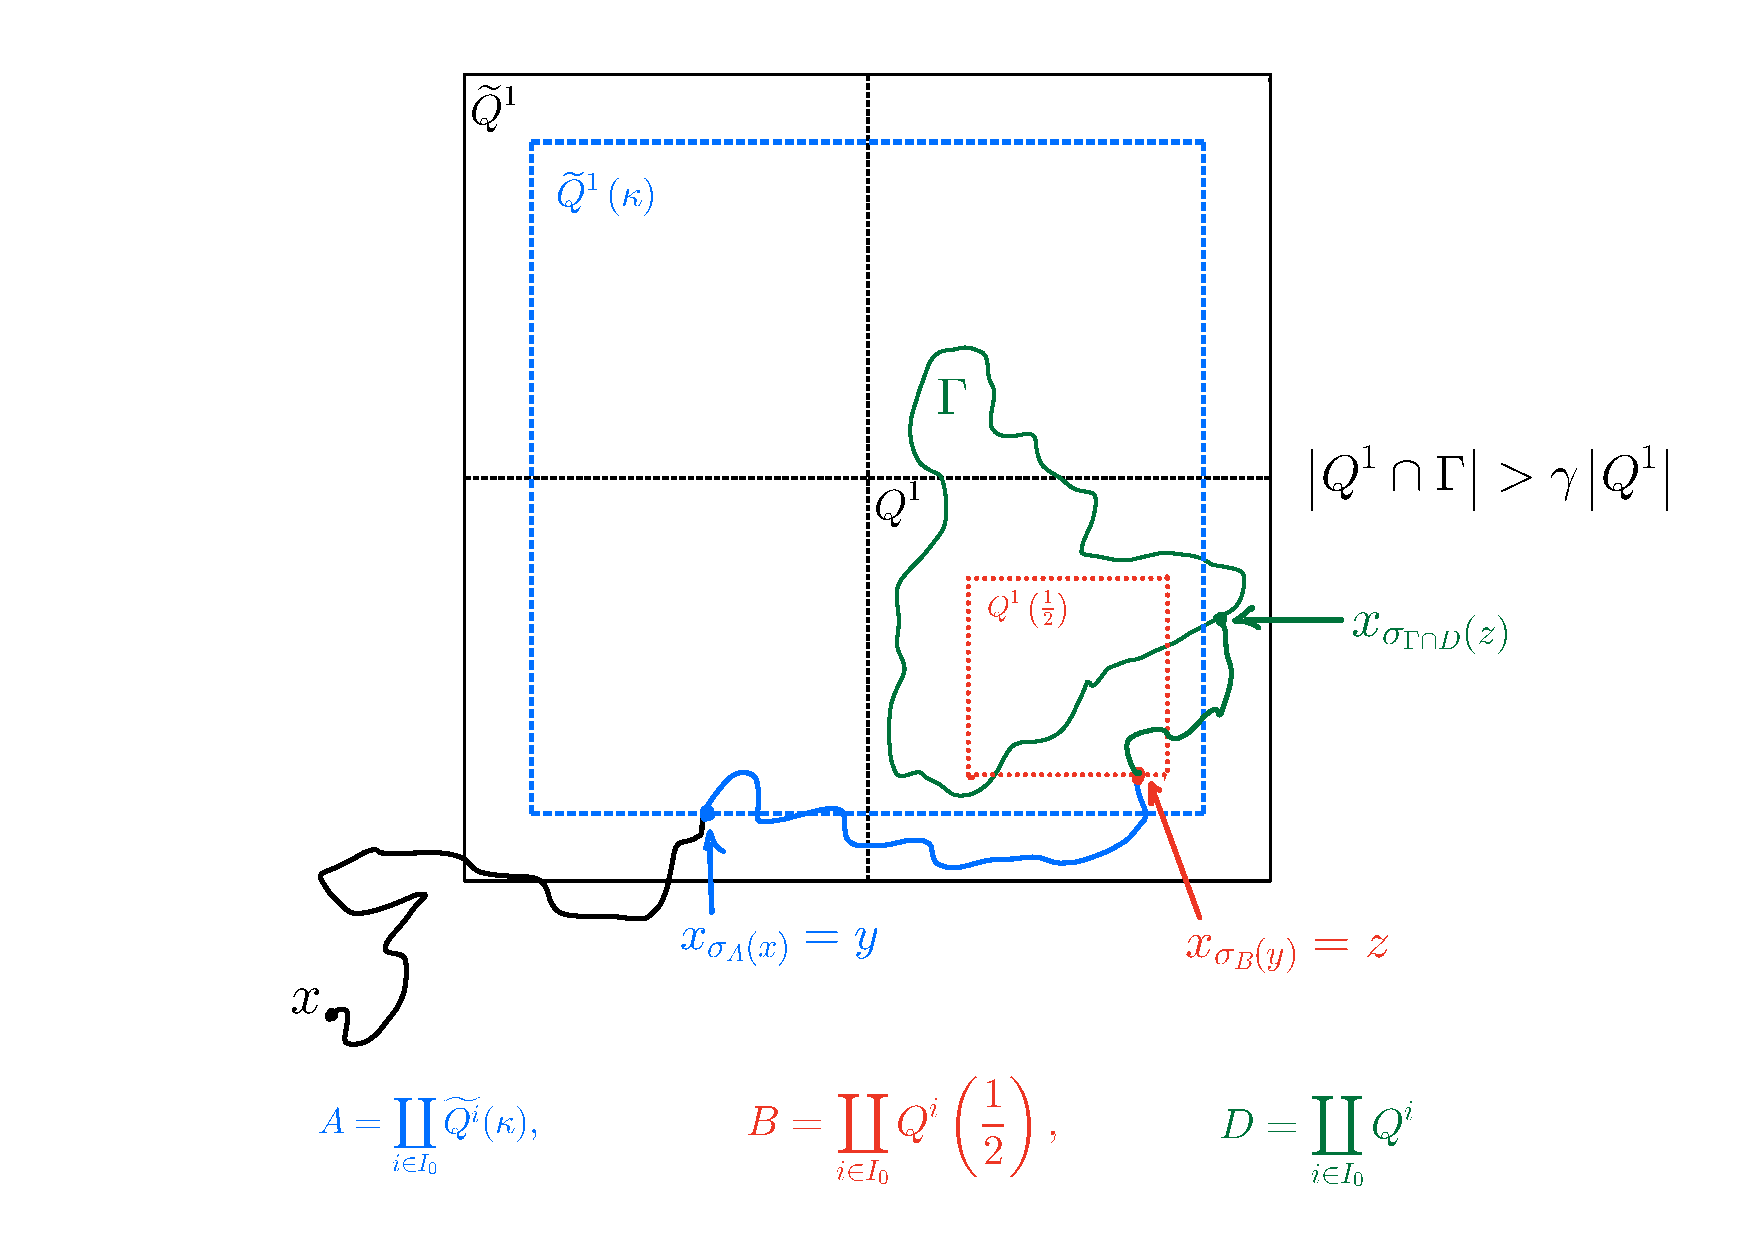
\includegraphics[width=0.9 \textwidth]{hit prob.pdf} 
    \caption{Hitting Prob.} \label{fig:hit} 
    \end{figure}
	
	\section{Harnack Inequality and H\"older estimate}
	In this section, we prove some theorems of Krylov and Safonov \cite{krylov1981certain} concerning (positive) $L$-harmonic functions. Let $\delta\in(0,1)$. Set 
	\begin{align*}
	    \sP(\delta):=\Big\{\{\mP_x\}_{x\in \mR^n}: (\mP_x, X)  \ \textit{is the strong Markov process} \\
        \textit{associate with some } a(\cdot) \in \mS^d_\delta \Big\}.
	\end{align*}
    Let 
    \[
        [u]_{\alpha; D}:=\sup_{x,y\in D} \frac{|u(x)-u(y)|}{|x-y|^\alpha} ~\textit{ and }~ \osc_D u:= \sup_{x\in D} u(x)-\inf_{x\in D} u(x). 
    \]
	
	\begin{theorem}[H\"older estimate]\label{thm:holder}
	  Suppose $u$ is bounded in $Q_1$ and $
	  Lu =0$ in $Q_1$. Then there exist $\alpha$ and $C$ only depending on $d$ and $\delta$ such that
	  \begin{equation}\label{eq:KS-Holder}
	      [u]_{\alpha; Q_{1/2}}\leq C\|u\|_{L^\infty(Q_1)}.
	  \end{equation} \end{theorem}
	\begin{proof}
  \begin{framed}
      {\bf Claim:} there exists a constant $\rho\in (0,1)$ such that  for any $z\in Q_{1/2}$, $r\leq 1/2$, 
		\begin{equation}\label{eq:osc}
		\osc_{Q_{r/2}(z)} \ u\leq \rho \osc_{Q_{r}(z)} \ u. 
		\end{equation}
  \end{framed}
        Assume the claim is true. Suppose that $x,y\in Q_{1/2}$  and $|x-y|\ll1$, let $k\in \mN$ such that $2^{-k-1}\leq |x-y|< 2^{-k}$. 
        \begin{align*}
            |u(x)-u(y)|\leq& \osc_{Q_{2^{-k}}(x)} u \leq \rho \osc_{Q_{2^{-k+1}}(x)} u \leq \cdots \leq C\rho^k\|u\|_{L^\infty(Q_1)}\\
            \leq& C \rho^{-\log_2 |x-y|}\|u\|_{L^\infty(Q_1)}\leq C |x-y|^{-\log_2\rho} \|u\|_{L^\infty(Q_1)}. 
        \end{align*}
        
        Therefore, the above claim implies \eqref{eq:KS-Holder} with $\alpha=\log_2\rho^{-1}$. 
		
  To prove \eqref{eq:osc}. Without loss of generality, we can assume $\inf_{x\in Q_r(z)}u=0$ and $\sup_{x\in Q_r(z)} u=1$. In this case, $\osc_{Q_{r}(z)} \ u=1$. 
		Let $B:=\{x\in Q_{r/2}: u(x)\geq 1/2\}$, we may assume $|B|\geq \frac{1}{2} |Q_{r/2}|$, if not, we replace $u$ by $1-u$. For any $x\in Q_{r/2}$, by  Itô's formula, Theorem \ref{thm:hit} and scaling,  
		\[
            u(x)=\mE_x u(X_{\tau_{Q_r}\wedge \sigma_B})\geq \frac{1}{2}\mP_x (\sigma_B<\tau_{Q_{r}})\geq \frac{1}{2} p(2^{-d-1}). 
        \]
        Hence we get 
		$$
		\osc_{Q_{r/2}(z)} u \leq 1-\frac{1}{2}p(2^{-d-1})=:\rho=\rho \osc_{Q_{r}(z)}u. 
		$$
	\end{proof}
	
	
	
	\begin{theorem}[Harnack inequality]\label{thm:harnack}
 Suppose $a\in \mS^d_\delta$ and $L=a_{ij}\p_{ij}$. There exists $C$ depending only on $\delta$ such that if $u$ is nonnegative, bounded in $Q_4$, and $u(X_{t \wedge \tau_{Q_4}})$ is a martingale, then $u(x) \leq C u(y)$ if $x, y \in Q_1$.
    \end{theorem}
    \begin{proof}
        If we look at $u+\delta$ and let $\delta \rightarrow 0$, we may assume $u>0$. By looking at $C u$, we may assume $\inf _{Q_{1/2}} u=1$. By Theorem , we know that $u$ is Hölder continuous in $Q_1$, so there exists
        \[
            y \in Q_{1 / 2} ~\textit{ such that }~ u(y)=1. 
        \]
        We want to show that $u$ is bounded above by a constant in $Q_1$, where the constant depends only on $\delta$.
        
        By the support theorem and scaling, if $x \in Q_{1/2}$, there exists $\delta$ such that 
        \[
            \mathbb{P}_y\left(\sigma_{Q_{1/2}(x)}<\tau_{Q_2}\right) \geq \delta .
        \]
        By scaling, if $z \in Q_{1/2}(x)$, then $\mathbb{P}_z\left(\sigma_{Q_{1/4}(x)}<\tau_{Q_2}\right) \geq \delta$. So by the strong Markov property,
        \[
            \mathbb{P}_z\left(\sigma_{Q_{1/4}(x)}<\tau_{Q_2}\right) \geq \delta^2 .
        \]
        Repeating and using induction,
        \[
            \mathbb{P}_y\left(\sigma_{Q_{2^{-k}}(x)}<\tau_{Q_2}\right) \geq \delta^k .
        \]
        Then
        \[
            \begin{aligned}
                1 & =u(y) \geq \mathbb{E}_y\left[u\left(X_{\sigma_{Q_{2^{-k}}(x)}}\right) ; \sigma_{Q_{2^{-k}}(x)}<\tau_{Q_2}\right] \\
                & \geq \delta^k\left(\inf _{Q_{2^{-k}}(x)} u\right),
            \end{aligned}
        \]
        or 
        \begin{equation}\label{eq:infu-Qk}
            \inf _{Q_{2^{-k}}(x)} u \leq \delta^{-k} , \quad \forall k\geq 1. 
        \end{equation}
        By the proof of Theorem \ref{thm:holder}, there exists $\rho<1$ such that
        \[
             \osc_{Q_{2^{-k-1}}(x)} u\leq \rho \osc_{Q_{2^{-k}}(x)}u .
        \]
        Take $N$ large so that $\rho^{-N} \geq 1/\left(\delta-\delta^2\right)$.  Then
        \[
            \underset{Q_{2^{N-k}}(x)}{\mathrm{Osc}} u \geq \rho^{-N} \underset{Q_{2^{-k}}(x)}{\operatorname{Osc}} u \geq \frac{1}{\delta-\delta^2} \underset{Q_{2^{-k}}(x)}{\operatorname{Osc}} u .
        \]
        Take $K$ large so that $\sqrt{d} 2^{N-K}<1 / 8$. Suppose there exists $x_0 \in Q_1(y)$ such that $u\left(x_0\right) \geq \delta^{-K-1}$. 
        \begin{framed}
            We will construct a sequence $x_1, x_2, \ldots$ by induction such that $u(x_j)\geq \delta^{-K-j-1}$. 
        \end{framed} Suppose we have $x_j \in Q_{2^{N+1-K-j}}\left(x_{j-1}\right)$ with $u\left(x_j\right) \geq \delta^{-K-j-1}$, $j \leq n$. Since $\left|x_j-x_{j-1}\right|<\sqrt{d} 2^{N+1-K-j}, 1 \leq j \leq n$, and $\left|x_0-y\right| \leq 1$, then $\left|x_n-y\right|<2$. Since $u\left(x_n\right) \geq \delta^{-K-n-1}$ and by  \eqref{eq:infu-Qk}, $\inf _{Q_{2^{-K-n}}(x_n)} u \leq \delta^{-K-n}$, 
        $$
            \underset{Q_{2^{-K-n}}(x_n)}{\operatorname{Osc}} u \geq \delta^{-K-n}\left(\delta^{-1}-1\right) .
        $$
        So $\osc_{Q_{2^{N-K-n}}(x_n)} u \geq \delta^{-K-n-2}$, which implies that there exists $x_{n+1} \in$ $Q_{ 2^{N-K-n}}(x_n)$ with $u\left(x_{n+1}\right) \geq \delta^{-K-n-2}$ because $u$ is nonnegative. By induction we obtain a sequence $x_n$ with $x_n \in Q_3(y)$ and $u\left(x_n\right) \rightarrow \infty$. This contradicts the boundedness of $u$ on $Q_4$. Therefore $u$ is bounded on $Q_1$ by $\delta^{-K-1}$.
    \end{proof}
	

	\chapter{Malliavin's proof of H\"ormander's Theorem}\label{chapt:hormander}
		
	Let $V_0, V_1, \ldots, V_n: \mathbb{R}^d \rightarrow \mathbb{R}^d$ be vector fields satisfying $C^{\infty}$-boundedness conditions. 
	 
     Consider 
     \begin{equation}\label{eq:sde-S}
     	\begin{cases}
     		 \d X_t(x)&= \sum_{=1}^n V_l (X_t)\circ \d W^l_s+ V_0(X_t) \d t= V (X_t)\circ \d W_s+ V_0(X_t) \d t, \\
     		 X_0(x)&=x.
     	\end{cases}
     \end{equation}
     
     The Malliavin calculus is a method originally developed for proving smoothness of $p_t(x,y)$ in the variable $y$, where $p_t(x,y)$ is the transition density of a process associated to an operator with smooth coefficients. The basic idea involves an integration by parts formula in an infinite-dimensional space.

     There are two main approaches, one using the Girsanov transformation and the other using the Ornstein-Uhlenbeck operator. We follow the Girsanov approach pioneered by Bismut \cite{bismut1981martingales} to obtain the integration by parts formula. 

    \section{Integration by parts}
    
    Let $d\geq 1$, and $\xi$ be a $d$-dimensional standard Gaussian random variable. Then 
    \[
    \bP\circ \xi^{-1}(\d x)=\mu(\d x)=\frac{1}{({2\pi})^{\frac{d}{2}}}\e^{-\frac{|x|^2}{2}} \d x. 
    \]
    Suppose $\varphi\in C_c^\infty(\mR^d)$ and $h\in \mR^d$, integration by parts formula yields that 
    \begin{equation}\label{eq:IBP1}
        \begin{aligned}
        \bE \l[\nabla_h \varphi(\xi)\r]=&\frac{1}{(2\pi)^{\frac{d}{2}}}\int_{\mR^d}\nabla_h \varphi(x)\e^{-\frac{|x|^2}{2}} \d x\\
        =&\frac{1}{(2\pi)^{\frac{d}{2}}}\int_{\mR^d} \varphi(x)\<x,h\> \e^{-\frac{|x|^2}{2}} \d x=\bE \l[\varphi(\xi)\<\xi,h\>\r]. 
        \end{aligned}
    \end{equation}
    One can also verify that 
    \begin{equation*}
        \bE [\partial^\alpha \varphi(\xi)]= \bE [\varphi(\xi)P_\alpha(\xi)], 
    \end{equation*}
    where $\alpha\in \mN^d$ and $P_\alpha$ is a polynomial. 
    
    \begin{remark}
    	\begin{enumerate}[(i)]
    		\item Charles Stein also showed that if \eqref{eq:IBP1} holds for all bounded, continuous and piecewise continuously differentiable functions $\varphi$ with $\bE|\varphi'(\xi)|<\infty$, then $\xi$ has a standard normal distribution.
    		\item If $h$ is a smooth vector field on $\mR^d$. Then, 
    		\begin{equation}\label{eq:IBP2}
    			\begin{aligned}
    				\bE \nabla_h \varphi(\xi) =& \int \<\nabla \varphi,h\>  \d \mu=-\int \varphi\,\underbrace{(\div h-\<h,\cdot\>)}_{\div_\mu h} \d \mu\\
    				=&\bE\{ \varphi(\xi) [\<h,\xi\>-\div h(\xi) ]\}. 
    			\end{aligned}
    		\end{equation}
    	\end{enumerate}
    \end{remark}

    The following lemma is a criterion for smooth densities 
    \begin{lemma}
        Suppose $\xi: \Omega \rightarrow \mathbb{R}^d$. Suppose for each $k$ there exists $C_k$ such that
        $$
         \left|\mathbf{E}\nabla^k \varphi(\xi)\right| \leq C_k\|\varphi\|_{\infty}
        $$
        whenever $\varphi \in C^k_c$. Then there exists $\rho$ smooth such that
        $$
        \mathbf{P}(\xi \in A)=\int_A \rho(x) \d x
        $$
        for all Borel sets $A$.
    \end{lemma}
    \begin{proof}
        Let $\mu=\bP\circ \xi^{-1}\in \sP(\mR^d)\subseteq\sD'(\mR^d)$, and $\mu_\eps(x)=\int_{\mR^d}\varrho_\eps(x-y)\mu(\d y)$. By our assumption, for any $\alpha=(\alpha_1,\cdots\alpha_d)\in \mN^d$ with $\alpha_1+\cdots\alpha_d=k$, 
        \[
        \begin{aligned}
            (-1)^{|\alpha|}\<\varphi, \partial^\alpha\mu_\eps\>=&\<\partial^\alpha \varphi, \mu_\eps\>=\<\partial^\alpha \varphi*\varrho_\eps, \mu\>\\
            =&\int_{\mR^d}\partial^\alpha \varphi*\varrho_\eps(x) \mu(\d x)\\
            \leq& C_k\|\varphi\|_\infty, \quad \forall \varphi\in C_c^\infty,~ k\in \mN.
        \end{aligned}
        \]
         This implies that $\sup_{\eps} \|\nabla^k\mu_\eps\|_1\leq C_k$. In the light of Sobolev embedding, one can see that $\sup_{\eps}\|\nabla^k\mu_\eps\|_\infty\leq C'_k$. Therefore, $\mu_\eps\to \rho\in C_b^\infty$. 
    \end{proof}
%    \begin{remark}
%        For a random map $\xi:\Omega\to \mR^d$, if $\xi$ satisfies \eqref{eq:IBP2} and $|\xi|^k$ is integrable for each $k\in \mN$, then $\bP\circ\xi^{-1}$ admits a smooth density.  
%    \end{remark}

    The main tool in the proof is the Malliavin calculus with its integration by part formula in Wiener space (infinite-dimension space), which was developed precisely in order to provide a probabilistic proof of Hörmander's Theorem. It essentially relies on the fact that the image of a Gaussian measure under a ``smooth" submersion that is sufficiently integrable possesses a smooth density with respect to Lebesgue measure. 
    
    Below we set $\Omega=C([0,1];\mR^n)$ and $(\Omega, \cF, \cF_t, \bP)$ be the Wiener space. Then the canonical process $\omega_t$ is a $n$-dimensional Brownian motion under $\bP$. 
    
    \begin{lemma}\label{lem:IBP}
       Suppose $F$ maps $\Omega$ to $\mathbb{R}, F$ is bounded, and $F$ has a bounded Fréchet derivative at each point of $\Omega$. Suppose $h_s$ is adapted and bounded and let $H_t=\int_0^t h_s d s$. Then
       \begin{equation}\label{eq:IBP}
       	    \mathbf{E}\left[D_H F \right]=\mathbf{E}\left[F \int_0^1 h_s \d \omega_s\right]
       \end{equation}
       The left-hand side represents the expectation of the Fréchet derivative at $\omega_{\cdot}$ in the direction $H.(\omega)$.
    \end{lemma}
\begin{proof}
    Let
    $$
      X_t^{\varepsilon}=\omega_t+\varepsilon \int_0^t h_s \d s
    $$

     Let
    $$
         M_t^{\varepsilon}=\exp \left(-\varepsilon \int_0^t h_s \d \omega_s-\frac{\varepsilon^2}{2} \int_0^t\left|h_s\right|^2 \d s\right) .
    $$

     Let $\mathbf{P}_{\varepsilon}$ be defined by $\d \mathbf{P}_{\varepsilon} / \d \mathbf{P}=M_t^{\varepsilon}$ on $\mathcal{F}_t$. By Girsanov's theorem, under $\mathbf{P}_{\varepsilon}$ the process
    $$
        \omega_t-\left\langle \omega,-\varepsilon \int_0 h_s \d \omega_s\right\rangle_t=\omega_t+\varepsilon \int_0^t h_s \d s=X_t^{\varepsilon}
    $$
    is a martingale with the same quadratic variation as $\omega_t$, namely $t$. By Theorem \ref{thm:levy}, under $\mathbf{P}_{\varepsilon}$ the process $X_t$ is a Brownian motion. Therefore
    $$
        \mathbf{E}_{\varepsilon} F\left(X^{\varepsilon}\right)=\mathbf{E} F.
    $$

    On the other hand,
    $$
    \begin{aligned}
    & \mathbf{E}_{\varepsilon} F\left(X^{\varepsilon}\right) \\
    & \quad=\mathbf{E}\left[F\left(\omega+\varepsilon \int_0^\cdot h_s \d s\right) \exp \left(-\varepsilon \int_0^1 h_s \d \omega_s+\frac{\varepsilon^2}{2} \int_0^1\left|h_s\right|^2 \d s\right)\right] .
    \end{aligned}
    $$

    By, the right-hand side of  is independent of $\varepsilon$. We differentiate with respect to $\varepsilon$ and set $\varepsilon=0$. The assumptions on $h$ and $F$ allow us to interchange the operations of differentiation and expectation by use of the dominated convergence theorem and we obtain
    \[
    0=-\mathbf{E}\left[F \int_0^1 h_s \d \omega_s\right]+\mathbf{E} [ D_H F].
    \]
\end{proof}

    \begin{remark}
    	Compare \eqref{eq:IBP2} with \eqref{eq:IBP}. 
    	The adapted process $H$ can be regard as ``divergence-free" vector field on Wiener space. In this case, 
    	\[
    	    \<h,x\> \rightsquigarrow \int_0^1 \dot H_t \d \omega_t``="\int_0^1 \<\dot H, \dot \omega\>\d t~ \mbox{ and }~ ``\div" H=0.
    	\]  
    	
    \end{remark}

    The main examples of $F$ we will consider later is $\varphi(X_t)$, where $\varphi$ is smooth and $X_t$ solves an SDE. However, the It\^o map $F: \omega_{\cdot}\mapsto X_{\cdot}(\omega)$ is even not continuous from $C([0,1];\mR^n)$ to $C([0,1];\mR^d)$. So we need some extension. 

    \medspace
    
    Set 
    \[
        \cH=\l\{H\in C([0,1];\mR^n): H(0)=0, \dot H\in L^2([0,1];\mR^n)\r\}, \quad \<H, H'\>_{\cH}:= \int_0^1 \dot H(s)\cdot \dot H'(s) \d s. 
    \]
    Suppose that $\{H_k\}_{k\in \mN}$ is a normal orthogonal basis of $\cH$. Suppose $F$ maps $\Omega$ to $\mathbb{R}, F$ is bounded, and its Fréchet derivative is also bounded. Set 
    \[
        D_kF:=D_{H_k}F,  \quad D F:= \sum_k D_{H_k}F \, H_k, \quad |DF|_{\cH}= \sqrt{\sum_k ({D_k}F)^2}. 
    \]
    Suppose that $F$, $|DF|_{\cH}$ and $|D^2F|_{HS}$ are bounded. Define 
    \[
        L F = \sum_k \Big(D_kD_kF-\underbrace{D_k F \int_0^1 h_k(s) \d \omega_s}_{``=" \<V, \omega\>_\cH}\Big)
    \]
    Then $L$ is the operator corresponding to the Ornstein-Uhlenbeck operator $\Delta-x\cdot \nabla$ in finite dimensional case, and 
    \begin{exercise}
    	Prove that 
    	\[
    	    \bE [(LF)G]=\bE [F (LG)]. 
    	\]
    \end{exercise}
    Noting that 
    \[
        L(FG)=(LF) G+ F(LG)+2D_kFD_kG, 
    \]
    we have 
    \begin{equation*}
    	\bE [(LF)G]=\bE [F (LG)]=-\bE [D_kFD_kG]. 
    \end{equation*}
    
    Let $p\geq 1$, and $F$ be a function on $\Omega$. We say $F, G$ is in $\sW^{1,p}$ if there exist functionals $F_n$ on $\Omega$ that are bounded, continuous, Fréchet differentiable with bounded and continuous Fréchet derivatives, and with $F_n \rightarrow F$ in $L^p$ and $|D (F_m-F_n)|_{\cH}\rightarrow 0$ in $L^p$. In this case, $F\in L^p$ and for each $k$, and there exists an $\cH$-valued random map, denoted by $DF$ such that  $|DF_n-DF|_\cH \to 0$ in $L^p$.  The general $\sW^{k,p}$-space $(k\geq 1)$ can be defined by the same way. 
    \begin{theorem}\label{thm:IBP}
         Let $p > 1$, $F\in \sW^{1,p}$ and . Assume that $h_t$ is adapted, $H_t=\int_0^t h_s \d s$ and $|H|_{\cH}$ is bounded. Then 
         \begin{enumerate}[(i)]
         	\item   $D_HF_n$ convergets to $\<DF, H\>=:D_H F$ in $L^p$ and 
         	\[
         	    \mathbf{E}[D_H F] =\mathbf{E}\left[F \int_0^1 h_s \d \omega_s\right]. 
         	\]
         	\item it holds that 
         	\[
         	    \varphi(F)\in \sW^{1,p} ~ \mbox{ and }~ D \varphi(F)=\nabla \varphi(F)D F, \quad \forall \varphi\in C^1_b. 
         	\]
         	\item if $F,G\in \sW^{2,p}$  with $p\geq 2$, 
         	\begin{equation}
         		\bE [(LF)G]=\bE [F (LG)]=-\bE [D_kFD_kG]. 
         	\end{equation}
         \end{enumerate}
    \end{theorem}
    \begin{proof}
        We apply Lemma \ref{lem:IBP} discussed above to $F_n$ and let $n \rightarrow \infty$. The convergence of $\mathbf{E}\left[D_H F_n(W)\right]$ can be seen by 
        $$
            |D_HF_n-D_H F_m|=\<H, DF_{n}-DF_{m}\>_{\cH} \leq |H|_{\cH} |D(F_n-F_m)|_{\cH} \to 0 \mbox{ in } L^p, ~ p > 1. 
        $$
        Since 
        \[
            \mathbf{E}\left(\int_0^1 h_s \d \omega_s\right)^{p'}\leq C_p\mathbf{E} \l(\int_0^1\left|h_s\right|^2\d s\r)^{p'/2} \leq C\bE |H|_{\cH}^{p'}<\infty, ~ 1<p'<\infty, 
        \] 
        the convergence of $\mathbf{E}\left[F_n \int_0^1 h_s \d \omega_s\right]$ follows from the $L^p$ convergence of $F_n$ to $F$ in $L^p$ with $p >1$ and the Hölder inequality. The second assertion can be obtained by similar way. 
    \end{proof}
    
    As mentioned above the main examples of $\sW^{k,p}$ functionals will be considered is $\varphi(X_t)$.
    \begin{proposition}
    	Let  $X_t$ be the $d$-dimensional process that is a solution to \eqref{eq:sde-S}. Assume that $\sigma$ and $b$ are $C^{\infty}_b$. Then $X_t \in \sW^{k,p}$ for all $k\geq 1$ and $p>1$.  
    \end{proposition}
    
    \section{Malliavin Matrix}
    Now assume that $F=(F_1,\cdots F_d)$, each $F_i$ is real-valued and $F_i\in \cap_{k,p\geq 1}\sW^{k,p}$, and that $\varphi\in C^\infty_b(\mR^d)$. Let 
    \[
        \gamma_F^{ij}:= \<DF^i, DF^j\>_{\cH}. 
    \]
    Then 
    \[
        D(\varphi(F))= \partial_i \varphi(F) D F^i
    \]
    and 
    \[
        \left\langle D(\varphi(F)), D F^j\right\rangle_\cH= \partial_i \varphi(F) \gamma_F^{i j} . 
    \]
    This yields that 
    \begin{equation}\label{eq:d-phiF}
    	\partial_i \varphi(F)= \left\langle D(\varphi(F)), D F^j\right\rangle_{\cH}\left(\gamma_F^{-1}\right)^{j i},
    \end{equation}
    provided that $\gamma_{F}$ is invertible. 
    
    \begin{exercise}
    	Assume $F\in \cap_{k,p\geq 1}\sW^{k,p}$ and $\gamma_F^{-1}\in \cap_{p\geq 1} L^{p}$. Then 
    	\[
    	    \gamma_F^{-1}\in  \cap_{k,p\geq 1}\sW^{k,p} ~ \mbox{ and }D\gamma_F^{-1}= -\gamma_F^{-1} (D\gamma_F) \gamma_F^{-1}. 
    	\]
    \end{exercise}
    
    \begin{theorem}
    	Suppose that  $F\in \cap_{k,p\geq 1}\sW^{k,p}$ and $\gamma_F^{-1}\in \cap_{p\geq 1} L^{p}$. Then 
    	\[
    	    \l| \bE \nabla \varphi(F) \r| \leq C \|\varphi\|_\infty. 
    	\]
    \end{theorem}
    \begin{proof}
    	Thanks to \eqref{eq:d-phiF} and Theorem \ref{thm:IBP}, 
    	\begin{equation*}
    		\begin{aligned}
    			&\bE \nabla^T \varphi(F)=\bE \l[ \gamma_{F}^{-1} D_k(\varphi(F)) D_k F \r]\\
    			=& \bE \l[D_k( \gamma_{F}^{-1} \varphi(F) D_kF)\r]-\bE \l[ D_k(\gamma_{F}^{-1}) \varphi(F) D_k F\r]- \bE \l[ \gamma_{F}^{-1}\varphi(F) D_kD_k F\r]\\
    			=& \bE \l\{ \varphi(F)  \gamma_{F}^{-1} \l[D_kF \int_0^1 v_k(s) \d \omega_s -D_kD_k F\r] \r\} -\bE \l[ \varphi(F)  D_k(\gamma_{F}^{-1}) D_k F\r] \\
    			=&- \bE \l[ \varphi(F) \gamma_F^{-1} LF\r] + \bE \l[ \varphi(F) \gamma_F^{-1} (D_k\gamma_F) \gamma_F^{-1} (D_k F) \r]. 
    		\end{aligned}
    	\end{equation*}
    	This yields that 
    	\begin{align*}
    		\l| \bE \nabla^T \varphi(F) \r| \leq& \|\varphi\|_\infty  \l\{ \bE [\gamma_F^{-1} LF]+ \bE \l[\gamma_F^{-1} (D_k\gamma_F) \gamma_F^{-1} (D_k F)\r] \r\}\\
    		\leq& C(p, \|F\|_{\sW^{2,p}}, \|\gamma_F^{-1}\|_p) \|\varphi\|_\infty, \quad p\gg 1. 
    	\end{align*}
    \end{proof}
    
    We need to calculate $D_k X_t$, where $X_t$ solves \eqref{eq:sde-S}.  By definition, 
    \[
    X_t(\omega)=x+\int_0^t V \left(X_s\right) \circ \d \omega_s + \int_0^t V_0(X_s) \d s 
    \]
    and 
    \begin{equation*}
    	\begin{aligned}
    		X_t(\omega+\varepsilon H_k)=&x+\int_0^t V \left(X_s(\omega+\varepsilon H_k)\right) \circ \d\left(\omega_s+\varepsilon H_k(s)\right) +\int_0^t V_0(X_s(\omega+\eps H_k)) \d s\\
    		=&x+\int_0^t V\left(X_s(\omega+\varepsilon H_k)\right) \circ \d \omega_s +\varepsilon \int_0^t V\left(X_t(\omega+\varepsilon H_k)\right) h_k(s) \d s \\    		
    		&+\int_0^t V_0(X_s(\omega+\eps H_k)) \d s
    	\end{aligned}
    \end{equation*}
    Taking the difference, dividing by $\eps$, and letting $\eps\to0$, we obtain that
    \begin{equation}\label{eq:DkX}
    	D_k X_t =\int_0^t \partial_j V_l (X_s) D_kX^j_s\circ \d \omega_s^l +\int_0^t \partial_j V_0 (X_s) D_kX^j_s \d s  +   \int_0^t V_l (X_s)h_k^l(s)\d s. 
    \end{equation}
    
    Recall that $J(t)= \nabla X_t$, then 
    \begin{equation}\label{eq:Jacobi2}
        \d J^i_j(t)=\p_l V^i_k \left(X_t\right) J^l_j(t) \circ \d \omega^k_t + \p_l V^i_0(X_t) J^l_j(t)\d t, \quad J(0)=I .
    \end{equation}
   
   Let $Z(t): \Omega \rightarrow \mathbb{R}^{d \times d}$ be the solution to
   \begin{equation}\label{eq:Inv-J}
   	    \d Z^i_j(t)=-Z^i_l(t)  \p_j V^l_k  \left(X_t\right) \circ \d \omega^k_t-Z^i_l (t) V^l_0 \left(X_t\right) \d t, \quad Z(0)=I,
   \end{equation}
    By Itô's formula, one can verify that 
    \begin{equation*}
    	\begin{aligned}
    		\d (Z(t)J(t))= Z(t) \circ \d J(t)+\d Z(t) \circ J(t)=0, 
    	\end{aligned}
    \end{equation*}
    which yields that $Z(t)=J^{-1}(t)$. 
    
    \begin{proposition}
    	\begin{equation}\label{eq:DX-J}
    		D_kX_t=J(t) \int_0^t J^{-1}(s) V(X_s) h_k(s) \d s
    	\end{equation}
    \end{proposition}
    \begin{proof}
    	By It\^o's formula and \eqref{eq:Jacobi2}, 
    	\begin{align*}
    		&\d \l[ J(t) \int_0^t J^{-1}(s) V(X_s) h_k(s) \d s \r]\\
    	=&\d J(t)  \int_0^t J^{-1}(s) V(X_s) h_k(s) \d s + V(X_t) h_k(t) \d t \\
    	\overset{\eqref{eq:Jacobi2}}{=}& \nabla V(X_t) \l[J(t)\int_0^t J^{-1}(s) V(X_s) h_k(s) \d s \r]  \circ \d \omega_t \\
    	&+ \nabla V_0(X_t) \l[J(t)\int_0^t J^{-1}(s) V(X_s) h_k(s) \d s \r]  \d t + V(X_t) h_k(t) \d t 
    	\end{align*}
    	Therefore, $t\mapsto J(t) \int_0^t J^{-1}(s) V(X_s) h_k(s) \d s$ satisfies the same equation as $D_k X_t$, which yields \eqref{eq:DX-J}. 
    \end{proof}
   
    
    

    \section{Hörmander's Theorem}
	
	Let $U(x)=\sum_{i=1}^n U^i(x)\p_i=U^i(x)\partial_i$, $V(x)=V^i(x)\p_i$. Define the Lie Bracket  $[U, V]$ as: 
	\[
	     [U,V](x):= U^i(x) \p_i(V^j(x))\p_j-V^i\p_i(U^j(x))\p_j= [U^i \p_iV^j  -V^i\p_i U^j](x)\p_j
	\]


	Define 
	$$S_0=\{V_i : i>0\}, S_{k+1}=S_k\cup \{[U,V_j]: U\in S_k, j\geq 0\}, $$
	and 
	$$\sV^k=\mbox{span} \{V: V\in S_k\}. $$
	We say that the vector fields $V_0, V_1\cdots, V_n$  satisfy the parabolic H\"ormander condition 
	\begin{align}\label{aspt:H}
	    \bigcup_{k\geq 0} \sV^k(x) = \mR^d, \quad \forall x\in \mR^d   \tag{\bf{H}}
	\end{align} 
	
	Why we consider this kind of condition? 
	
	\begin{theorem}[Stroock-Varadhan's support theorem]
		The law of the solution to \eqref{eq:sde-S} on path space is supported by the closure of those smooth curves that, at every point $(t, x)$, are tangent to the hyperplane spanned by $\{\hat{V}_0(x,t), \cdots , \hat{V}_N(x,t)\}$, where we set 
		$$\hat{V}_0(x,t)=\begin{pmatrix} V_0(x)\\ 1 \end{pmatrix},  \,\,\, \hat{V}_j(x,t)=\begin{pmatrix} V_j(x)\\ 0 \end{pmatrix}, \,\,\, j=1,2\cdots N. $$
	\end{theorem}
	
	
	
	For a smooth manifold $\cM$, recall that $E \subset T\cM$ is a smooth subbundle of dimension $d$ if $E_x \subset T_x\cM$ is a vector space of dimension $d$ at every $x \in \cM$ and if the dependency $x \to E_x$ is smooth. (Locally, $E_x$ is the linear span of finitely many smooth vector fields on $\cM$.) A subbundle is called integrable if, whenever $U, V$ are vector fields on $\cM$ taking values in $E$, their Lie bracket $[U, V ]$ also takes values in $E$.
	With these definitions at hand, recall the well-known Frobenius integrability theorem from differential geometry:
	\begin{theorem}
		Let $\cM $ be a smooth $n-$dimensional manifold and let $E \subset T \cM$ be a smooth vector bundle of dimension $d < n$. Then $E $ is integrable if and only if there (locally) exists a smooth foliation of M into leaves of dimension $d$ such that, for every $x\in  \cM$, the tangent space of the leaf passing through $x$ is given by $E_x$.
		
	\end{theorem}
	
	In view of this result, H\"ormander’s condition is not surprising. Indeed, if we define $E(x,t) = \bigcup_{k\geq 0} \sV^k(x,t)$, then this gives us a subbundle of $\mR^{N+1}$ which
	is integrable. Note that the dimension of $E(x,t)$ could in principle depend on $(t, x)$, but since the dimension is a lower semicontinuous function, it will take its maximal value on an open set. If, on some open set, this maximal value is less than $n + 1$, then support theorem tells us that, there exists a submanifold (with boundary) $\cM^- \subset \cM$ of dimension strictly less than $n$ such that $T_{(y,s)}\cM^- = E_{(y,s)}$ for every $(y, s) \subset \cM^-$ . In particular, all the curves appearing in the Stroock-Varadhan support theorem and supporting the law of the solution to (1.1) must lie in $\cM^-$ until they reach its boundary. As a consequence, since $\cM^-$ is always transverse to the sections with constant $t$, the solutions at time $t$ will, with positive probability, lie in a submanifold of $\cM$ of strictly positive codimension. This immediately implies that the transition probabilities cannot be continuous with respect to Lebesgue measure.
	
	\begin{theorem}
	Consider \eqref{eq:sde-S} and assume that all vector fields have bounded derivatives of all orders. If it satisfies\eqref{aspt:H}, then its solutions admit a smooth density with respect to Lebesgue measure and the corresponding Markov semigroup maps bounded functions into smooth functions.
	\end{theorem}
	
	Let $J_{r,t}$ be the solution of equation: 
	\begin{align}
		J_{r,t}=I+\int_r^t V'_0(X_s) J_{r,s}\d s+\int_r^t V'_j(X_s) J_{r,s}\circ \d W^j_s. 
	\end{align}
	Since $D^i_rX_t$ satisfies: 
	$$D^i_rX_t=V_i(X_r)+\int_r^t V'_0(X_s) D^i_r X_s \d s+\int_r^t V'_j(X_s)D^i_rX_s\circ \d W^j_s. $$
	We get $D^i_rX_t=J_{r,t} V_i(X_t)$. Denote $J_t=J_{0,t}$ for simple, then $J_{s,t}=J_{t}J_{s}^{-1}$ and $J_{t}^{-1}$ satisfies: 
	$$J_t^{-1}=I-\int_0^t J_s^{-1} V'_0(X_s)\d s-\int_0^t J_s^{-1} V'_j(X_s)\circ\d W_s^j. $$
	By the above discussion, 
	$$
	\gamma_t = \sum_{i=1}^N\<D^i X_t, D^i X_t\>=J_t\int_0^t J^{-1}_s V_j(X_s)V^{T}_j(X_s)(J^{-1}_s)^T \d s \,J^T_t=J_t C_t J^T_t. 
	$$
	We only need to prove $\det C_t\in L^{\infty-}$. 
	
	We need the following useful lemma. 
	
	\begin{lemma}\label{Tail}
	Let $M$ be a random, symmetric, positive semidefinite matrix with entries in  $L^{\infty-}.$ Assume that for $p$ sufficient large, there exists a constant $C_p$ and an $\eps_p > 0$ such that
	for $0<\eps<\eps_p$ we have
	$$ \sup_{|\xi|=1}\bP  (\xi^T M \xi\leq \eps)\leq C_p \eps^p. $$
	Then $(\det M)^{-1} \in L^{\infty-}. $
	\end{lemma}
	
	\begin{proof}
		$\forall t>1$, 
		Choose $\{\xi_1,\cdots, \xi_m\}\subset S^N,$ such that $\sup_{|\xi|=1}\min_{k\leq m} |\xi-\xi_k|\leq t^{-2}$ and $m\leq C t^{2N}$. 
		
		$\forall \xi\in S^N$, we can find a vector $\xi_k$ such that,  
		$$\xi^T M\xi = \xi_k^T M\xi_k +\xi_k^TM(\xi-\xi_k)+(\xi-\xi_k)^TM\xi\geq  \xi_k^T M\xi_k-2\|M\|t^{-2}$$
		So we get 
		$$\{\inf_{|\xi|=1} \xi^T M\xi<t^{-1}\}\setminus \bigcup_{k=1}^m \{\xi_k^T M\xi_k<3t^{-1}\}\subset \{ \|M\|>t\}$$
		Now, 
		\begin{equation*}
			\begin{split}
				\bP (\|M^{-1}\|>t)=&\bP  (\inf_{|\xi|=1} \xi^T M\xi<t^{-1})\\
				\leq &\bP \Big( \cup_{k=1}^m \{\xi_k^T M\xi_k<3t^{-1}\}\Big)+\bP (\|M\|>t)\\
				\leq& CC_{2N+p}t^{2N} t^{-2N-p}+\bE  (\|M\|^p)t^{-p}\\
				\leq & C_p t^{-p}
			\end{split}
		\end{equation*}
		$\forall q\geq 1$, 
		\begin{align*}
			\bE  (\det M^{-1})^q\leq& \bE \|M^{-1}\|^q\leq C \int_0^\infty t^{q-1} \bP (\|M^{-1}\|>t)\d t\\\leq& \int_0^\infty 1\wedge t^{q-1}C_{q}  t^{-q-1}\d t<\infty. 
		\end{align*}
	\end{proof}
	
	Fixed $\xi\in S^N$, define $Z_U(t)=\xi^T J_t^{-1}U(X_t)$. 
	Using Ito's formula, 
	\begin{equation}
		\begin{split}
			\d Z_U(t)=&-\xi^T J_t^{-1}V'_0(X_t)U(X_t) \d t- \xi^T J_t^{-1}V'_j(X_t) U(X_t) \circ \d W^j_t\\
			&+\xi^T J_t^{-1}(X_t) U'(X_t)V_0(X_t)\d t+\xi^T J_t^{-1}(X_t) U'(X_t) V_j(X_t)\circ\d W^j_t\\
			=& \xi^T J_t^{-1} [V_0, U](X_t)\d t+\xi^T J_t^{-1} [V_j, U](X_t)\circ\d W^j_t\\
			=& Z_{[V_0, U]}(t)+ Z_{[V_j, U]}(X_t)\circ \d W_t^j\\
			=& \Big[Z_{[V_0, U]}(t)+\frac{1}{2} Z_{[V_j, [V_j, U]]}\Big]\d t+ Z_{[V_j, U]}(X_t) \cdot \d W_t^j.
		\end{split}
	\end{equation}
	
	Before going to prove the main theorem, we need some technical lemmas. 
	\begin{lemma}\label{Inter}
	Suppose $f\in C^{1+\alpha }([0,1])$, then 
	$$\|f\|_{C^1}\leq  C \|f\|_{C^0}^{\frac{\alpha }{1+\alpha }}\cdot \|f\|_{C^{1+\alpha }}^{\frac{1}{1+\alpha }}. $$
	\end{lemma}
	
	\begin{lemma}
	Suppose $Y_t=\int_0^t \sigma_s\d B_s$, $\bE  \|\sigma\|_\infty^p\leq K_p<\infty$, then $\forall \alpha \in(0,\frac{1}{2})$, $p\geq 1$, $\bE  \|Y\|_{C^\alpha }^p\leq C(K,\alpha ,p)$, i.e. $Y\in L^{\infty-}$. 
	\end{lemma}
	\begin{proof}
		Choose $\beta, p$ such that
		$$\alpha +\frac{1}{p}<\beta<\frac{1}{2},$$
		by Sobolev embedding theorem, 
		$$\bE  \|Y\|^p_{C^\alpha }\leq C_{\alpha ,\beta,p}\bE  \|Y\|^p_{W^\beta_p}=C \bE \left(\int_0^1\int_0^1 \frac{|Y_s-Y_t|^p}{|s-t|^{1+\beta p}}\d s\d t\right)= C\int_0^1\int_0^1 \frac{\bE  |Y_s-Y_t|^p}{|s-t|^{1+\beta p}}\d s\d t. $$
		By BDG inequality, 
		$$\bE  |Y_s-Y_t|^p\leq C \bE \Big(\int_s^t \|\sigma_r\|_\infty^2\d r\Big )^{p/2}\leq C_p|s-t|^{p/2}.$$
		Combining the above inequalities,  
		$$\bE  \|Y\|^p_{C^\alpha }\leq C \int_0^1 \int_0^1  |s-t|^{-1-\beta p+p/2}\d s\d t<\infty. $$
	\end{proof}
	
	Suppose $U$ is a smooth vector field with bounded derivatives of all orders. By the above lemma, it's easy to see
	$$\|Z_U\|_{C^\alpha }\in L^{\infty-}. $$
	
	
	\begin{definition}
	Let $\{A\}_{\eps\in(0,1)}$, $\{B\}_{\eps\in(0,1)}$ be two family of random events. 
	
	$A_\eps \rightarrow_\eps B_\eps$ means $\forall p>>1$, there exists a constant $C_p$, such that, 
	$$\bP (A_\eps\setminus B_\eps)\leq C_p\eps^p. $$
	\end{definition}
	
	
	\begin{lemma}[Quantitative version of Doob-Meyer's decomposition]\label{Z-to-ab}
	Let $W$ be a $d-$dimensional Wiener process, $a$ and $b$ be $\mR$ respectively $\mR^d-$ valued adapted processes such that, for $\alpha <1/2$, we have $\|a\|_\alpha , \|b\|_\alpha \in L^{\infty-}$. Moreover, let $Z$ be defined by
	$$Z_t=Z_0+\int_0^t a(s)\d s+\int_0^t b_j(s)\d W^j_s. $$
	Then there exists a constant $r\in(0, 1)$ such that
	$$\{\|Z\|_\infty<\eps\} \rightarrow_\eps \{\|a\|_\infty<\eps^r\} \cap\{\|b\|_{\infty}< \eps^r\} .$$
	\end{lemma}
	\begin{proof}
		\begin{align}\label{Z2} Z_t^2=Z_0^2+\int_0^t (2a_sZ_s+|b(s)|^2)\d s+\int_0^t 2b_j(s) Z_s\d W^j_s. \end{align}
		$\|a\|_\alpha \in L^{\infty-}\rightarrow \{\|a\|_\infty\leq \eps^{-1/4}\}\rightarrow_\eps\varnothing. $ Hence, $\{ \|Z\|_\infty\leq \eps\}\rightarrow_\eps \{\|\int_0^\cdot 2a_sZ_s\d s\|_\infty \leq \eps^{3/4}\}. $ Similarly 
		$\{ \|Z\|_\infty\leq \eps\}\rightarrow_\eps \{\|\int_0^1 |b_j(s)Z_s|^2 \d s\|_\infty \leq \eps^{3/2}\}.$ Using exponential martingale inequality, 
		$$\left\{\Big\|\int_0^1 |b_j(s)Z_s|^2 \d s\Big\|_\infty  \leq \eps^{3/2}\right\}\rightarrow_\eps \left\{ \Big\|\int_0^\cdot  2b_j(s)\d W^j_s\Big\|_\infty \leq \eps^{2/3}\right\}. $$
		From \eqref{Z2}, we get 
		$$\{ \|Z\|_\infty\leq \eps\}\rightarrow_\eps \left\{\int_0^1 |b(s)|^2\d s_\infty\leq \eps^{2/3}\right\}\rightarrow_\eps \left\{\int_0^1 |b(s)|\d s\leq \eps^{1/3}\right\}. $$
		Combining the above relation, \eqref{Inter} and $\{\|b\|_{1/3}\leq \eps^{-1/4}\}\rightarrow_\eps\varnothing$, we get 
		$$\{ \|Z\|_\infty\leq \eps\}\rightarrow_\eps \{\|b\|_\infty\leq \eps^{1/16}\}. $$
		Using the same argument, we can prove 
		$$\{ \|Z\|_\infty\leq \eps\}\rightarrow_\eps \{\|a\|_\infty\leq \eps^{1/80}\}. $$
		
	\end{proof}
	
	\begin{proof}[Proof of Theorem]
		Notice 
		\begin{align}\label{CtoZ}\xi^TC_t\xi=\sum_{j=1}^d \int_0^t |Z_{V_j}(s)|^2\d s.\end{align}
		Using Lemma \ref{Inter}, we get 
		$$\{\xi^TC_t\xi\leq \eps\}\rightarrow_\eps \{ \|Z_{H_k}\|_\infty\leq \eps^q\}$$
		By Lemma \ref{Z-to-ab}, 
		$$\{\xi^TC_t\xi\leq \eps\}\rightarrow_\eps \bigcap_{V\in \sH_k}\{ \|Z_{V}\|_\infty\leq \eps^{q_k}\}$$
		for suitable $q_k > 0.$ Now observe that $Z_V (0) = \<x, U (x_0 )\>$. By H\"ormander’s condition, $\sV^{k'}(x_0) = \mR^N$ for $k$ large enough. However, if $\sV^{k'}(x_0) = \mR^N$, we can pick $V \in \sV^{k'}(x_0)$ such that $|Z_V (0)| =|\<x, V (x_0 )\>| \geq \eps_0$, so that the right-hand-side in the above equation is the empty set. We have thus proved $\{\xi^TC_t\xi \leq\eps\} \rightarrow_\eps \varnothing$. Now, using  Lemma \ref{Tail}, we complete the proof.
	\end{proof}
	 
	%\chapter{Heat Kernel Estimates}\label{chapt:hke}

	\appendix
	\chapter{Useful facts}
	    \setcounter{equation}{0}
	    \renewcommand\theequation{A.\arabic{equation}}
	    \begin{lemma}[Area formula]
	    	Consider a locally Lipschitz function $f: \mR^d \to \mR^d$ and a Borel set $A\subseteq \mR^d$. Then the function $y\mapsto N_A(y):= \mathrm{card}\{f^{-1}(y)\cap A\}\}$ is measurable and 
	    	\begin{equation*}
	    		\int_{A} |\det (\nabla f(x))| \d x = \int_{\mR^n} N_A(y) \d y \geq \sL^d(f(A)). 
	    	\end{equation*}
	    	Consequently, for any $g\geq 0$, 
	    	\begin{equation}\label{eq:area}
	    		\int_{f(A)}g(y)\d y\leq \int_{A} g(f(x)) |\det \nabla f(x)|\d x. 
	    	\end{equation}
	    \end{lemma}
	
	\section{Sobolev spaces}
    Let $W^{k,p}$ denote the Sobolev space consisting of all real-valued functions on $\mR^d$ whose weak derivatives up to order k are functions in $L^p$. Here $k$ is a non-negative integer and $1\leq p<\infty$. The first part of the Sobolev embedding theorem states that 
	\begin{theorem}[Sobolev]\label{thm:Sobolev}
		If $k>l$, and $1\leq p<q<\infty$ are two real numbers such that 
        \[
            \frac{1}{p}-\frac{k-l}{d}=\frac{1}{q}, 
        \]
        then 
        \[
            W^{k,p}\hookrightarrow W^{l,q}. 
        \]
	\end{theorem}
    The second part of the Sobolev embedding theorem applies to embeddings in Hölder spaces $C^{r,\alpha}$. 
    \begin{theorem}[Morrey]\label{thm:Morrey}
        If $d< pk$ and
    \[
        r+\alpha =k-\frac {d}{p}
    \]
    with $\alpha\in (0, 1)$, then one has the embedding 
    \[
        W^{k,p}\hookrightarrow C^{r,\alpha }.
    \]
	
    \end{theorem}
    
	\section{Singular integral}
	Singular integrals are central to harmonic analysis and are intimately connected with the study of partial differential equations. Singular integral is an integral operator
	\[
	    T(f)(x)=\int K(x,y)f(y)\,\d y,
	\]
	whose kernel function $K: \mR^d\times\mR^d\to \mR$ is singular along the diagonal $x=y$. 
	
	Typical examples of integral operators are the Riesz transforms, which are a family of generalizations of the Hilbert transform to Euclidean spaces of dimension $d\geq 2$. Specifically, the Riesz transforms of a complex-valued function $f$ are defined by 
	\[
	    R_{i}f(x)=c_{d}\lim _{\epsilon \to 0}\int _{\mathbf {R}^{d}\backslash B_{\epsilon }(x)}{\frac {(x_{i}-y_{i})f(y)}{|x-y|^{d+1}}}\,\d y, \quad i=1,\cdots d. 
	\]
	The constant $c_d$ is a dimensional normalization given by $c_d={\frac {1}{\pi \omega _{d-1}}}=\frac {\Gamma((d+1)/2)}{\pi ^{(d+1)/2}}$. 
	The limit is written in various ways, often as a principal value, or as a convolution with the tempered distribution
	\[
	    K(x)={\frac {1}{\pi \omega _{d-1}}}\,p.v.{\frac {x_{j}}{|x|^{d+1}}}.
	\]
	
	The Riesz transforms are given by a Fourier multiplier. Indeed, the Fourier transform of $R_i f$ is given by 
	\[
	    \mathcal{F} (R_{i}f)(\xi)=-i \frac{\xi_{i}}{|\xi|} (\mathcal{F} f)(\xi)
	\] 
	A particular consequence of this last observation is that the Riesz transform defines a bounded linear operator in $L^2$.
	
	\begin{theorem}
	For each $i\in \{1,\cdots, d\}$, $R_i$ is bounded on $L^p$ with $p\in (1,\infty)$ and satisfy weak-type (1,1) estimates: 
		\begin{equation}
			\l| \l\{x\in \mR^d:  |R_i f(x)|>\lambda \r\}\r|\leq C_d \|f\|_1/\lambda. 
		\end{equation}\end{theorem}
	
    \section{Interpolation Theorems} 
    
	\begin{lemma}\label{lem:Inter}
	    \begin{enumerate}
	        \item 
         \begin{equation}
             \|\nabla u\|_p\leq C \|\nabla^2 u\|_p^{\frac{1}{2}}\|u\|_p^{\frac{1}{2}}. 
         \end{equation}
            \item \begin{equation}
                [\nabla u]_\alpha\leq C [\nabla^2 u]_\alpha^{\frac{1}{2}} [u]_{\alpha}^{\frac{1}{2}}. 
            \end{equation}
	    \end{enumerate}
	\end{lemma}
	
	
	
	\chapter{Some basic results of  PDEs} 
	
	\section{Monge-Ampère Equation}\label{app:MAE}
     \setcounter{equation}{0}
     \renewcommand\theequation{B.\arabic{equation}}
	To motivate the definition of weak solutions to \eqref{eq:MAE}, given an open set $D \subset \mathbb{R}^n$, consider $u: D \rightarrow \mathbb{R}$ a convex function of class $C^2$ satisfying \eqref{eq:MAE} 
	for some $f: D \rightarrow \mathbb{R}^{+}$. Then given any Borel set $E \subset D$, it follows by the area formula that
	$$
	\int_E f \,\d x=\int_E \operatorname{det} D^2 u\, \d x=|\nabla u(E)| .
	$$
	
	Notice that while the above argument needs $u$ to be of class $C^2$, the identity
	$$
	\int_E f=|\nabla u(E)|
	$$
	makes sense if $u$ is only of class $C^1$. To find a definition when $u$ is merely convex one could try to replace the gradient $\nabla u(x)$ with the subdifferential $\partial u(x)$ and ask for the above equality to hold for any Borel set $E$. Here $\p u(x)$ is given by 
	$$
	\partial u(x):=\left\{p \in \mathbb{R}^d: u(y) \geq u(x)+\langle p, y-x\rangle \quad \forall y \in D\right\}. 
	$$
	This motivates the following definition:
	\begin{definition}
		Given an open set $D \subset \mathbb{R}^n$ and a convex function $u: D \rightarrow \mathbb{R}$, we define the Monge-Ampère measure associated to $u$ by
		$$
		\mu_u(E):=\left|\bigcup_{x \in E} \partial u(x)\right|
		$$
	\end{definition}
	The basic idea of Alexandrov was to say that $u$ is a weak solution
	of \eqref{eq:MAE} if $\mu_u|_{D}=\nu|_{D}$. 
	
	\begin{lemma}
		Let $u,v:D\to \mR$ be convex functions. Then 
		$$
		\mu_{u+v} \geq \mu_u+\mu_v \quad \text { and } \quad \mu_{\lambda u}=\lambda^n \mu_u \quad \forall \lambda>0 .
		$$
	\end{lemma}
	
	\medspace
	
	The following result is  the celebrated Alexandrov maximum principle.
	\begin{theorem}
		Let $D$ be  an open bounded convex set, and let $u: D\to \mR$ be a convex function such that $u|_{\p D}=0$. Then there exists a dimensional constant $C=C(d)$
		such that 
		\begin{equation}\label{eq:abp}
			|u(x)| \leq C(d) \operatorname{diam}(D)^{\frac{d-1}{d}} \operatorname{dist}(x, \partial D)^{\frac{1}{d}}|\partial u(D)|^{\frac{1}{d}},  \quad \forall x \in D. 
		\end{equation}
	\end{theorem}
	\begin{proof}
		Let $(x, u(x))$ be a point on the graph of $u$, and consider the convex ``conical" function $y\mapsto \widehat C_x(y)$ with vertex at $(x, u(x))$ that vanishes on $\p D$. 
		Since $u\leq \widehat C_x$ in $D$ (by the convexity of $u$), Lemma 2.7 implies that 
		$$
		\left|\partial \widehat{C}_x(x)\right| \leq\left|\partial \widehat{C}_x(D)\right| \leq|\partial u(D)| ;
		$$
		so, to conclude the proof, it suffices to bound $|\p \widehat C_x(x)|$ from below. It is not hard to see 
		\begin{itemize}
			\item $\p \widehat{C}_x(x)$ contains the ball $B_\rho$ with $\rho=|u(x)|/\diam (D)$
			\item $\p \widehat{C}_x(x)$ contains a vector of norm $|u(x)|/\dist (x, \p D)$
		\end{itemize}
		Thus, 
		$$
		\partial \widehat{C}_x(x) \supset B_{\varrho}(0) \cup\{q\}, \quad |q|=|u(x)|/\dist (x, \p D). 
		$$
		Since $\p \widehat{C}_x(x)$ is convex, it follows that $\p \widehat{C}_x(x)$ contains the cone $\cC$ generated
		by $q$ and $\Sigma_q:= \{p\in B_\rho: \<p,q\>=0\}$. Therefore 
		$$
		c(d) \rho^{d-1} |q| = |\cC| \leq |\p u(D)|. 
		$$
	\end{proof}
	
	\begin{theorem}
		Let $D$ be an open bounded convex set, and let $\nu$ be a Borel measure on $D$ with $\nu(D)<\infty$. Then there exists a unique convex function $u: D \rightarrow \mathbb{R}$ solving the Dirichlet problem
		$$
		\begin{cases}
			\mu_u=v & \text { in } D \\ u=0 & \text { on } \partial D
		\end{cases}
		$$
	\end{theorem}
	
	\begin{proof}
		By the stability result proved in Lemma below, since any finite measure can be approximated in the weak*
		topology by a finite sum of Dirac deltas, we only need to
		solve the Dirichlet problem  when $\nu=\sum_{i=1}^N \alpha_i \delta_{x_i}$ with $x_i\in D$ and $\alpha_i>0$. To prove existence of a solution, we use the so-called Perron method: we define 
		$$
		\mathcal{S}[\nu]:=\left\{v: \Omega \rightarrow \mathbb{R} \text { convex : }\left.v\right|_{\partial \Omega}=0, \mu_v \geq \nu \text { in } \Omega\right\}
		$$
		and we show that the largest element in $\cS[\nu]$ is the desired solution. We split the argument into several steps.
		
		{\em Step 1}: $\cS[\nu]\neq \emptyset$. To construct an element of $\cS[\nu]$, we consider the ``conical" function $C_{x_i}$, that is $0$ on $\p\Omega$ and takes the value $-1$ at its vertex $x_i$. The Monge–Ampère measure of this function is concentrated at $x_i$ and has mass equal
		to some positive number $\beta_i$ corresponding to the measure of the set of supporting hyperplanes at $x_i$. Now, consider the convex function $\bar v=\sum_{i=1}^N \lambda C_{x_i}$, where $\lambda$ has to be chosen.
		We notice that $\bar v|_{\p \Omega}=0$. In addition, provided $\lambda$ is sufficiently large, Lemma below  
		implies that 
		$$
		\mu_{\bar{v}} \geq \sum_{i=1}^N \mu_{\lambda \hat{C}_{x_i}}=\sum_{i=1}^N \lambda^d \mu_{\hat{C}_{x_i}}=\sum_{i=1}^N \lambda^d \beta_i \delta_{x_i} \geq \sum_{i=1}^N \alpha_i \delta_{x_i} = \nu.
		$$
		This yields $\bar v\in \cS[\nu]$. 
		
		{\em Step 2}: $v_1, v_2 \in \mathcal{S}[\nu] \Rightarrow w:=\max \left\{v_1, v_2\right\} \in \mathcal{S}[\nu]$. Set 
		$$
		\Omega_0:=\left\{v_1=v_2\right\}, \quad \Omega_1:=\left\{v_1>v_2\right\}, \quad \text { and } \quad \Omega_2:=\left\{v_1<v_2\right\}
		$$
		Also, given a Borel set $E\subseteq \Omega$, consider $E_i= E\cap \Omega_i$. 
		
		Since $\Omega_1$ and $\Omega_2$ are open sets, $w|_{\Omega_1}=v_1$ and $w|_{\Omega_2}=v_2$, 
		$$
		\p w(E_1) = \p v_1(E_1), \quad   \p w(E_2) = \p v_2(E_2). 
		$$
		In addition, since $w=v_1$ on $\Omega_0$ and $w\geq v_1$ everywhere else, we have 
		$$
		\p v_1(E) \subseteq \p w(E_0). 
		$$
		Therefore, 
		$$
		\mu_w (E) \geq \mu_{v_1}(E_0\cup E_1)+ \mu_{v_2} (E_2) \geq \nu(E).  
		$$
		
		{\em Step 3}: $u:=\sup _{v \in S[\nu]} v$  belongs to  $S[\nu]$. Let $w_m \uparrow u$ locally uniformly. Then $\mu_{w_m} \rightharpoonup*\mu_u$.  Also, we deduce
		immediately that $u|_{\p\Omega}=0$ by construction;  hence, $u\in \cS[\nu]$. 
		
		{\em Step 4}: The measure $\mu_u$ is supported at the points $\{x_1,\cdots x_N\}$. Otherwise, there exists a set $E\subseteq D$ such that
		$$
		E \cap\left\{x_1, \ldots, x_N\right\}=\emptyset \quad \text { and } \quad|\partial u(E)|=\mu_u(E)>0
		$$
		Therefore, 
		$$
		\l|\partial u(E)\backslash [\cup_{i=1}^{N} \p u(x_i)\cup \p u(\p D)]\r|=|\p u (E)|>0 
		$$
		Let $x_0\in E$ and $p\in \p u(x_0)\backslash [\cup_{i=1}^{N} \p u(x_i)\cup \p u(\p D)]$. Then there exists $\delta>0$ such that
		\begin{equation}\label{eq:baru}
			u \geq \ell_{x_0, p}+2 \delta \quad \text { on }\left\{x_1, \ldots, x_N\right\} \cup \partial \Omega, 
		\end{equation}
		
		where $\ell_{x_0, p}(x)=u(x_0)+p\cdot (x-x_0)$. Set $\bar{u}:=\max\{\ell_{x_0, p}+\delta, u\}\gneqq u$. Notice that $\bar{u}$ is convex, $\bar{u} \geqslant u$, and it follows by \eqref{eq:baru} that $\bar{u}=u$ in a neighborhood of $\left\{x_1, \ldots, x_N\right\} \cup \partial \Omega$. In particular, $\left.\bar{u}\right|_{\partial \Omega}=0$ and $\partial \bar{u}\left(x_i\right)=\partial u\left(x_i\right)$, which implies that $u\log eqq\bar u\in \cS[\nu]$. This is a contradiction. 
		
		{\em Step 5}: $\mu_u=\nu$. By {\em Step 3} and {\em Step 4}, we know that $\mu_{u}=\sum_{i=1}^N \beta_i \delta_{x_i}$ with $\beta_i\geq \alpha_i$. Assume that $\beta_1=\mu_u(x_1)>\nu(x_1)=\alpha_1$. 
	\end{proof}
	
	
	
	\section{Schauder estimate}\label{app:Schauder}
	Let $\sS$ be the Schwartz space of all rapidly decreasing functions, and $\sS'$ the dual space of $\sS$ 
	called Schwartz generalized function (or tempered distribution) space. Given $f\in\sS$,
	let $\sF f=\hat f$  be the Fourier transform defined by
	$$
	\hat f(\xi):=\int_{\mR^d}\e^{-\mathrm{i}2\pi\xi\cdot x} f(x)\d x.
	$$
	Let $\chi:\mR^d\to[0,1]$ be a smooth radial function with 
	$$
	\chi(\xi)=1,\ |\xi|\leq 1,\ \chi(\xi)=0,\ |\xi|\geq 3/2.
	$$
	Define
	$$
	\varphi(\xi):=\chi(\xi)-\chi(2\xi).
	$$
	It is easy to see that $\varphi\geq 0$ and supp $\varphi\subset B_{3/2}\setminus B_{1/2}$ and formally 
	\begin{align}\label{EE1}
		\sum_{j=-k}^k\varphi(2^{-j}\xi)=\chi(2^{-k}\xi)-\chi(2^{k+1}\xi)\stackrel{k\to\infty}{\to} 1.
	\end{align}
	In particular, if $|j-j'|\geq 2$, then
	$$
	\mathrm{supp}\varphi(2^{-j}\cdot)\cap\mathrm{supp}\varphi(2^{-j'}\cdot)=\varnothing.
	$$
	From now on we shall fix such $\chi$ and $\varphi$ and define
	$$
	\Delta_j f:=\sF^{-1}(\varphi(2^{-j}\cdot) \sF f), \quad j\in \mZ.
	$$
	
	We first recall the following useful lemmas. 
	\begin{lemma}
		Let $\alpha\in (0,1)$. For any $u\in C^\alpha$, it holds that 
		\begin{align}\label{Ch}
			\frac{1}{C}\sup_{j\in \mZ} 2^{j\alpha} \|\Delta_j u\|_\infty\leq [u]_{\alpha} \leq C \sup_{j\in \mZ} 2^{j\alpha} \|\Delta_j u\|_\infty, 
		\end{align}
		where 
		\[
		   [u]_\alpha:= \sup_{x\neq y} \frac{|u(x)-u(y)|}{|x-y|^\alpha}, 
		\]
		and $C$ only depends on $d$ and $\alpha$. 
	\end{lemma}
	\begin{proof}
		
	\end{proof}
	
	\begin{lemma}
		There is a constant $C=C(d, \alpha)$, such that for any $u\in C^{2,\alpha}$, 
		\begin{equation}
			[\nabla^2 u]_\alpha \leq C [\Delta u]_\alpha. 
		\end{equation}
	\end{lemma}
	\begin{proof}
		Define 
		$$
		\varphi^{kl} (\xi):= \frac{\xi_k\xi_l}{|\xi|^2} \varphi (\xi),\ \  h^{kl}(x):=\sF^{-1}(\varphi^{kl})(x);  \ \ \varphi^{kl}_j (\xi):= \varphi^{kl}(2^{-j}\xi), \ \ h^{kl}_j(x):=2^{jd} h^{kl}(2^jx). 
		$$
		It is easy to see
		$$
		\p_{kl}u=\sum_{j\in \mZ} u^{kl}_j:=\sum_{j\in \mZ}\varphi^{kl}_j (D) f=\sum_{j\in \mZ} h^{kl}_j* f, 
		$$
		For any $k,l\in \{1,2,\cdots, d\}$, there is a constant $C$ only depending on $\alpha, d$ such that 
		\begin{equation}
			\|u^{kl}_j\|_\infty\leq C 2^{-j\alpha} [f]_\alpha,\quad \forall j\in \mZ. 
		\end{equation}
		For any $x\in \mR^d$, noticing $h^{kl}\in \sS(\mR^d)$ and $\int h^{kl}=\varphi (0)=0$, we get 
		\begin{align*}
			|u^{kl}_j(x)|=&\left|\int_{\mR^d} h^{kl}_j (y)f(x-y) \d y\right|=\left|\int_{\mR^d} h^{kl} (z)(f(x-2^{-j}z)-f(x)) \d z\right| \\
			\leq&  \int_{\mR^d} |h^{kl}(z)| \cdot [f]_\alpha |2^{-j}z|^\alpha  \d z\leq C [f]_\alpha 2^{-j\alpha}. 
		\end{align*}
		By this, 
		\begin{align*}
			|\p_{kl}u(x)-\p_{kl}u(y)|\leq& \sum_{j\leq K} |u^{kl}_j(x)-u^{kl}_j(y)|+\sum_{j>K} |u^{kl}_j(x)-u^{kl}_j(y)|\\
			\leq &  |x-y|\cdot \sum_{j\leq K}   \|\nabla u^{kl}_j\|_\infty+2\sum_{j>K}  \|u^{kl}_j\|_\infty\\
			\leq & C [f]_\alpha |x-y| \sum_{j\leq K} 2^{(1-\alpha)j}+ C [f]_\alpha\sum_{j>K} 2^{-j\alpha}\\
			\leq & C [f]_\alpha \left(|x-y| 2^{(1-\alpha)K} + 2^{-\alpha K}\right)
		\end{align*}
		Choosing $K\in \mZ$ such that $2^{-K}\leq |x-y|<2^{-K+1}$, we obtain 
		$$
		|\p_{kl}u(x)-\p_{kl}u(y)|\leq C_1[f]_\alpha\cdot |x-y|^\alpha.  
		$$
		So we complete our proof. 
	\end{proof}
	
	\begin{lemma}\label{Le-Ele}
		Suppose $f: \mR_+ \to\mR_+$, and for any $0\leq s<t\leq 1$, 
		$$
		f(s)\leq \theta f(t)+ A(t-s)^{-\gamma} +B, 
		$$ 
		for some $\gamma>0$, then 
		\begin{equation}
			f(s)\leq C(\gamma, \theta) \left( A (t-s)^{-\gamma} +B\right)
		\end{equation}
	\end{lemma}
	\begin{proof}
		Let $t_0=t$, $t_i=s+(1-\tau)\tau^i (t-s)$, where $\tau\in (\theta^{1/\gamma},1)$. By iteration, 
		\begin{align*}
			f(s)=& f(t_{0})\leq \theta f(t_{1})+ A(t_{i}-t_{i+1})^{-\gamma}+B\\
			\leq & \theta^2 f(t_{2})+\theta A(t_{2}-t_1)^{-\gamma}+\theta B+A(t_{1}-t_{0})^{-\gamma}+B\\
			\leq&  \cdots \leq \theta^k f(t_k)+ A (1-\tau)^{-\gamma} (t-s)^{-\gamma} \sum_{i=0}^{k-1} (\theta \tau^{-\gamma})^i +B\sum_{i=0}^{k-1} \theta^i\\
			\leq &C\left(\frac{A}{(t-s)^\gamma}+B\right). 
		\end{align*}
		
	\end{proof}
	\begin{theorem}
		Suppose 
		\begin{equation}\label{Eq-2}
			Lu =a^{ij}\p_{ij} u+b^i \p_i u+cu=f, \quad \textit{in}\ B_R, 
		\end{equation}
		and 
		\begin{equation}
			\delta |\xi|^2\leq a^{ij}\xi_i\xi_j, 
		\end{equation}
		\begin{equation}
            \begin{aligned}
                (\|a\|_{L^\infty(B_R)}+ R^\alpha [a]_{\alpha; B_R})&+(R\|b\|_{L^\infty(B_R)}+ R^{1+\alpha} [b]_{\alpha; B_R})\\
                &+(R^2\|c\|_{L^\infty(B_R)}+ R^{2+\alpha} [c]_{\alpha; B_R}) \leq \Lambda.
            \end{aligned} 
		\end{equation}
		Then, 
		$$
		[\nabla^2 u]_{\alpha; B_{R/2}}\leq C \Big\{ [f]_{\alpha;B_R} +R^{-\alpha}\|f\|_{L^\infty(B_R)}+R^{-2-\alpha} \|u\|_{L^\infty(B_R)} \Big\}. 
		$$
	\end{theorem}
	\begin{proof}
		Suppose $\eta\in C_c^\infty$, $\eta(x)=1$ if $x\in B_{\rho}$, $\eta(x)=0$ if $x\in B^c_{r}$ and 
		$$(r-\rho)^{k}\|\nabla^k \eta \|_\infty+(r-\rho)^{k+\alpha}[\nabla^k \eta]_{\alpha}  \leq C(d, k). $$ 
		Let $v:=u\eta$, then 
		$$
		a^{ij}_o \p_{ij} v= (a^{ij}_o-a^{ij})\eta\cdot \p_{ij} u+2a^{ij}_o \p_i u\p_j \eta+ a^{ij}_o u\p_{ij}\eta+(b^i \p_i u )\cdot\eta+ (cu)\cdot \eta+ f\eta. 
		$$
		\begin{align*}
			[\nabla^2 u]_{\alpha; B_{\rho}}\leq& [\nabla^2 v]_\alpha\leq  C_1\Big\{  r^\alpha[\nabla^2 u]_{\alpha; B_{r}}+(r-\rho)^{-\alpha} \|\nabla^2 u\|_{L^\infty(B_{r})}\\
			&+ (r-\rho)^{-1} [\nabla u]_{\alpha; B_{r}}+(r-\rho)^{-1-\alpha} \|\nabla u\|_{L^\infty(B_{r})}+ (r-\rho)^{-2} [u]_{\alpha; B_{r}}\\
			&+(r-\rho)^{-2-\alpha} \|u\|_{L^\infty(B_{r})}+[f]_{\alpha; B_{r}}+(r-\rho)^{-\alpha}\|f\|_{L^\infty(B_{r})}\Big\}
		\end{align*}
		There is a constant $r_0\in (0,1)$ such that $C_1 r_0^\alpha\leq 1/4$. By interpolation, there is a constant $C$ such that 
		\begin{align*}
			&C_1\Big\{ (r-\rho)^{-\alpha} \|\nabla^2 u\|_{L^\infty(B_{r})}+ (r-\rho)^{-1} [\nabla u]_{\alpha; B_{r}}+(r-\rho)^{-1-\alpha} \|\nabla u\|_{L^\infty(B_{r})}+ (r-\rho)^{-2} [u]_{\alpha; B_{r}}\\
			&+(r-\rho)^{-2-\alpha} \|u\|_{L^\infty(B_{r})}\Big\}
			\leq \frac{1}{4} [\nabla^2 u]_{\alpha; B_{r}} +C (r-\rho)^{-2-\alpha} \|u\|_{L^\infty(B_r)}
		\end{align*}
		Combing the above inequalities and \ref{Le-Ele}, we obtain that for any $0\leq \rho<r\leq r_0$, 
		$$
		[\nabla^2 u]_{\alpha; B_\rho}\leq C \Big\{(r-\rho)^{-2-\alpha} \|u\|_{L^\infty(B_r)}+ [f]_{\alpha; B_{r}}+(r-\rho)^{-\alpha}\|f\|_{L^\infty(B_{r})}\Big\}.
		$$
		Hence, by choosing $\rho=\tfrac{r_0}{2}$, $r=r_0$ and using finite cover technique, we find if $u$ satisfies $Lu=f$ in $B_1$ and 
		$$\lambda |\xi|^2\leq a^{ij}\xi_i\xi_j; \quad \|a\|_{C^\alpha(B_1)}+\|b\|_{C^\alpha(B_1)}+\|c\|_{C^\alpha(B_1)}\leq \Lambda, $$
		then 
		$$
		[\nabla^2 u]_{\alpha; B_{1/2}}\leq C \Big\{ [f]_{\alpha;B_1} + \|f\|_{L^\infty(B_1)}+ \|u\|_{L^\infty(B_1)} \Big\}. 
		$$
		By rescaling, it is easy to obtain our result. 
	\end{proof}
	
	
	
	
	
    
	

	\bibliographystyle{alpha} 
	\bibliography{mybib}
 
	\printindex
	
\end{document}